%!TEX root = Thesis.tex

\chapter{Introduction}
\label{chapter:introduction}

This thesis provides an account of research into a group of diphosphine ligands with a rigid xanthene backbone and \tBu{} substituents on the phosphorus atoms.  The three ligands have different groups in the bridgehead position of the backbone (\ce{CMe2}, \ce{SiMe2}, or S) which changes the natural bite-angle of the ligand.  The coordination chemistry of these \tBuxantphos{} ligands with late-transition metals has been investigated with a focus on metal complexes that may form in catalytic reactions.

%\fixme{Stephen wants to fix this with me, re-write with research objectives in mind.}



\section{Tertiary Phosphine Ligands}

Transition metal complexes have a number of different applications, from use as homogeneous catalysts, to chemotherapeutics, or organic light emitting diodes.\cite{Lamansky2001, Rosenberg1969, Wilson2013}  Tertiary phosphine ligands are some of the most ubiquitous in coordination chemistry.  Phosphines coordinate to transition metals by donation of the lone pair on the phosphorus atom forming a $\sigma$-bond and $\pi$-back-donation into the P-C anti-bonding $\sigma^*$ orbitals which have $\pi$ symmetry.\cite{Orpen1990}  This combination forms stable coordination complexes with a range of different transition metals and oxidation states.  A large array of different phosphine ligands are known with a range of different steric and electronic properties.  These allow the phosphines to impart different physical environments and electron densities on the metal centre, which can result in different reactivities of the complexes.  Due to this, phosphine ligands are frequently used as ancillary ligands in a wide range of different catalytic systems including industrial-scale processes.\cite{Noyori2002, Nicolaou2005, Knowles2002}


%The strong coordination of phosphine ligands means they are not readily displaced in a catalytic process, resulting in increased lifetimes of the catalytic species and consequently higher \glspl{TON}.  The array of different phosphine ligands available allows control over the steric and electronic properties that are imparted to the metal centre resulting in  improved selectivity or activity in different catalytic systems.  As such, phosphine ligands have been used as ancillary ligands in a wide range of different catalytic processes including industrial-scale processes.
\subsection{Electronic and Steric Properties}

As the chemical properties of the metal in a coordination complex are controlled largely by the coordinated ligands, several studies have quantified the electronic and steric properties of phosphine ligands.\cite{Tolman1977, Banger2009, Dunne1991, Roodt2003, Mann1980, Tiburcio2006, Tolman1970}  

Investigations of electronic properties of ligands involve the measurement of the \ce{C#O} stretching frequency in a metal carbonyl complex such as [Ni\ce{(CO)3L}], [Mo\ce{(CO)5L}] or [Rh(CO)Cl\ce{L2}].\footnote{The nomenclature used in this thesis is in accordance with the Nomenclature of Inorganic Chemistry - IUPAC Recommendations 2005.\cite{IUPAC2005}}\cite{Tolman1977, Tolman1970, Roodt2003, Banger2009}  If metal with a spin active isotope such as rhodium or platinum is used, then the value of the one-bond metal-phosphorus coupling constant can also offer insight into the electronic properties of the phosphine ligand.\cite{Mann1980, Pregosin2012, Roodt2003, Banger2009}  The value of the one-bond phosphorus-selenium coupling constant in a phosphinoselenide has been used as a way to study the electronic properties of phosphines.\cite{Beckmann2011, Allman1982}  The phosphinoselenides are readily synthesised, air-stable solids which avoid the need for transition metals or the use of toxic gases.  A comparison of the different techniques used to measure the electronic properties has shown good correlation between the various series.\cite{Banger2009}

%The electronic properties can be investigated in a number of different ways.  However, the most typical way involves the synthesis of a metal complex which has an easily measured parameter.  The first investigation into these properties was performed by synthesising a series of nickel(0) carbonyl complexes of the type \ce{[Ni(CO)3L]}\footnote{The nomenclature used in this thesis is based on the Nomenclature of Inorganic Chemistry - IUPAC Recommendations 2005.\cite{IUPAC2005}}   and determining the carbonyl stretching frequency.\cite{Tolman1977}  The carbonyl stretching frequency is highly dependent on the electronic properties of the metal centre which is controlled by the ancillary ligands.  Carbonyl ligands are strong $\pi$-acceptor ligands and coordinate to the metal \emph{via} donation from a $\sigma$ orbital and back donation into the $\pi^*$ anti-bonding orbital of the \ce{C#O} bond.  As this is an anti-bonding orbital, additional electron density decreased the C-O bond order and thus the observed stretching frequency is reduced.  As such, phosphines with strongly electron donating substituents such as alkyl groups result in a large reduction in the stretching frequency while phosphines with electron withdrawing substituents such as aryl groups have a smaller shift.   In some unusual cases with very strongly electron withdrawing substituents on the phosphorus centre the \ce{C#O} stretch can be shifted to higher wave numbers than that reported for free, uncoordinated carbon monoxide (2143 \si{\per\cm}).\cite{Anderson2014}

%A number of other related approaches have been utilised in the literature to analyse the electronic properties of tertiary phosphines.  The C-O stretching frequency in the octahedral \ce{[Mo(CO)5L]} complex and square planar \ce{Rh(CO)ClL2]} complex have been used to further investigate the electronic influence of phosphines on the metal centre.\cite{Banger2009}  The series correlate well though the specific values vary as the metals also have different electronic character.   Typically the values for the Tolman nickel series are from 2056.1-2110.8 \si{\per\cm} (\ce{PtBu3, PF3}) for the nickel series, 2066-2104 \si{\per\cm} (\ce{P(o-Tol)3}, \ce{P(CF3)3}) for the molybdenum series and 1943-2016 \si{\per\cm} (\ce{PCy3}, \ce{P(OPh)3}) for the rhodium complexes.  In general alkyl substituents like Me, Et, \fixme{iPr}, \tBu{} and cyclohexyl donate more electron density than phenyl substituents and phosphite ligands (bonding to phosphorus through an oxygen).  Fluorophosphines and fluoroalkylsubstituted phosphines are most commonly the least electron donating as the strong electron negativity of the fluorine atoms withdraws electron density from the phosphorus, making the lone pair less available for coordination to the metal.  

%One point of interest with the rhodium complexes is that as there are two phosphorus atoms coordinated to the rhodium this gives the possibility of \cis{} or \trans{} isomers.  The most commonly reported isomer \fixme{check this} is the \trans{} isomer, although the technique has also been used to study \cis{} complexes of diphosphine ligands.  This indicates the sensitivity of using carbonyl ligands as a probe for the electronic properties as, generally the strongest effect is felt for ligands in a \trans{} position (c.f \trans{} influence and \trans{} effect).
%
%The values for the rhodium complexes are typically shifted further to lower wave numbers than the values for the nickel and the molybdenum series.  This is expected as rhodium is a late transition-metal and thus more electron rich than the mid-series molybdenum and the first-row nickel.  The Tolman series of \ce{[Ni(CO)3L]} complexes is the most well-known and henceforth has the largest number of reported values in the literature, both the molybdenum and rhodium series have been shown to correlate well with the nickel series.  

%\Gls{NMR} spectroscopy has also been used to investigate the electronic properties of phosphine ligands.  \phosphorus{} \gls{NMR} is a very sensitive technique, and can be used to probe complexes which may be too unstable to obtain an infrared spectrum.   A further advantage is that the probe for the electronic properties in this case is a phosphorus-atom coupling constant.  Thus the phosphorus is directly incorporated into the probe meaning that it can give a better understanding of the phosphorus directly rather than an overview of many potential synergistic effects.  The previously mentioned \ce{[Rh(CO)Cl(L)2]} complexes and \trans-\ce{[PtCl2L2]} have been used to investigate the electronic properties of various phosphine ligands.  Rhodium-103 and platinum-195 both have spins of 1/2 meaning that they couple to the coordinated phosphorus atoms.  While \ce{^{103}Rh} is 100\% abundant, \Pt{} is only 34\% abundant with the other isotopes not spin active.  Hence the \phosphorus{} \gls{NMR} spectrum in \ce{[Rh(CO)Cl(L)2]} appears as a doublet while in \trans-\ce{[PtCl2L2]} a singlet with \Pt{} satellites is observed.  The coupling constants for \ce{[Rh(CO)Cl(L)2]} range from 114.7 - 193.9 Hz for \ce{PMe3} to \ce{POMe3} with most values falling between 114.7 and 142.3 Hz.  For \trans-\ce{[PtCl2L2]} the values range from 2379 Hz for the electron rich \ce{PMe3} and 5694 Hz for the electron poor, \ce{P(OEt)3} with most  of the values between 2379 and 3145 Hz.  The values vary greatly between the metals as platinum has a greater gyromagnetic ratio than rhodium.\cite{Pregosin2012}  However, the trends are consistent between the series.  Coupling constants are influenced by the amount of s-character that a given bond has.  Generally the more s-character the higher the coupling constant for that bond.  According to Bent's rule ``atomic s-character concentrates in orbitals directed towards electropositive substituents''.  Thus the greater the metal-phosphorus coupling constant the more s-character is present in the M-P bond, thus indicating a greater degree of electronegative substituents, and thus the less electron donating the phosphine ligand will be.  In this case we see that the lower coupling constants are found for the trialkyl phosphines while the higher coupling constants are found for the tri(fluoroalkyl)phosphines and phosphinites.  

%Although phosphines are typically studied for their use as ligands in transition metal complexes, it is possible to investigate their electronic properties without using metals.  Phosphines react readily with chalcogens resulting in oxidation of the phosphorus to a P(V) species.  These molecules are generally easily synthesised and air-stable solids.  Selenium has a number of different isotopes with mass numbers 76, 77, 78, 80 and 82.  All of these have a nuclear spin of zero except \ce{^{77}Se} with a spin of -1/2.  \ce{^{77}Se} is only 7.6\% abundant, thus the \phosphorus{} \gls{NMR} signal appears as a singlet with selenium satellite.  The phosphine selenides show coupling constants of 673 - 805 Hz, though some higher values have been observed.  Again these rely on the changing s-character resulting from the different electronegativities of the phosphorus atom's substituents.  The more electronegative the substituents are, the more s-character will be in the phosphorus selenium bond, thus resulting in a higher coupling constant.  The trend is the same as previous examples whereby the trialkyl phosphines have the lowest coupling constants indicating an electron rich phosphorus.  The phenyl substituted phosphines have higher coupling constants indicating their less electron rich nature.  The fluoro substituted phosphines, phosphinites and phosphites have much higher coupling constants indicating their electron withdrawing character.  

The steric properties of different ligands have also been examined from a quantitative perspective.  The Tolman cone angle is the angle formed at the apex of a cone centred at 2.28 \si{\angstrom} from the phosphorus atom where the outer edges of the cone lie at the Van der Waals radii of the outer most atom of the ligand.  The Tolman cone angle has some limitations: it was originally determined using physical molecular models with idealised bond lengths and van der Waals radii while actual molecules may vary from these values.  In addition, the Tolman cone angle is a maximum cone angle which works well for approximately symmetrical spherical substituents such as \ce{PMe3} or \ce{P^{t}Bu3}, however when planar rings, such as phenyl substituents, are present these can rotate readily, resulting in much larger changes to the cone angle than a trialkyl phosphine would exhibit.  The Tolman cone angles for aryl systems tends to be larger than the crystallographically determined cone angle.

%As expected we see that the largest cone angles are for the \ce{P(mesityl)3,} \ce{P(o-Tol)3}, \ce{P(C6F5)3}, \ce{PtBu3} and \ce{P(neopentyl)3} with values of 212, 194, 184, 182 and 180\degrees.  These ligands all have a significant steric impact on the phosphorus and thus will reduce the available space around a transition metal in a coordination complex.   The smallest cone angles are for \ce{P(NCH2CH2)3}, \ce{P(OEt)3} and \ce{P(OCH2CH2Cl)3} with values of 108, 109 and 110\degrees{} respectively.  The smallest phosphine with non-heteroatom substituents is \ce{PMe3} with a cone angle of 118\degrees.  The other common trialkyl phosphines (\ce{P(Et)3}, \ce{P(Bu)3} and \ce{P(Pr)3}) all have a cone angle of 132\degrees indicating that beyond an ethyl group further increases in change length has little impact.  Branching of the chain does have an impact however, with \ce{P(i-Bu)3}, \ce{P(iPr)3}, \ce{P(sec-Bu)3} and \ce{P(tBu)3} having cone angles of 143, 160, 160 and 182 respectively indicating that branching has a significant impact.  

%===========================================================================
\subsection{Diphosphine Ligands}

Diphosphine ligands consist of two tertiary phosphines linked by a backbone.  A selection of diphosphine ligands are shown in Figure \ref{diphosphineligands}.  Most commonly, the backbone is a carbon skeleton such as an ethane, propane, or xylene group as found in \acrshort{dppe}, \acrshort{dppp}, or \acrshort{dbpx}.  Larger groups can also be used as backbones, such as the binapthyl ligand \acrshort{BINAP}, or the \acrshort{BISBI} system.  The backbones can also include heteroatoms such as \acrshort{diop} or \acrshort{DPEphos}, or transition metal as in the ferrocene molecule found in \acrshort{dppf}.  The backbone can also be used to produce chiral ligands including \acrshort{BINAP}, \acrshort{diop} or \acrshort{SEGphos}, which can be used for asymmetric catalysis.\cite{Noyori2002, Agbossou1995, Shimizu2007}  Diphosphine ligands typically chelate to transition metals, resulting in enhanced stability through the chelate effect.  The chelate effect is an entropic effect, where a complex with a bidentate ligand is observed to have increased thermodynamic stability compared to the same complex with similar monodentate ligands.\cite{Housecroft2005}  In monophosphine complexes, the monophosphine must compete with the other components in the reaction mixture as there is no entropic driver for a second molecule of the monophosphine to coordinate over any other ligands in the system.  Hence the increased thermodynamic stability of complexes with bidentate chelating ligands compared to the same complex with analogous monodentate ligands.  

\begin{figure}[htbp]
\centering
\begin{subfigure}[b]{0.3\textwidth}
	\centering
	
\includegraphics{../Figures/Diphosphines/dppe.eps}
	\caption{dppe}
	\label{dppe}
\end{subfigure}
~
\begin{subfigure}[b]{0.3\textwidth}
	\centering
	
\includegraphics{../Figures/Diphosphines/dppp.eps}
	\caption{dppp}
	\label{dppp}
\end{subfigure}
~
\begin{subfigure}[b]{0.3\textwidth}
	\centering
	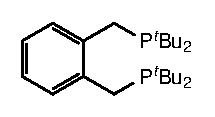
\includegraphics{../Figures/Diphosphines/dbpx.eps}
	\caption{dbpx}
	\label{dbpx}
\end{subfigure}
\\
\vspace{0.5cm}
\begin{subfigure}[b]{0.3\textwidth}
	\centering
	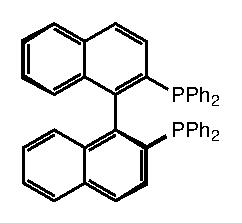
\includegraphics{../Figures/Diphosphines/BINAP.eps}
	\caption{BINAP}
	\label{BINAP}
\end{subfigure}
~
\begin{subfigure}[b]{0.3\textwidth}
	\centering
	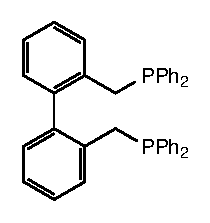
\includegraphics{../Figures/Diphosphines/BISBI.eps}
	\caption{BISBI}
	\label{BISBI}
\end{subfigure}
~
\begin{subfigure}[b]{0.3\textwidth}
	\centering
	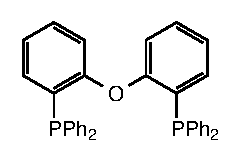
\includegraphics{../Figures/Xantphosderivatives/DPEphos.eps}
	\caption{DPEphos}
	\label{DPEphos}
\end{subfigure}
\\
\vspace{0.5cm}
\begin{subfigure}[b]{0.3\textwidth}
	\centering
	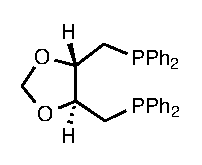
\includegraphics{../Figures/Diphosphines/DIOP.eps}
	\caption{diop}
	\label{diop}
\end{subfigure}
~
\begin{subfigure}[b]{0.3\textwidth}
	\centering
	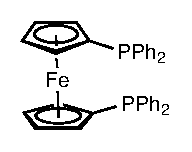
\includegraphics{../Figures/Diphosphines/dppf.eps}
	\caption{dppf}
	\label{dppf}
\end{subfigure}
~
\begin{subfigure}[b]{0.3\textwidth}
	\centering
	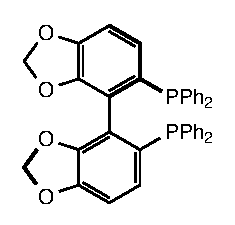
\includegraphics{../Figures/Diphosphines/SEGphos.eps}
	\caption{SEGphos}
	\label{SEGphos}
\end{subfigure}
\\
\caption[Selection of diphosphine ligands]{Selection of diphosphine ligands.}
\label{diphosphineligands}
\end{figure}

The electronic and steric properties of diphosphines ligands can be described using the techniques developed for monophosphines.\cite{Tolman1977, Banger2009, Dunne1991, Roodt2003, Mann1980, Tiburcio2006, Tolman1970}  The bite-angle, defined as the P-M-P angle in a transition-metal complex (Figure \ref{Biteangle}), can also be used to quantify and compare different diphosphine ligands.  The natural bite-angle is defined as the P-Rh-P angle calculated by molecular modelling using a rhodium atom with fixed Rh-P distances of 2.315 \si{\angstrom}.\cite{Casey1990}  The bite-angle for a given complex can also be measured from an X-ray crystal structure.  The original development of the natural bite-angle parameter included a comparison of the natural and crystallographic bite-angles for seven different complexes, showing good correlation between the natural and crystallographic bite-angles.\cite{Casey1990}  A further study in 1999 showed that, for a range of different diphosphine ligands, the crystallographic bite-angles occur within a very narrow range which correlate well with the natural bite-angles.\cite{Dierkes1999}

\begin{figure}[ht]
\centering
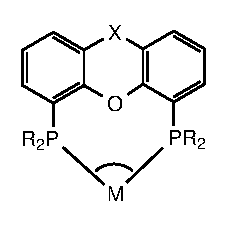
\includegraphics[]{../Figures/Biteangle.eps}
\caption[The bite angle]{The bite angle}
\label{Biteangle}
\end{figure}

When used as ancillary ligands in transition metal catalysts, diphosphines can result in different product distributions compared with the analogous monophosphines.  The catalytic reaction of ethene and carbon monoxide, in a methanol solution, produced short chain oligomers when [Pd(MeCN\ce{)4](BF4)2} was used as the precatalyst with an excess of a monophosphine ligand such as triphenylphosphine.\cite{Lai1984}  Changing to a stoichiometric amount of a chelating diphosphine with  [Pd(OAc\ce{)2]}, resulted in the co-polymerisation of carbon monoxide and ethene giving polyketone, indicating that the rate of chain termination is faster for mono\-phosphine complexes than in the diphosphine complexes.\cite{Drent1991}  The bite-angle of the di\-phos\-phine was shown to have a significant impact on the rate of the reaction.  When performed with the \ce{Ph2P(CH2)_{n}PPh2} (n = 1 - 6) series of ligands, the highest reaction rate was observed for \gls{dppp} (n = 3) with the rate decreasing as the chain length was increased or decreased.\cite{Drent1991}  The steric bulk of the ligands is also important, changing the phenyl substituents on \acrshort{dppp} for \tBu{} groups resulted in high selectivity for the mono-insertion product methyl propionate.\cite{Leeuwenbook2000}  Introducing further rigidity to the system by changing to the xylene backbone ligand \gls{dbpx} resulted in methyl propionate exclusively.\cite{Eastham2000}

%===========================================================================
\subsection{Wide Bite-Angle Diphosphine Ligands}

The bite-angle of diphosphine ligands can have a significant impact on their reactivity.  Ligands with bite-angles around 90\degrees{} will typically coordinate in a \cis{} geometry in square-planar and octahedral complexes and occupy axial-equatorial positions in trigonal bipyramidal complexes.  Ligands with natural bite-angles closer to 120\degrees{} can coordinate in a bis-equatorial arrangement in the trigonal bipyramidal complexes.\cite{Kranenburg1995}  Two of the most important catalytic steps are oxidative addition and reductive elimination, which result in changes to the coordination number and geometry of the metal centres.\cite{Tsuji1995}  Altering the bite-angles of the ancillary ligands can have a significant impact on the selectivity and reactivity of these reactions, typically with larger bite-angle ligands favouring reductive elimination steps.\cite{Freixa2003}  The strain on ligands to coordinate with bite-angles significantly different to their natural bite-angle, can result in destabilisation of particular intermediates in catalytic cycles leading to increased selectivity.\cite{Freixa2003}  A wide-range of diphosphine ligands with large bite-angles have been reported, including dbpx, BISBI, DBFphos and \Phxantphos{} (Figures, \ref{dbpx}, \ref{BISBI}, \ref{widebiteanglediphosphines}).  Diphosphines with extremely large bite-angles, designed to coordinate in an exclusively \trans{} geometry in square-planar complexes have been reported, such as TRANSphos, SPANphos, and norphos (Figure \ref{transdiphosphines})\cite{Freixa2003b, Kamer2001, Dierkes1999}.

\begin{figure}[htbp]
\centering
\begin{subfigure}[b]{0.3\textwidth}
	\centering
	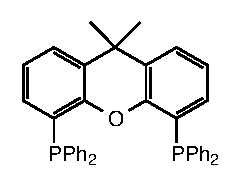
\includegraphics{../Figures/Xantphosderivatives/Phxantphos.eps}
	\caption{\Phxantphos}
	\label{biteanglePhxantphos}
\end{subfigure}
~
\begin{subfigure}[b]{0.3\textwidth}
	\centering
	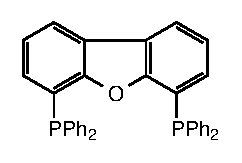
\includegraphics{../Figures/Xantphosderivatives/DBFphos.eps}
	\caption{DBFphos}
	\label{biteangleDBFphos}
\end{subfigure}
\caption[Wide bite-angle diphosphine ligands]{Wide bite-angle diphosphine ligands.}
\label{widebiteanglediphosphines}
\end{figure}

\begin{figure}[htbp]
\centering
\begin{subfigure}[b]{0.3\textwidth}
	\centering
	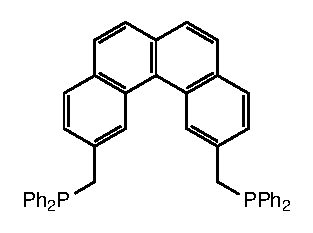
\includegraphics{../Figures/Diphosphines/TRANSphos.eps}
	\caption{TRANSphos}
	\label{TRANSphos}
\end{subfigure}
~~~
\begin{subfigure}[b]{0.3\textwidth}
	\centering
	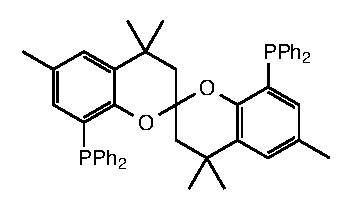
\includegraphics{../Figures/Diphosphines/SPANphos.eps}
	\caption{SPANphos}
	\label{SPANphos}
\end{subfigure}
~~~
\begin{subfigure}[b]{0.3\textwidth}
	\centering
	
\includegraphics{../Figures/Diphosphines/norphos.eps}
	\caption{norphos}
	\label{norphos}
\end{subfigure}
\caption[Trans-spanning diphosphine ligands]{Selected trans-spanning diphosphine ligands.}
\label{transdiphosphines}
\end{figure}

%===========================================================================
\section{Pincer Ligands}

Diphosphine ligands such as \Phxantphos{} with wide bite-angles and a heteroatom in the centre of the backbone have the potential to act as pincer ligands.  Pincer ligands have attracted research attention due to the unique balance of stability and reactivity that they impart on transition metal complexes.\cite{Becerra2009}  Pincer ligands are tridentate ligands that coordinate to transition metals preferentially in a meridional fashion.\cite{Choi2011}   The ligands are typically named according to their donor atoms, such as PCP, POP or NCN (Figure \ref{Pincernaming}).  If the groups between the donor atoms contain heteroatoms then these may be included in the naming also, for example POCOP.  The pincer ligands may be anionic (as with PCP ligands) or neutral (PNP and POP).\cite{Vlugt2009, Kataoka1995}  Although phosphines are the most common donor groups, amines,\cite{Singleton2003} imines,\cite{Takenaka2005} thioethers\cite{Zim2000} and N-heterocyclic carbenes\cite{Hahn2007} have all been reported.

\begin{figure}[ht]
\centering
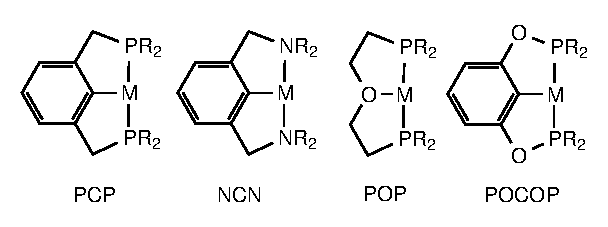
\includegraphics[]{../Figures/Pincernaming.eps}
\caption[Naming of pincer ligands]{Naming of pincer ligands.}
\label{Pincernaming}
\end{figure}

Pincer ligands were first reported in 1976 by Shaw and Alcock.\cite{Moulton1976, Alcock1976}  Shaw reported a \emph{tert}-butyl PCP ligand (Figure \ref{ShawPCP}) and introduced the naming scheme that has become commonplace for pincer ligands.  When reacted with an appropriate metal precursor, complexes of the tridentate ligand formed with nickel, palladium, platinum, rhodium, and iridium with chloride, nitrile, hydride, and carbon monoxide ligands.\cite{Moulton1976}  Alcock reported the first POP pincer ligands together with their rhodium carbonyl complexes, characterised by X-ray crystallography (Figure \ref{AlcockPOP}).\cite{Alcock1976}  

\begin{figure}[htbp]
\centering
\begin{subfigure}[b]{0.3\textwidth}
	\centering
	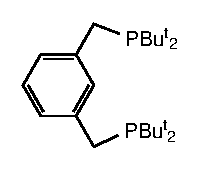
\includegraphics{../Figures/Shaw.eps}
	\caption{}
	\label{ShawPCP}
\end{subfigure}
~
\begin{subfigure}[b]{0.3\textwidth}
	\centering
	
\includegraphics{../Figures/Alcock.eps}
	\caption{}
	\label{AlcockPOP}
\end{subfigure}
\\
\caption[First reported pincer ligands]{First reported pincer ligands.}
\label{Pincerligands}
\end{figure}

The different components of pincer ligands have significant influence on the steric and electronic properties and hence their reactivity.\cite{Singleton2003}  Altering the central donor group, X (Figure \ref{Pincerligands}), can lead to changes in electronic effects mostly through the \trans{}-influence.\cite{Choi2011}  For example, a carbon donor ligand has a greater \trans{}-influence than an oxygen donor.  Thus ligands \trans{} to X in PXP complexes will be bound more strongly when X~=~O than X~=~C.\cite{Zhu2008} The donor group Y controls the steric environment around the metal centre and the electron density.  Changing the backbone and other remote groups gives control over the electron density on the metal and can be used to improve solubility properties.\cite{Choi2011}

\begin{figure}[htbp]
\centering

\includegraphics{../Figures/Pincerligands.eps}
\caption[General representation of pincer complexes]{General representation of pincer complexes.}
\label{Pincerligands}
\end{figure}

The tridentate coordination of pincer ligands, typically forming two five-member\-ed metallacycles, imparts significant stability to metal complexes with pincer ligands.\cite{Choi2011}  The stability of the complexes is such that the backbone can undergo functionalisation at the 4-position \emph{via} lithiation with \emph{tert}-butyllithium and treatment with trimethylchlorosilane, without inducing any decomposition of the platinum complex (Scheme \ref{Stability}).\cite{Albrecht2001}  This inherent stability allows the complexes to act as catalysts for highly endothermic reactions that require high temperatures, such as alkane dehydrogenation.\cite{Choi2011}

\begin{scheme}[htbp]
\centering
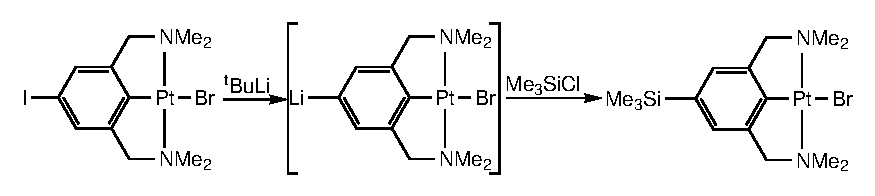
\includegraphics[]{../Schemes/Stability.eps}
\caption[Functionalisation of an NCN pincer ligand]{Functionalisation of an NCN pincer ligand.}
\label{Stability}
\end{scheme}

Coordination complexes of pincer ligands have a large number of applications.  Platinum complexes of an NCN pincer ligand have been utilised as sensors for the detection of sulfur dioxide.\cite{Albrecht2000, Albrecht2000c, Albrecht2001}  Palladium and nickel complexes of a number of pincer ligands have shown activity in cross-coupling reactions.\cite{Hahn2007, Bedford2000, Kimura2006, Zim2000, Obora2006} Theoretical studies have shown potential uses for pincer ligands in water-splitting\cite{Sandhya2011} and nitrogen fixation.\cite{Holscher2007}  However, one of the most prominent uses of pincer ligands is the activation of C-H bonds, typically as dehydrogenation catalysts.\cite{Choi2011, Albrecht2001, Crabtree2001}

%===========================================================================
\section{Xantphos}

First reported in 1995 by van Leeuwen et al., the \acrshort{xantphos}\footnote{The term xantphos is used in the literature to mean either the general class of ligands or the specific ligand 9,9-dimethyl-4,6-bis(diphenylphosphino)xanthene.  For the purposes of this thesis the specific ligand will be referred to as \Phxantphos{} and the term xantphos will be used to represent a generic ligand from this class.} class of diphosphine ligands were designed to investigate the influence of the bite-angle on catalytic reactions, in particular rhodium catalysed hydroformylation.\cite{Kranenburg1995}  The general structure and a selection of different xantphos derivatives are given in Figure \ref{xantphosderivatives}.  The first paper on xantphos included derivatives where the \ce{CMe2} group in the backbone of \Phxantphos{} (Figure \ref{Phxantphos}) was replaced by a S (\Phthixantphos, Figure \ref{Phthixantphos}), \ce{SiMe2} (\Phsixantphos, Figure \ref{Phsixantphos}), a direct bond between the atoms (DBFphos, Figure \ref{DBFphos}), or removed entirely (DPEphos, Figure \ref{DPEphos}).  Since then an vast array of derivatives have been reported.  The most common position for derivatisation is the bridgehead position (occupied by a \ce{CMe2} group in \Phxantphos{}).  Changes to this position can create changes in the natural bite-angles of the ligands.  Another site for derivatisation is the substituents on the phosphorus atoms which have been changed for cyclic groups, chiral derivatives or alkyl chains including methyl, ethyl, isopropyl and \tBu{} groups.  The phosphorus donors have also been replaced with a range of different groups including phosphonites, amines, imines, arsines, and thioethers.\cite{Veen2000b, Malaise2006, Goertz1998, Haaren2002} The third site for derivatisation is the position \emph{meta} to the phosphorus atoms on the backbone phenyl rings.  In \Phxantphos{} this position is occupied by hydrogen atoms, while in \Phthixantphos{} methyl groups are present.  Derivatives with \tBu{} or sulfate groups have also been reported.\cite{Goedheijt1998, Goedheijt1998b, Veen1999}\footnote{In the literature two different structures are commonly referred to as  \tBuxantphos{}, one with \tBu{} substituents on the aromatic backbone and one with \tBu{} groups on the phosphorus atoms.  For the purpose of this thesis the structure with the \tBu{} substituents on the phosphorus will be named \tBuxantphos{} and the structure with the \tBu{} groups on the aromatic backbone will be named \emph{t}-Bu-(\Phxantphos).}  These alterations all result in changes to the bite-angle of the ligand.  

\begin{figure}[htbp]
\centering
\begin{subfigure}[b]{0.35\textwidth}
	\centering
	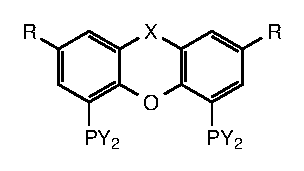
\includegraphics{../Figures/Xantphosderivatives/Generic.eps}
	\caption{General structure}
	\label{genericxantphos}
\end{subfigure}
~
\begin{subfigure}[b]{0.3\textwidth}
	\centering
	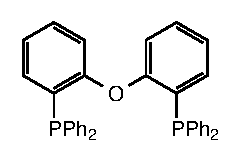
\includegraphics{../Figures/Xantphosderivatives/DPEphos.eps}
	\caption{DPEphos, 102\degrees}
	\label{DPEphos}
\end{subfigure}
~
\begin{subfigure}[b]{0.3\textwidth}
	\centering
	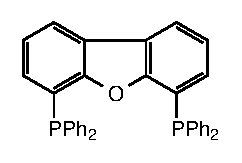
\includegraphics{../Figures/Xantphosderivatives/DBFphos.eps}
	\caption{DBFphos, 131\degrees}
	\label{DBFphos}
\end{subfigure}
\\
\vspace{0.5cm}
\begin{subfigure}[b]{0.35\textwidth}
	\centering
	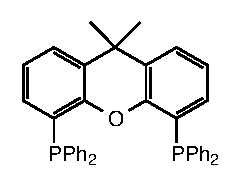
\includegraphics{../Figures/Xantphosderivatives/Phxantphos.eps}
	\caption{\Phxantphos, 111\degrees}
	\label{Phxantphos}
\end{subfigure}
~
\begin{subfigure}[b]{0.3\textwidth}
	\centering
	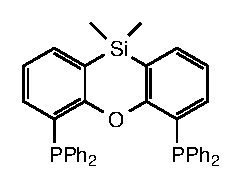
\includegraphics{../Figures/Xantphosderivatives/Sixantphos.eps}
	\caption{\Phsixantphos, 108\degrees}
	\label{Phsixantphos}
\end{subfigure}
~
\begin{subfigure}[b]{0.3\textwidth}
	\centering
	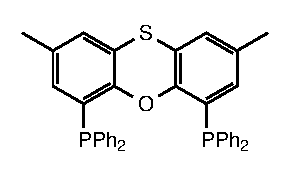
\includegraphics{../Figures/Xantphosderivatives/Phthixantphos.eps}
	\caption{\Phthixantphos, 110\degrees}
	\label{Phthixantphos}
\end{subfigure}
\\
\vspace{0.5cm}
\begin{subfigure}[b]{0.35\textwidth}
	\centering
	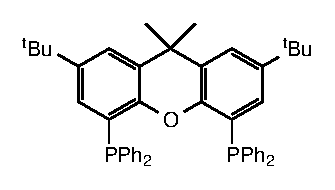
\includegraphics{../Figures/Xantphosderivatives/tBu-Phxantphos.eps}
	\caption{\emph{t}-Bu-(\Phxantphos), 110\degrees}
	\label{tBuPhxantphos}
\end{subfigure}
~
\begin{subfigure}[b]{0.3\textwidth}
	\centering
	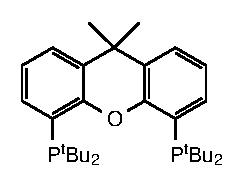
\includegraphics{../Figures/Xantphosderivatives/tBu-xantphos.eps}
	\caption{\tBuxantphos, 140\degrees}
	\label{tBuxantphos}
\end{subfigure}
~
\begin{subfigure}[b]{0.3\textwidth}
	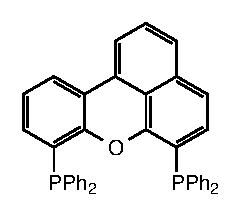
\includegraphics{../Figures/Xantphosderivatives/Benzoxantphos.eps}
	\caption{Benzoxantphos, 120.6\degrees}
	\label{Benzoxantphos}
\end{subfigure}
\\
\vspace{0.5cm}
\begin{subfigure}[b]{0.35\textwidth}
	\centering
	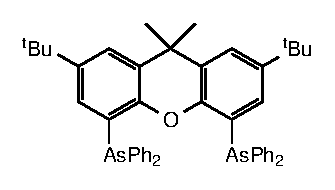
\includegraphics{../Figures/Xantphosderivatives/Xantarsine.eps}
	\caption{Xantarsine, 113\degrees}
	\label{Xantarsine}
\end{subfigure}
~
\begin{subfigure}[b]{0.6\textwidth}
	\centering
	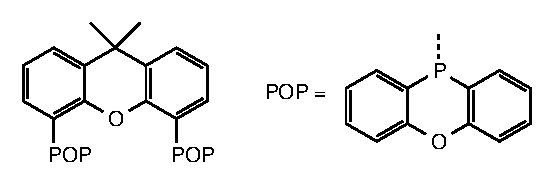
\includegraphics{../Figures/Xantphosderivatives/POP-xantphos.eps}
	\caption{POP-xantphos, 123\degrees}
	\label{POP-xantphos}
\end{subfigure}
\\
\caption[Selection of xantphos derivatives]{Selection of xantphos derivatives with their natural bite-angles (where known).\cite{Dierkes1999, Veen1999, Veen2000, Veen2000b}}
\label{xantphosderivatives}
\end{figure}

The influence of the bite-angle of diphosphine ligands on the selectivity and activity of their transition metal complexes in various catalytic process has been investigated using the xantphos ligands.  The hydroformylation of alkenes to give branched and linear aldehydes is an industrially important reaction with the linear aldehydes typically of higher industrial importance.\cite{Leeuwenbook2000}  In the hydroformylation of 1-octene using various xantphos ligands, a linear correlation was observed between the natural bite-angle of the diphosphine and the percentage of linear aldehyde product.\cite{Kranenburg1995}  From this and other kinetics studies, the bite-angle has been determined to have both a steric and electronic component.\cite{Veen1998, Leeuwen2000}  In hydroformylation the hydride-migration step determines the regioselectivity of the reaction.  In this case additional steric crowding of the metal centre, resulting from a larger bite-angle, can lead to a favouring of the less sterically demanding transition state - that which produces the linear aldehyde.\cite{Freixa2003}  Carrying out the hydroformylation of styrene or 1-octene with a series of thixantphos complexes where the phenyl substituents on the phosphorus atoms were substituted in the \emph{para}-position with various electron donating or electron withdrawing substituents, showed differences in the \gls{TOF} of each reaction.\cite{Veen1998}  This is thought to be related to changes in the metal hybridisation, changing the reactivity of the metal towards reductive elimination.\cite{Slot2002, Freixa2003}

The xantphos ligands were the first tertiary phosphine ligands to form active hydrocyanation catalysts on nickel.\cite{Kranenburg1995b}  Using styrene as a substrate, diphosphines with alkyl backbones, such as \gls{dppe}, \gls{dppp} and \gls{dppb} gave poor yields (\textless{}10\%) where\-as the xantphos ligands gave yields ranging from 27-95\%, with the highest yield for \Phsixantphos{}.  Ligands with bite-angles close to 105\degrees{} resulted in higher yields and selectivities whilst decreasing the bite-angle to 101\degrees{} or increasing to 110\degrees{} led to a much lower activity.  The bite angle can influence the selectivity of the reaction by stabilising preferred reaction intermediates and destabilising inactive species.   In the hydrocyanation reaction a bite-angle close to 109\degrees{} destabilises square-planar Ni(II) species and stabilises the tetrahedral Ni(0) species, enhancing the reductive elimination step and resulting in a faster reaction.\cite{Goertz1998}  The increased reactivity of xantphos complexes compared to other diphosphines including, \acrshort{dppp}, \acrshort{BINAP}, \acrshort{dppf}, and \acrshort{DPEphos} has also been observed in a range of different cross-coupling reactions.\cite{Birkholz2009}

A search of the \gls{CSD} indicates that of the crystallographically determined structures, most complexes with xantphos derivatives involve bidentate \dento{}P,P\textprime{} coordination.\cite{Allen2002}  Four complexes with a 2-coordinate metal centre have been reported, all coordinated to gold. Ten 3-coordinate structures have been published.  With 4-coordinate metals, tetrahedral complexes are the most common (31 structures), followed by pseudo-\trans{} square-planar complexes (26), then \cis{} square-planar geometries (20).  This is particularly interesting as the natural bite-angle of \Phxantphos{} ligands is closer to a 90\degrees{} than to 180\degrees.  On pentacoordinate metals 10 complexes have been reported with one square-pyramidal structure, three axial-equatorial, and six bis-equatorial trigonal bipyramidal complexes found.  Six different octahedral complexes have been reported, all with the xantphos ligand displaying a \cis{}-geometry.  The xantphos ligands can also coordinate in a \POP{} geometry in addition to the bidentate \dento{}P,P\textprime{} mode.  This \POP{} coordination is more common than the \dento{}P,P\textprime{} in octahedral complexes with 24 reported.  However, it is much less common in five coordinate complexes with only four \POP{} complexes and 10 \POP{} four-coordinate complexes.  A monodentate \dento{}P bonding mode is also possible, though it is very rare, with only one crystal structure reported to date.\cite{Escalle2009}

%\fixme{For the above, do I need to cite the actual papers or is citing the CSD enough?}

Given the possibility of \POP{} and \dento{}P,P\textprime{} coordination the xantphos ligands also have the potential for hemilability of the central donor group whereby the oxygen can bind reversibly to the metal centre in order to stabilise catalytic intermediates. This has been utilised in the hydroacylation of alkenes and alkynes using a rhodium pincer complex, where the oxygen can bind in order to stabilise important intermediates and prevent the competing decarbonylation reactions from occurring.\cite{Moxham2006, Moxham2008, Pawley2010}  A range of rhodium complexes with \Phxantphos{} or \gls{DPEphos} as ancillary diphosphine ligands were tested for the hydroacylation reaction.\cite{Moxham2006}  The \gls{DPEphos} complexes were more active than the \gls{dppe} complex used for comparison, achieving conversions of 100\% after 30 min and 90 min respectively.  However, the \Phxantphos{} complex was completely inactive.  The lower reactivity is thought to be a result of the increased rigidity of the \Phxantphos{} backbone compared to that of DPEphos.\cite{Pawley2010}

\subsection{Alkyl-Substituted Xantphos Ligands}

Despite the large number of xantphos derivatives few examples of xantphos ligands with alkyl substituents on the phosphorus atoms have been reported.  The synthesis and some coordination chemistry of xantphos ligands with methyl, ethyl, isopropyl, and \tBu{} substituents has been studied.  Me-xantphos was reported in 2002 and investigated for reactivity with \ce{[Pd(cod)ClMe]} (\acrshort{cod} = \acrlong{cod}), to produce \cis-[PdCl(Me-xantphos)Me].\cite{Zuideveld2002}  The \cis{} isomer was also formed using \Phsixantphos.  However, using the larger bite-angle ligands \Phthixantphos{} and \Phxantphos{} \cis-\trans{} isomerism was observed at room temperature.  Reaction of the four chloridomethyl complexes with \ce{AgSO3CF3} yielded the pincer complexes [PdMe(xantphos-\POP)]\ce{[SO3CF3]} (Scheme \ref{Pdchloromethyl}).  

\begin{scheme}[htbp]
\centering
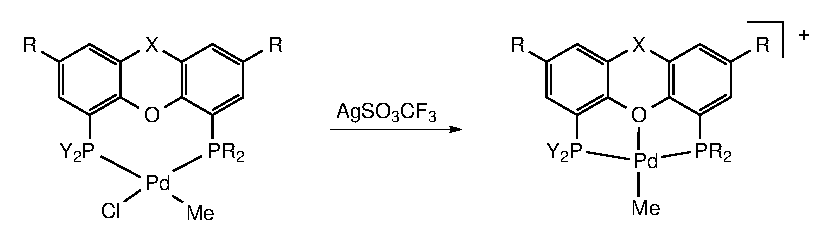
\includegraphics{../Schemes/Pdchloromethyl.eps}
\caption[Chloride abstraction from [PdClMe(xantphos){]}]{Chloride abstraction from [PdClMe(xantphos)] xantphos = \Phsixantphos{}, \Phthixantphos{}, \Phxantphos{}, and Me-xantphos.}
\label{Pdchloromethyl}
\end{scheme}

A variant of xantphos with ethyl groups on the phosphorus atoms (Et-xantphos) was reported in 2004.\cite{Miedaner2004, Raebiger2004}  Palladium and platinum complexes, [M(Et-xantphos\ce{)2}], [M(Et-xantphos\ce{)2]^{2+}} and platinum complexes [Pt(Et-xantphos\ce{)2H]PF6} and [Pt(Et-xantphos\ce{)2(H)2]^{2+}} have been studied for their electrochemical properties.  The X-ray crystal structures of [M(Et-xantphos\ce{)2}] (M = Pd, Pt) were obtained and have a tetrahedral geometry, with average bite-angles of 108.3\degrees{} for both metals.  The palladium(II) complex had two molecules in the unit cell, one closer to a square-planar geometry (average bite-angle = 139.7\degrees) and the other closer to a tetrahedral geometry (average bite-angle = 95.8\degrees).  The pseudo-square planar [Pd(Et-xantphos\ce{)2](BF4)2} complex was also crystallised, and had much larger bite-angles than any of the other ethyl substituted diphosphines included in the study (\gls{depp}, \gls{depx} and \gls{depPE}) indicating the ability of the xantphos ligands to support metals in unusual geometries.  

A xantphos ligand with isopropyl substituents on the phosphorus atoms, \iPrxantphos{}, was first reported in 2010, together with the osmium complex [Os(\iPrxantphosk)\ce{Cl3}], showing the \POP{} coordination which is common for xantphos ligands in octahedral complexes.\cite{Asensio2010}  The same research group, has since investigated the synthesis and reactivity of [M\ce{Cl2}(DMSO-\dento{}S)(\iPrxantphos)] (M = Os, Ru) producing a number of different osmium and ruthenium complexes including various polyhydrides and bis(alkynyl)vinylidene complexes.\cite{Alos2013, Alos2014}  

A study of the reactivity of \iPrxantphos{} towards palladium shows differences to the \Phxantphos{} ligand.\cite{Bakhmutov2012}  The [Pd(\ce{CF3})Ph(\Phxantphos)] complex exists in a \cis{} geometry in the solid state, and as \cis{} and \trans{} isomers in solution, whereas the analogous \iPrxantphos{} complex shows only a \trans{} configuration.  The \iPrxantphos{} complex was synthesised in a different manner as the \Phxantphos{} ligand was readily displaced by \ce{CF3-} from \ce{CF3SiMe3}/\ce{F-} while the \iPrxantphos{} ligand was not, indicating the different chemistry of the two ligands.  The difference in the coordination geometries also meant that the \ce{PhCF3} was more readily lost from the \cis-[Pd(\ce{CF3})Ph(\Phxantphos)] than the \trans-[Pd(\ce{CF3})Ph(\iPrxantphos)].  A related study investigated nickel complexes of \iPrxantphos{} for the trifluoromethylation of aryl halides.\cite{Jover2014}  The [NiF(1-naphthyl)(\iPrxantphos)] complex reacted with \ce{CF3SiMe3} forming [Ni(\ce{CF3})(1-naphthyl)(\iPrxantphos)].  Both of these complexes were found to have \trans{}-geometries through X-ray crystallography, and showed slow decomposition at 140 \degC{} and 120 \degC{} respectively, giving rise to a range of products, with no C-F compounds or 1-trifluoromethyl-naphthyl formed.  

The chemistry of rhodium and iridium complexes with \iPrxantphos{} have also been studied.  Reaction of \iPrxantphos{} with [Rh(coe\ce{)2(\hapto{}-Cl)]2} (\acrshort{coe} = \acrlong{coe}) generated the [RhCl(\iPrxantphosk)] complex cleanly.\cite{Esteruelas2013}  However, reaction with the iridium analogue resulted in cyclometallation of one of the isopropyl groups  forming [IrClH(\iPrxantphos-\dento{}-C,P,O,P\textprime].  The chloride ligand in [RhCl(\iPrxantphosk)], was replaced with a hydride, \emph{via} reaction with \ce{KO^{i}Pr}, producing KCl and acetone as by-products.  The trihydride [Ir(H\ce{)3}(\iPrxantphosk)] was produced by reaction of the metallated iridium complex with KOH and \ce{^{i}PrOH}.  The rhodium chloride complex readily splits hydrogen to form [RhCl(H\ce{)2}(\iPrxantphosk)].  The analogous iridium complex was synthesised by reaction of the metallated complex with \emph{n}-octane at 90 \degC.  Recent research has shown that the chloride can be removed from [RhCl(H\ce{)2}(\iPrxantphosk)] by reaction with \ce{Li[B(C6F5)4]OEt2} forming [Rh\ce(H\ce{)2}(\iPrxantphosk)\ce{]+}.\cite{Haibach2013}  The reaction of [RhCl(\iPrxantphosk)] and [IrClH(\emph{i}-Pr-xantphos-\dento{}-C,P,O,P\textprime] with triflic acid results in [MCl(H)(OTf)(\iPrxantphosk)] (M = Rh, Ir).\cite{Esteruelas2013}  The reactivity of the \iPrxantphos{} complexes is summarised in Figure \ref{RhiPrxantphos} and \ref{IriPrxantphos} for rhodium and iridium respectively.  

\begin{scheme}[htbp]
\centering
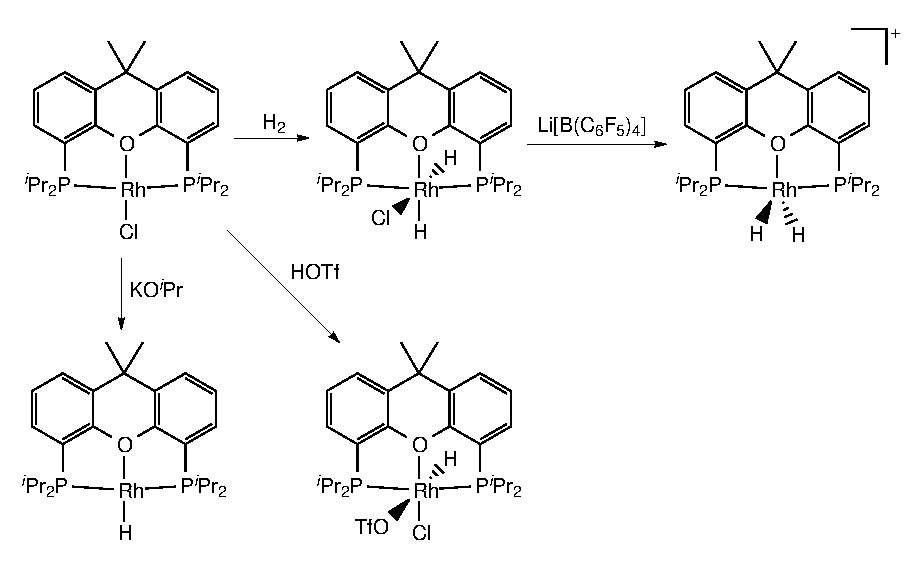
\includegraphics{../Schemes/RhiPrxantphos.eps}
\caption[Reactions of [Rh(\iPrxantphos){]}]{Reactions of [Rh(\iPrxantphos){]}.}
\label{RhiPrxantphos}
\end{scheme}

\begin{scheme}[htbp]
\centering
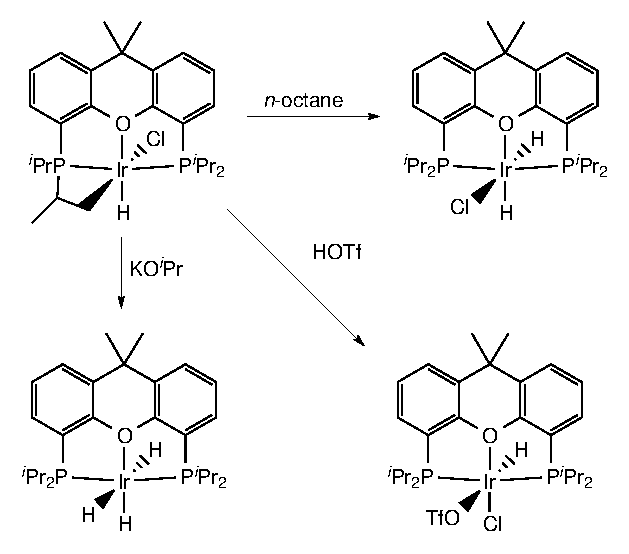
\includegraphics{../Schemes/IriPrxantphos.eps}
\caption[Reactions of [Ir(\iPrxantphos){]}]{Reactions of [Ir(\iPrxantphos){]}.}
\label{IriPrxantphos}
\end{scheme}

The reactivity of the rhodium and iridium complexes towards silyl compounds has also been investigates with the results summarised in Figure \ref{IrRhsilyl}.\cite{Esteruelas2013b}  Reaction of [RhCl(\iPrxantphosk)] or [IrClH(\iPrxantphos-\dento{}-C,P,O,P\textprime] with \ce{SiH2Ph2} or \ce{SiHEt3} resulted in [MCl(H)(\iPrxantphosk)(Si\ce{R3})] (M = Rh, Ir. \ce{SiR3} = \ce{SiHPh2}, \ce{SiEt3}).  The diphenylsilane complexes were unstable in solution converting to [Rh(Si\ce{ClPh2})(\iPrxantphosk)] \emph{via} loss of molecular hydrogen and \trans{}-[Ir(Si\ce{ClPh2)(H)2}(\iPrxantphosk)].  The rhodium complex [RhH(\iPrxantphos)] also underwent reaction with \ce{SiHEt3} and \ce{SiHPh3} initially forming the dihydride [Rh(H\ce{)2}(\iPrxantphosk)\ce{(SiR3)}] (R = Et, Ph) which loses molecular hydrogen to form [Rh(\iPrxantphosk)(Si\ce{R3})].  Reaction of [Rh(Si\ce{ClPh2})(\iPrxantphosk)] with \ce{NaBAr^{F}4} in the presence of water produced [Rh(H)(\iPrxantphosk)(\ce{SiOHPh2})] which was tested as a catalyst for the alcoholysis of \ce{SiH2Ph2} with various alcohols in toluene at 32 \degC, forming ROSiH\ce{Ph2} in isolated yields of 71 - 92\% with \glspl{TOF} of 4000 to 76500 \si{\per\hour}.

\begin{scheme}[htbp]
\centering
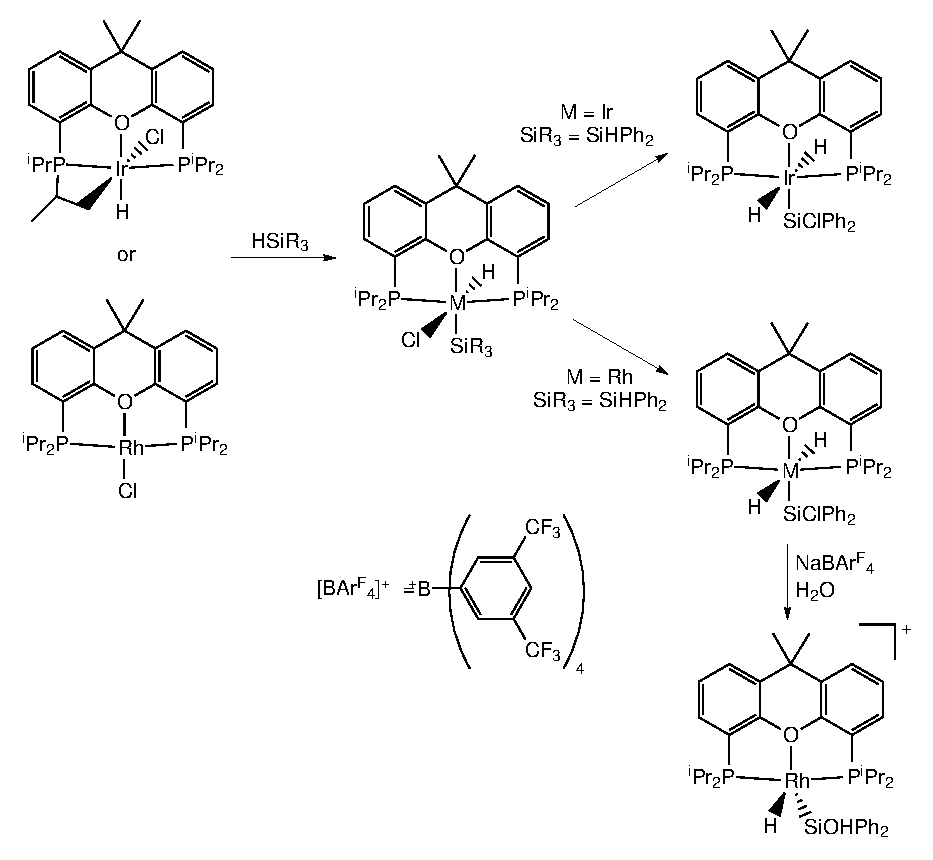
\includegraphics{../Schemes/RhIrsilyl.eps}
\caption[Reactions of Rh and Ir \iPrxantphos{} complexes with silanes]{Reactions of Rh and Ir \iPrxantphos{} complexes with silanes. \ce{SiR3} = \ce{SiHPh2}, \ce{SiEt3}.}
\label{IrRhsilyl}
\end{scheme}

\subsection{\tBuXantphos}

This thesis covers an investigation into the coordination chemistry of three different xantphos ligands with \tBu{} substituents on the phosphorus atoms.  The three ligands differ in the bridgehead position: \tBuxantphos{} has \ce{CMe2}, \tBusixantphos{} has \ce{SiMe2} and \tButhixantphos{} has a thioether bridge.  The first mention of \tBuxantphos{} was in 2002 with the unsuccessful attempts to synthesise \tBuxantphos{} from either the dilithiated backbone or 9,9-dimethyl-4,5-bis(dichlorophosphino)xanthene, the researchers postulated that steric crowding was the reason for the lack of reactivity.\cite{Zuideveld2002}  A successful synthesis of \tBuxantphos{} from the dilithiated backbone was reported in 2005 using heptane as a solvent and heating the reaction mixture to 60\degC{}.\cite{Mispelaere2005}  \tBuXantphos{} has subsequently been studied for use as an ancillary ligand in the palladium catalysed cross-coupling of thiols and aryl bromides or triflates, the iron catalysed \ce{sp^3}-\ce{sp^3} cross-coupling of alkyl halides with alkyl Grignard reagents, the platinum catalysed amination of allylic alcohols and the N-arylation of heterocyclic diamines, all with poor yields, while higher yields were observed when \Phxantphos{} was used.\cite{Mispelaere2005, Dongol2007, Ohshima2009, Cabello2007}  These studies have focussed on the addition of \tBuxantphos{} as a component of the catalytic system.  Few complexes of \tBuxantphos{} have been characterised, although the difference in the catalytic results suggest differences in the coordination chemistry of \Phxantphos{} and \tBuxantphos{}.  

%All of these studies used catalysts formed in \emph{situ}, so the coordination chemistry was not investigated, although the reactivity suggests differences in the coordination chemistry of \Phxantphos{} and \tBuxantphos{}, warranting further investigation.

Prior to the start of this research, the only isolated coordination complexes of \tBuxantphos{} were [Au(\tBuxantphos)][\ce{AuX2}] (X = Cl, Br, I), formed by reaction of [AuCl(\acrshort{tht})] (\acrshort{tht} = \acrlong{tht}) with \tBuxantphos{} and subsequent reaction with KBr or KI.\cite{Partyka2010}  The analogous reaction using \Phxantphos{} gave [(AuX\ce{)2}(\Phxantphos)] (X = Cl, Br, I) with each phosphorus atom coordinated to a separate gold centre with a Au-Au interaction.\cite{Pintado2004, Partyka2010}  Subsequent investigations into the catalytic activity of gold xantphos complexes towards the C-F bond activation of perfluoroarenes showed \glspl{TON} of 200 for [AuCl(\Phxantphos)] and 1000 for [Au(\tBuxantphos)][\ce{AuCl2}].\cite{Zhan2012}  Mechanistic studies into the reaction showed that [Au(xantphos)\ce{]+} was an important intermediate and is in equilibrium with the inactive [Au(xantphos\ce{)2}].  Due to the size of \tBuxantphos{} the equilibrium favours the two-coordinate species while for \Phxantphos{} the four-coordinate complex is preferred, resulting in lower activity.\cite{Zhan2012}  This clearly shows the difference between the two xantphos ligands and suggests that a difference in the coordination chemistry may be the reason for the lack of catalytic reactivity in the \tBuxantphos{} systems.  

Subsequent to the start of the research presented in this thesis \tBuxantphos{} has gained increasing attention, likely as a result of the ligand becoming commercially available.  In the six years 
from the first successful synthesis in 2005 to the start of this research in mid-2011, only the four papers discussed above were published investigating \tBuxantphos{}.\footnote{Two papers investigating the use of the dioxidised \tBuxantphos{} as a ligand on europium and samarium were also published in 2011 and 2012.\cite{Miyata2011, Miyata2012}}  However, the following three years showed increasing attention with 9 papers published\cite{Friis2014, Dang2013, Liu2013c, Raoufmoghaddam2013, Haibach2013, Ashcroft2013, Behr2013, Raoufmoghaddam2013b, Zhan2012} and 10 patent applications.\cite{Shang2010, Shang2011a, Shang2011b, Shang2011c, Shang2012a, Brandstadt2013a, Brandstadt2013b, Brandstadt2013c, Brandstadt2013d, Brandstadt2013e}

Further investigations into the catalytic properties of \tBuxantphos{} have been reported, without investigation into the coordination chemistry.  These include the  palladium-catalysed cross-coupling of 2-(4-bromophenyl)-5-chloropyrazine with a benzimidazole boronic ester and hydroesterification of methyl oleate.\cite{Ashcroft2013, Behr2013} In both cases little conversion was observed when \tBuxantphos{} was used, though the \Phxantphos{} systems showed significant reactivity.  The aminocarbonylation of aryl bromides was performed with each of \Phxantphos{} and \tBuxantphos{} in an unusual monodentate coordination mode.\cite{Friis2014}  Little reactivity was observed with \tBuxantphos{}, while the \Phxantphos{} system gave the product in 92\% isolated yield.  In the rhodium catalysed reductive amination of aldehydes \tBuxantphos{} showed a 59\% total conversion with only 19\% selectivity for the desired product, while \Phxantphos{} had an 84\% conversion and 93\% selectivity.\cite{Raoufmoghaddam2013}   

In some cases the \tBuxantphos{} system is more active than the \Phxantphos{} system, such as the palladium catalysed N-alkylation of aniline with benzyl alcohol.\cite{Dang2013} The \tBuxantphos{} system showed near quantitative conversion at 100 \degC{} while the \Phxantphos{} system showed only 63\% conversion at 110\degC{}.  Improved activity with \tBuxantphos{} compared to \Phxantphos{} was also observed in the palladium catalysed methylation of alkynyl C-H bonds with dimethyl sulfonium ylides.\cite{Liu2013c}  Under the same conditions a yield of 46\% was obtained with \tBuxantphos{} while only 15\% was produced using \Phxantphos{}.  \tBuXantphos{} and \Phxantphos{} can also have similar results, such as in the rhodium catalysed hydroamidomethylation of 1-pentene with acetamide, \Phxantphos{} and \tBuxantphos{} showed conversions of 83 and 80\% respectively with greater than 99\% linearity in both cases.\cite{Raoufmoghaddam2013b}  

Despite the increased interest in \tBuxantphos{} in the last four years, research has focussed on its use as an ancillary ligand for catalytic reactions, mostly with the catalyst formed \emph{in situ}.  A crystal structure of \trans-[Pd(\tBuxantphos)\ce{Cl2}], was reported \emph{via} communication to the \gls{CSD} in 2011 (CSD-XARXAR), no further publication of this complex has followed.\cite{Allen2002}  One paper has reported the coordination behaviour of the \tBuxantphos{} ligand with rhodium.\cite{Haibach2013}  Similarly to the work with \iPrxantphos{}, the \tBuxantphos{} ligand reacts with [Rh(\acrshort{coe})(\hapto{}-Cl)\ce{]2} (\acrshort{coe} = \acrlong{coe}) to give [Rh(\tBuxantphosk)Cl].  This Rh(I) chloride can readily split hydrogen to form a [Rh(\tBuxantphosk)Cl\ce{(H)2}] complex.  The structures of [Rh(\tBuxantphosk)Cl] and [Rh(\tBuxantphosk)Cl\ce{(H)2}] have been confirmed by X-ray crystallography.  Chloride abstraction from [Rh(\tBuxantphosk)Cl\ce{(H)2}] using \ce{AgBF4} or \ce{AgSbF6}, generates the trigonal bipyramidal complex [Rh(\tBuxantphosk)\ce{(H)2}], with the \tBuxantphos{} ligand retaining the meridional coordination typical of pincer ligands.  This dihydride was found to react with ethene to give ethane and [Rh(\tBuxantphosk)(\ce{C2H4})], however no reaction with the commonly used hydrogen acceptors, \emph{t}-butylethylene or norbornene, was observed, nor was any reaction with terminal alkenes.  [Rh(\tBuxantphosk)Cl\ce{(H)2}] reacts with \ce{KO^{t}Bu} resulting in a four-coordinate mono-hydride species [Rh(\tBuxantphos)H].  Addition of ethene to [Rh(\tBuxantphos)H] resulted in the reversible formation of an ethyl complex.  The [Rh(\tBuxantphos)H] complex also showed reactivity in the isomerisation of 1-hexene with a \gls{TON} of 2000 after 16 hours.  

The previous work exploring \tBuxantphos{} and \Phxantphos{} as ancillary ligands for catalytic processes has shown significant differences in the yields of the reactions in most cases, though in one case a similar activity was reported.  Although a number of palladium catalysed reactions have been studied, only two palladium complexes have been reported (one being only a crystal structure).  The only research into the coordination chemistry of the \tBuxantphos{} ligands is on gold and rhodium.\cite{Partyka2010, Haibach2013}  The original study into the xantphos ligands focussed on changing the bridging groups of \Phxantphos{} showing the impact that subtle changes in the bite-angle can have on the catalytic activity of the transition metal complexes.\cite{Kranenburg1995}  Given the number of studies investigating the catalytic activity of \tBuxantphos{} without investigating the coordination chemistry, an examination of the coordination chemistry of a range of subtly different \tBuxantphos{} ligands with late-transition metals is of particular interest.   

%===========================================================================
\section{Research Objectives}

The xantphos class of ligands has been the subject of a number of studies, with interesting and varied results.  The initial research with \Phxantphos{} investigated the influence of changes in the bite-angle resulting from changing the group in the bridging position from the \ce{CMe2} group found in \Phxantphos.\cite{Kranenburg1995, Kranenburg1998, Kamer2001}  These studies have shown that small changes in the bite-angle can have a significant impact on the catalytic reactivity and selectivity of the system.  Recently a large amount of research has focussed on the development of xantphos derivatives with alkyl substituents on the phosphorus atoms, particularly the \iPrxantphos{} and \tBuxantphos{} ligands.  Prior to the start of this research only one report investigating the coordination behaviour of \tBuxantphos{} had been published.\cite{Partyka2010}  The other studies all showed much lower activity in catalytic systems than with the \Phxantphos{} ligand.\cite{Ohshima2009, Mispelaere2005, Dongol2007}   Together this suggested that the coordination behaviour of the \tBuxantphos{} and \Phxantphos{} ligands is different and deserved further attention.  The papers published since the inception of this research have only sought to solidify the objectives, as these have reported several examples of studies into the use of \tBuxantphos{} in catalytic systems with only one further study into the coordination behaviour on rhodium, despite the majority of the catalytic studies being performed on palladium.  Furthermore, despite the much larger bite-angle and the electronic differences of \tBuxantphos{} compared to \Phxantphos, and the impact small bite-angle changes have on the activity of \Phxantphos{} only two xantphos ligands with \tBu{} substituents on the phosphines and \ce{CMe2} or \ce{C=CMe2} in the bridgehead position have been published, and no comparative investigation has been reported.

The over-arching goal of this research is to investigate the synthesis, properties and coordination chemistry of \tBuxantphos{} and two derivatives in the bridgehead position (S and \ce{SiMe2}).  The first stage will aim to synthesise the \tButhixantphos{} and \tBusixantphos{} ligands, and investigate the steric and electronic properties of all three \tBuxantphos{} ligands by the calculation of their natural bite-angles and synthesis of some non-transition metal derivatives.  

Silver is a particularly interesting metal for the synthesis of coordination complexes, showing a distinct propensity to form dimers, trimers, or higher order structures, with differences dependent upon the steric bulk and flexibility of the diphosphine ligands used.\cite{Meijboom2009}  Hence, the initial coordination chemistry of the three \tBuxantphos{} ligands towards silver will be investigated in order to gain an understanding of their coordination chemistry and gauge the impact of their large bite-angles on the coordination chemistry, and to allow comparison to the gold \tBuxantphos{} complexes previously published.

The remainder of the research will focus on transition metals which are commonly used in homogeneous catalysis.  The xantphos class of ligands have been well-studied for their roles as ancillary ligands in hydroformylation.\cite{Veen1998, Veen1999b, Veen2002, Zuidema2008, Petocz2004, Bronger2003, Kranenburg1995}  The aim of this research is not to investigate the catalytic properties of the three \tBuxantphos{} ligands, but to produce discrete transition metal complexes to gain insight into the catalytic studies that have already been performed.  Hence the coordination chemistry with rhodium will focus on the synthesis of a simple rhodium(I) complex and establish the reactivity towards small molecules, including hydrogen and carbon monoxide, which are the foundation for a number of different catalytic processes.  

The coordination chemistry of the three \tBuxantphos{} ligands towards palladium and platinum in both the 0 and +2 oxidation states will also be studied, in order to gain insight into the differences in the catalytic activity of systems with \tBuxantphos{} and \Phxantphos{}.  Palladium is one of the most widely used metals for homogeneous catalysis and catalytic cycles frequently involve interconversion between the two oxidation states.\cite{Tsuji1995}  Platinum complexes will be synthesised prior to the palladium investigation as the presence of an NMR active isotope (\Pt) coupled with the high stability of platinum complexes can be beneficial to the identification and characterisation of any complexes produced.  Although the coordination chemistry of \Phxantphos{} with palladium is well-known, few coordination complexes of \Phxantphos{}, and particularly \Phthixantphos{} and \Phsixantphos{} with platinum have been reported.  This work will begin with a brief investigation into the coordination chemistry of \Phthixantphos{} with platinum to assist in identifying any differences in the coordination chemistry that may result from changing the phenyl substituents to \tBu{} groups.  The coordination chemistry of the three \tBuxantphos{} ligands with palladium and platinum in the 0 and +2 oxidation states will then be performed.

Throughout this research \gls{NMR} spectroscopy will be used extensively to characterise the products of the reactions and aid in the identification of any intermediates or dynamic processes that may be present.  X-ray crystallography will also be an important tool, particularly to compare the bite-angles and coordination geometries of the \tBuxantphos{} complexes produced with those previously reported for the \Phxantphos.  \Gls{DFT} will also be used to gain further insight into reactions or processes when this is beneficial.


%\section{Tertiary Phosphine Ligands}
%
% They are very widely used in a range of catalytic transformations as ancillary ligands.  Bonding through the donation of the lone pair on the phosphorus atom, tertiary phosphines are considered strong sigma-donors and \fixme{pi}-acceptor ligands.  The strong bond that forms as a result of the donation from the phosphorus to the metal combined with back-donation from the metal centre \fixme{is there really back-donation?} allows tertiary phosphine ligands to bond very strongly to the metal.  This strong bond imparts a great deal of stability to the complexes allowing longer lifetimes in catalytic transformations, resulting in higher turnover numbers (TON, the maximum number of turnovers that a single molecule of catalyst can perform before degradation).  Similarly to other common ligands like N-heterocyclic carbenes (NHC) the tertiary phosphine ligands impart a great deal of control over the metal centre.
%
%The tertiary phosphine ligands can be derivatised in a number of different ways to change the properties of the phosphine.  Unlike NHC ligands which typically have an imidazolium core, which means that derivatisation occurs further away from the coordinating atom, tertiary phosphines can be derivatised directly in the alpha position meaning that changes have a much greater impact on the metal centre, thus affecting its reactivity and selectivity in a range of different ways, hence having a great impact on the different catalytic processes that a metal may undertake.
%
%Tertiary phosphines are typically used in catalytic transformations as ancillary ligands.  Ancillary ligands are ligands that are not directly involved in the catalytic process (though they may \fixme{de-ligate} and then re-coordinate to allow for free coordination sites for the catalytic reagents).  However, ancillary ligands can impart a great deal of control over the reaction taking place.  Changing the ligand to a different ligand may result in different regio- or stereoselectivity, or it may change the nature of the product entirely (polyketone rather than methyl methacrylate for dbpx reaction).  Furthermore changing the ligand may have a dramatic effect on the nature of the product and the rate of reaction.  As previously discussed the phosphine imparts a great deal of stability to the metal centre meaning higher turnover numbers.  Catalysis is a fine balance between meeting the stability requirements so the catalyst undergoes a large number of turnovers before degrading and ensuring that there is enough instability in the system so that it isn't a rock and actually loses some ligands to form free coordination sites for the catalyst to coordinate to and that the resulting "resting state" is unstable enough so that it progresses through the catalytic cycle.  
%
%Altering the groups coordinated to the phosphorus can also change the steric and electronic environment around the metal centre.  A number of asymmetric ligands such as BINAP and CAMP are chiral ligands used in asymmetric catalysis such as the synthesis of L-dopa an important drug used in the treatment of Parkinson's disease.  These ligands are able to control the steric environment around the metal centre such that the substrate will prefer to coordinate to a particular site or in a specific geometry thus allowing chirality to be introduced in the product.  This is one important application for asymmetric catalysis.  However, there are a number of different ways in which the steric bulk of a system may impact the catalytic transformation.  For example, a non-chiral but sterically bulky ligand may result in coordination of different combination of substrates by selectively allowing coordination at the terminal of a molecule rather than in the middle of a chain.  For polymerisation of ethene this may result in linear chains, thus forming high density polyethylene rather than the branched low density products.  For other reactions sterically bulky ligands may enhance certain geometries of transformations.  For example an alkyl migration may occur more favourably to form a linear rather than branched product.  This is important for a number of reactions such as hydroformylation or other carbon-carbon reactions involving alkenes such as hydroesterification, allylic alkylation or alkoxycarbonylation.  Using sterically bulky phosphines as ancillary ligands can also prevent side-reactions occurring leading to large distributions in the products.
%
%Large sterically bulky ligands can also promote a number of different steps that occur in catalytic transformations.  Frequently the rate-determining-step involves the coupling of two ligands in a reductive elimination.  As such, the presence of large ligands which restrict the space around the metal centre can enhance the speed with which this occurs generally by destabilising the starting intermediate \fixme{the thing before it has reductively eliminated}.  The sterically bulky ligands can also reduce the degradation pathways by preventing the formation of inactive materials such as by having two of the same substrate coordinate to the metal.  They can also reduce the likelihood of degradation from molecules such as oxygen or nitrogen coordinating to the metal centre.  
%
%\subsection{Electronic and Steric Parameters}
%
%Attempts have been made to quantify the steric and electronic nature of tertiary phosphine ligands.  
%In order to analyse and compare the electronic properties of tertiary phosphine ligands an indirect measure of their donor ability is required.  %
%\section{Diphosphine Ligands}
%
%Diphosphine ligands are ligands that consist of two tertiary phosphine groups linked by some sort of backbone.  Most typically this takes the form of a carbon skeleton such as an ethyl, propyl or xylyl group as found in 1,2-\emph{bis}-diphenylphosphinoethane (dppe), 1,2-\emph{bis}-diphenylphosphinopropane (dppp) or dbpx \fixme{what is dbpx's full name?}.  Some more unusual backbones include the pyridyl backbone found in a number of pincer ligands, and a ferrocene molecule such as that found in diphenylphosphinoferrocene (dppf).  Diphosphines are particularly interesting molecules as having two phosphorus donor ligands joined through a backbone allows further control over the geometry of the coordination complex.  This additional control can be displayed through changes in the reactivity, selectivity and regioselectivity of various different catalytic transformations.  Diphosphines are able to exert more control over the metal centre and as such they can have dramatic changes to the reactivity compared to a catalyst comprised of two monophosphine analogues.  
%
%The additional stability of diphosphine complexes is a result of the chelate effect.  During catalysis it is quite common for the metal complex to lose ligands in order to form free coordination sites in order for the substrates to coordinate and thus allow the catalytic transformation to take place.  For monophosphine ancillary ligands frequently the ligand is lost and then needs to compete for the free coordination site with the substrates once the reaction is complete.  This can lead to significant degradation of the catalyst and is generally overcome by addition of some free phosphine ligand.  However, the phosphine is still generally not the major component of the reaction mixture as doing so may result in complexes that are coordinatively saturated with the phosphine ligand and henceforth display reduced reactivity.  For a diphosphine ligand, if one arm of the ligand has dissociated in order to make room for the substrate molecules, the diphosphine ligand is still connected to the metal centre through the other arm of the diphosphine.  This holds the uncoordinated arm in close proximity to the metal centre and thus increases the effective concentration of the ligand from the perspective of the metal.  This chelate effect is an entropic effect which supposes the intramolecular reactions are always preferred over intermolecular reactions as intermolecular reactions have a decrease in the overall entropy of the transformation (i.e. two molecules continue as two individual molecules rather than the two molecules reacting to form a single entity).  Overall this has the effect of maintaining the disorder (number of molecules) in the system rather than decreasing it as would happen if another substrate coordinated rather than the other arm coming back in.
%
%In square planar and octahedral complexes diphosphine ligands typically occupy a \cis{} geometry while the analogous monophosphines frequently have a thermodynamic driving force to form the \trans{} isomer.  This locking-in of a \cis{} geometry means that the catalyst should remain in a \cis{} form throughout a catalytic process.  This means that a common degradation pathway - namely the isomerisation to a \trans{} complex - is avoided through the use of a chelating disphosphine.  This can enhance the turnover numbers and even the turnover frequency as isomerisation is not a possibility.  Numerous catalytic process exist where changing from monophosphines to a diphosphine has altered not only the reactivity by also the selectivity of a reaction.  In addition having a chelating ligand imparts further stability on a complex without affecting it's reactivity \fixme{lies?} this means that the diphosphine complex may be able to undergo more turnovers before degrading, thus resulting in a higher yield from the catalytic reaction.  In addition one of the phosphorus atoms may be able to \fixme{de-ligate} and form a free coordination site enabling the catalytic cycle to progress while still imparting the stability that comes from having a phosphine ligand.  In addition once the reaction has progressed and the coordination site is no longer needed the phosphine is held in close proximity to the metal such that this arm of the diphosphine is more likely to recoordinate and reform the catalyst resting state rather than another molecule of substrate coordinating and potentially leading to catalyst degradation.  
%
%Trigonal bipyramidal structures are very common intermediates for catalytic transformations, especially those involving rhodium like hydroformylation.  In these complexes diphosphine ligands can typically coordinate in two different geometeries.  Namely a \emph{bis}-equatorial complex or an axial-equatorial mode.  There is a further possibility of a \emph{bis}-axial mode.  However, this is unlikely as the equatorial ligands will impose steric restrictions on the diphosphine ligand preventing it from forming a \emph{bis}-axial complex.  It is quite common to switch between octahedral, trigonal bipyramidal, square-planar or tetrahedral complexes in a catalytic cycles.  Each of these can form a number of different isomers.  If a ligand is able to exert steric or electronic restrictions on the metal geometry that can form then some of these will be more or less favoured from a thermodynamic or kinetic perspective.  This means that the diphosphine ligand can control the geometry of the intermediates and thus control the manner in which the reactions proceeds, thereby control the product distribution and potentially altering the regioselectivity and stereoselectivity of a system.  This may also have a significant impact on both the turnover number (if the diphosphine can promote stable complexes) and the turnover frequency. 
%
%In a similar manner to monophosphine ligands, diphosphine ligands can be described using the electronic parameters described earlier.  However, in there are a few minor differences.  Namely, as discussed previously, diphosphine ligands typically coordinate in a \cis{} geometry, this means that the series are not directly comparable as there will be an effect from the different geometries.  This is most prominent in the rhodium series of \ce{[Rh(CO)ClL2]} complexes as one of the phosphorus atoms will be \trans{} to a carbonyl while the other will be \trans{} to a chloride ligand.  The parameters determined by NMR spectroscopy will be most affected by this as the \trans{} influence has a large effect on the coupling constants.  In the \ce{[PtCl2(monophosphine)2]} and the \ce{[Rh(CO)Cl(monophosphine)2]} complexes the electronic properties of the ligands were able to be determined as the ligand was \trans{} to an identical phosphine.  However, when using a diphosphine the most likely geometry is a \cis{} configuration.  Hence in the platinum dichloride complexes the phosphorus atoms of the diphosphine ligand will be \trans{} to chloride ions which typically have a relatively low \trans{} influence and is typically lower than a phosphine.  As such the value for the platinum phosphorus coupling constant will be larger than those reported for the \trans{} monophosphine complexes.  In the rhodium complexes, given a \cis{} geometry, one of the phosphorus atom will be \trans{} to a carbonyl ligand and the other phosphorus atom will be \trans{} to a chloride ligand.  A carbonyl ligand has a much higher \trans{} influence than a chloride ligand. \fixme{what is a CO's trans influence?}  This means that the rhodium phosphorus coupling constant for the phosphorus \trans{} to the chloride will likely be higher than that reported for the monophosphine complexes, while the phosphorus rhodium coupling constant for the phosphorus \trans{} to the carbonyl will likely be lower than that for the monophosphine analogue.
%
%The cone angle parameter can be determined for diphosphine ligands.  However, like the electronic parameter it is not directly comparable with those determined for monophosphines.   \fixme{but Tolman compares them directly in his 1977 paper c.f. appendix B}  For diphosphine ligands Tolman describes a method of determining the cone angle which is slightly different to that for monophosphines.  In this case $\theta/2$ can be described by the angle between one M-P bond and the bisector of the PMP angle (the bite-angle) \fixme{this is kinda confusing}.  This allows for direct comparison between the monophosphines and their diphosphine analogues.  For example the cone angles of dppm, is 121\degrees{} and dppe is 125\degrees{} whilst the cone angle of their monophosphine analogues are 136\degrees{} for both \ce{PMePh2} and \ce{PEtPh2}.  From this we can see that the cone angle of diphosphines is typically smaller than that for the monophosphine analogue.  This may be an effect of the relatively short backbone lengths for these two ligands which means that the backbone pulls it back together this reducing the cone angle.  
%
%While the cone-angle is a valid measure of the steric impact of a given monophosphine or diphosphine ligand it does not give the best indication of the steric influence of a diphosphine on the other ligands in the complex or for predicting the preferred coordination geometry of a given diphosphine ligand.  One of the more commonly utilised parameters for diphosphine ligands in the bite-angle.  This is the P-M-P angle for a given complex, it can be determined in two ways.  The first is a computational method whereby the ligand geometry is optimised for a chelating rhodium complex with no other ligands and the  rhodium atom situated at 2.315 \si{\angstrom} from each of the phosphorus atoms.  This method gives typically uses molecular mechanics parameters to optimise the structure.  Using this method enables the determination of the natural bite-angle i.e. the bite-angle determined using only the ligand parameters and is sometimes referred to as the ligand-preferred bite-angle.  The natural bite-angle is also useful as a way of predicting the ligand properties before the ligand is synthesised so it can be used to identifying the candidates for a particular reaction without needed to actually synthesise the complexes.  The natural bite-angle is general calculated in conjunction with a flexibility range.  This is the range of angles that the ligand can obtain within 2 kcal\si{\per\mol}.  This also allows for some indication of the rigidity of a ligand which can be useful for predicting the coordination chemistry.  
%
%The bite-angle can also be determined crystallographically.  This is useful to have an experimentally determined value.  However, the bite-angle a diphosphine ligand will display in a given context is highly dependent on the natural of the metal, the preferred geometry for that metal in a given oxidation state.  It is also dependent on the other ligands that are present such that sterically bulky ligands in a position \cis{} to one of the phosphorus atoms of a diphosphine ligand will result in a larger bite-angle than in an analogous complex with much smaller ligands.  Furthermore the \trans{} influence of the ligands that are \trans{} to the diphosphine will affect the bite-angle regardless of their steric nature.  If a phosphorus atom is \trans{} to a ligand with a strong \trans{} influence the phosphorus metal bond length will be longer than if it was \trans{} to a ligand with a weak \trans{} influence.  Although small the changes in the phosphorus metal bond length will have a dramatic impact on the determined value of the bite-angle.  In essence, while crystallographically determined bite-angles are interesting and useful for comparisons for a given ligand (i.e. how does the bite-angle change in \ce{[PtCl2(diphosphine)]} compared to \ce{[PdCl2(diphosphine)]}), in order to compare the bite-angles for two different ligands it is necessary to have crystal structures of analogous complexes.  However, in the solid state it is also possible for the crystal packing to impact the bite-angle by forcing the complex to adopt a rigid configuration.  Henceforth the natural bite-angle is the preferred way of comparing many different diphosphine ligands (and indeed bidentate chelating ligands in general) without needed to not only synthesise complexes for comparison but also grow X-ray quality crystals and obtain the single-crystal X-ray structure.
%
%The impact that changing the bite-angle of a chelating diphosphine ligand can have on the coordination behaviour of a complex is dramatic.  The bite-angle can effect the sites that the diphosphine ligand will preferential coordinate in.  A ligand like dppm with a natural bite-angle of 73\degrees{} will preferentially coordinate in sites that are idealised as 90\degrees{}, for example, \cis{} in square planar complexes and in an axial-equatorial mode in trigonal bipyramidal structures.  However, ligands with a larger bite-angle like BISBI with a natural bite-angle of 123\degrees{} is more likely to coordinate in a \emph{bis}-equatorial mode and this is closer to the preferred bite-angle.  The bite-angle of the diphosphine ligand can also stabilise some intermediates over others.  So dppm will likely stabilise complexes that are square-planar rather than those that are tetrahedral, while larger bite-angle ligands may promote the formation of tetrahedral of trigonal bipyramidal structures.  Furthermore the bite-angle of a diphosphine ligand can have a significant impact on the speed of some reactions by destabilising especially stable intermediates.  For example ligands with larger bite-angles are likely to promote reductive elimination reactions to increase their share of the space around the metal centre, likewise these ligands may promote migration reactions which also increase the amount of space that they can occupy.  Conversely the ligands with small bite-angles can promote oxidative addition of substrates as they have little steric barrier to the reaction occurring thus resulting in an electronic driving force, generally for the ligand to increase the number of electrons that it has, in order to get closer to the ideal 18.  In addition the bite-angle can have an impact on the regioselectivity and stereoselectivity of a reaction.  Similarly to the impact of changing the steric bulk of monophosphine ligands, although the bite-angle is not only a steric effect, increasing the bite-angle does increase the steric influence of the diphosphine ligand on the other ligands in the complex.  This means that although a reaction may typically give a branched product with a small bite-angle diphosphine ligand, changing to a large bite-angle diphosphine may result in a linear chain forming instead.  In addition changing the bite-angle may have an impact on the product distribution.  If using a chiral ligand a larger bite-angle may impart more stereoselectivity as the larger diphosphine ligand will impose more steric demands on the ancillary ligands thus making a particularly coordination geometry or rotamer to be favoured significantly over other resulting in an increasing enantiomeric excess.  
%
%As previously discussed monophosphine ligands frequently coordinate in a \trans{} configuration when under thermodynamic control regardless of the geometry of the starting complex.  Indeed \cis{} to \trans{} isomerism is very common in coordination chemistry.  Some \cis{} complexes are known, such as the well-known complex \ce{[PtCl2(NH3)2]}, cisplatin.  This complex is used widely as a chemotherapeutic agent from the treatment of a number of different cancers including childhood leukaemia.  Platinum is not a particularly labile metal centre, particularly platinum(II) however, the synthesis of cisplatin still requires careful control to avoid isomerism.  Further research into different the use of platinum compounds for chemotherapy has resulted in newer generations of platinum chemotherapeutic agents many of which use bidentate chelating ligands to force a \cis{} geometry as this is important for the mode of action of the drug (coordinates to DNA requiring two \cis{} coordination sites).
%
%\section{Xantphos}
%
%The xantphos class of diphosphine ligands have been widely studied with numerous reviews published about their coordination behaviour and the use of complexes formed with them as ancillary ligands have been tested in a huge number of different catalytic transformations.  The ligands were first reported in 1995 by van Leeuwen et al.\cite{Kranenburg1995}.  The xantphos class of ligands were the first ligands where the bite-angle effect was studied in a systematic manner.  The xantphos ligands consists of a rigid tricyclic backbone structure with two aryl rings bridged by an oxygen (in the site closest to the metal) and another bridging groups furthest from the metal centre.  By changing this group from a dimethylsilyl (\Phsixantphos) to a sulfur (\Phthixantphos) or a dimethylmethylene (\Phxantphos) or a simple bond between the two aryl rings (DBFphos) the researchers were able to make small changes to the bite-angle and study the effect that this had on the rhodium catalysed hydroformylation of 1-octene and styrene.  The ligands were found to have bite-angles (flexibility range) of 108.7 (93-132), 109.4 (94-130), 111.7 (97-135) and 131.1 (117-147) for \Phsixantphos, \Phthixantphos, \Phxantphos and DBFphos respectively.  
%
%From a nomenclature perspective xantphos is used in the literature to mean either the general class of ligands or the specific ligand.  In this thesis we will use the term \Phxantphos{} to describe the specific ligand and xantphos to describe any ligand of the class with derivatisation at any point.  Although efforts will be made to refer to the specific ligands it is useful to have a term to describe the class as a whole.  Similarly as we will be dealing with derivatives with \tBu{} groups as substituents on the phosphorus atoms, it is useful to refer to the group of the \tBu{} derived ligands without referring to the specific ligand \tBuxantphos{}.  We will endeavour to make it clear from the context and the use of figures and  compound numbering which specific case we are describing.  In order to discuss the xantphos ligands in more depth and refer to specific sites in the ligands we will talk about the bridgehead group, the backbone position and the phosphorus substituents.  These are the relevant positions when describing xantphos.  Using \Phthixantphos{} as an example the bridgehead position is occupied by a sulfur atom.  The methyl groups are in the backbone positions and the phosphorus substituents are phenyl rings.  From time to time we also may refer to a ligand by which group is in the bridgehead position.  Hence \Phthixantphos{} could be described as sulfur bridged, \Phsixantphos{} as silicon bridged and \Phxantphos{} as carbon bridged.  
%
%Since their initial inception in 1995, numerous publications have reported derivatives of the xantphos ligands.  Beyond the initial \Phsixantphos, \Phthixantphos{} and \Phxantphos ligands numerous different derivatives have been reported (although related DBFphos and DPEphos are not generally considered part of the xantphos class of ligands).  There are numerous sites for derivatisation of the xantphos ligands.  Changing the bridging group in the backbone - as was done in the original paper - has continued with tertiary amines and phosphines, di-\tBu-methylene, and alkenes to mention just a few.  Changing to a pnictogen also allows for a single groups or chain to be present at the bridgehead which can itself be further derivatised.  Other derivatives have changing the bite-angle by adding a benzene ring fused with the bridgehead carbon and one C-C bone of the aryl system.  Further derivatives have simply changed the length of the bridge by replacing the dimethylmethylene group with an ethyl linker.  Other derivatives of xantphos have changed the groups on the aryl system where the thixantphos methyl groups are located.  These have been changed to \tBu{} groups or to sulfate groups to impart either steric bulk (and change the electronics by adding the electron donating groups) or water solubility.  
%
%However as with most classes of diphosphine ligand the most common and potentially most interesting derivatives are those with different substituents on the phosphorus atoms.  In the case of xantphos a huge array of different substituents have been reported.  These include simply derivatising the phenyl rings of xantphos to change the electronics and impart more steric bulk, or changing to a different group entirely.  The relatively simple substitutions of the phenyl rings with isopropyl or \tBu{} groups have only been reported relatively recently.  Although methyl and ethyl substituents have been reported earlier.  Of course it is possible to replace only one of the phenyl rings such at with the MePh-xantphos ligand which has one methyl and one phenyl ring on each phosphorus atom.  In general derivatives of the xantphos class have involved the highly elaborate.  There has been a lot of research done with the derivatives which look like they have an entire xantphos skeleton on each phosphorus.  There are a number of different cyclic systems that make up other derivatives.  The xantphos ligands have also been derivatised with a specific purpose in mind, for example the previously mentioned sulfoxantphos which has sulfate groups in the backbone position and another xantphos derivatised with pendent amine groups on the phenyl rings on the phosphorus both of which impart water-solubility and have been studied for their use in biphasic catalytic systems.  In addition the recent drive towards asymmetric catalysts (as noted by the 2001 noble prize awarded to Knowles, Noyori and Sharpless) together with their high level of regioselectivity found in xantphos ligands has led to the synthesis of chiral xantphos derivatives such as (R,R)-Duxantphos and (R,R)-Duthixantphos.  
%
%All of these ligands obviously have different bite-angles.  The rigid backbone of the xantphos class of ligands imparts a starting level which is a rather large bite-angle.  As such the two ligands of the xantphos class with the smallest natural bite-angles are homoxantphos (102\degrees{}) and DPEphos (104\degrees).  Homoxantphos is the xantphos ligand with the ethane bridge rather than a single atom bridge.  This ethane bridge means that the aryl rings are further apart which in turn forces the phosphorus atoms closer together, thus resulting in the small bite-angle.  DPEphos is not technically a xantphos ligand as it is missing any atom in the bridgehead position which leads to dramatic twisting not available to the other xantphos derivatives.  Most of the xantphos derivatives occur with natural bite-angles of between 108\degrees{} and 124\degrees.  This large bite-angle leads to favouring of the tetrahedral and \emph{bis}-equatorial coordination modes, though as will be discussed soon, several different bonding modes are available to the xantphos ligand class.  The largest natural bite-angle for a xantphos ligand is for \tBuxantphos{}.  In this case the phosphorus substituents have been replaced with \tBu{} groups.  It is worth noting at this point that in the literature the term \tBuxantphos{} is used for the derivative with \tBu{} groups on the phosphorus atoms and also for the derivative with \tBu{} groups in the backbone position and phenyl substituents on the phosphorus atom.  For the purposes of this thesis it will become important to distinguish between them so \tBuxantphos{} will be used to described the specific ligand with \tBu{} groups on the phosphorus atoms (and the class of ligands with different bridgehead groups but still \tBu{} groups on the phosphorus atoms).  In situations where it is necessary to refer to the ligand with \tBu{} groups on the backbone positions we will use \tBu-\Phxantphos instead, consistent with our previous naming convention of the \Phxantphos{} ligands.
%
%At this state, although the xantphos ligands were first investigated to determine the impact of slight changes in the bite-angle in the product distribution of rhodium catalysed hydroformylation of 1-octene and styrene no study since then has looked at the bite-angle effect systematically for these other derivatives.  A lot of the derivatives mentioned have involved replacing the electron withdrawing phenyl substituents with electron donating alkyl groups, thus having a dramatic effect on the electronics of the system.  However, once the substitution has been made at phosphorus the researchers then compare directly using only the bite-angle as a means for comparison although changing the electronic may also be significant.  While the bite-angle encompassed both electronic and steric components it is primarily considered a steric effect.\fixme{is this really actually correct?}  Therefore in the literature there is a lack of research into the impact of small changes in the bite-angle on the coordination chemistry and catalytic activity of the larger bite-angle ligands.  Furthermore while the xantphos ligands have been investigated for catalysis, the differences in coordination chemistry the may occur as a result of small changes in the bite-angle have not been addressed.  As the \tBuxantphos{} ligand has a significantly larger bite-angle than the other ligands, combining with the electron donation of the \tBu{} substituents, thus resulting in a very electron rich phosphorus atom, the coordination behaviour may be quite different to that described for \Phxantphos{} and small changes in the bite-angle may result in large changes in the coordination chemistry.  
%
%Although the xantphos ligands were first investigated as diphosphine ligands for use in catalytic hydroformylation and have been widely studied as ancillary ligands in a large number of different catalytic processes, and as such their coordination chemistry has been described with relation to the catalytic processes.  Hence, the impact of small changes in the bite-angle on the coordination chemistry has not been studied in sufficient depth and has certainly not been studied with the very large bite-angle \tBuxantphos{} ligands.
%
%The xantphos class of ligands have a huge array of different bonding modes available.  Although the rigid backbone imparts the system with a relatively small array of available angles the system can twist and buckle in order to achieve much smaller backbones than the bite-angle might otherwise imply.  Xantphos is able to act similarly to most diphosphine ligands and form \cis{} complexes with square-planar geometries such as those found in palladium(II) which has been investigated with xantphos for cross-coupling catalytic transformations.  However, unlike most diphosphines it has also been reported that xantphos can act as a \trans-spanning diphosphine ligand and coordinate to square planar complexes in a \trans{} bidentate chelate geometry.  This is very unusual and will be discussed further in a bit.  Xantphos typically shows a preference for \emph{bis}-equatorial coordination which means that this can be used to control the regioselectivity and product distributions in various catalytic systems such as those based around rhodium.  Xantphos also shows a clear preference for tetrahedral coordination. Which makes sense, given that the bite-angle of 108\degrees{} is so close to the ideal bite-angle in a tetrahedral complex.  Although unusual, with some metals such as gold, xantphos can act as a monodentate phosphorus ligand.  This is highly unusual as the xantphos system is highly pre-arranged to prefer chelation.  Furthermore the xantphos ligand has also been known to act as a bridging bidentate ligand.  This is again quite uncommon and unusual as xantphos is pre-arranged to enhance chelation.  For \Phxantphos{} a search of the CCDC will yield diphosphine coordination complexes with bite-angles ranging from 98.8 to 153.1\degrees{} with an average of 108.5\degrees(from 65 structures).  This indicates that whether in a \cis{} of \trans{} geometry the ligand is strained and is only able to achieve the idealised angles of a square planar or octahedral complex.
%
%Trans-spanning diphosphines are highly unusual ligands.  The complexes of \Phxantphos{} that exist in a \trans{} geometry have only been isolated as a mixture of \cis{} and \trans{}.  This indicates that the strain that occurs to force the ligand into a \trans{} configuration is somewhat comparable to that required to force a \cis{} conformation.  However, as previously discussed the largest crystallographically determined bite-angle for the \Phxantphos{} ligand is 153.1\degrees{}.  Although this is much larger than the natural bite-angle reported for \Phxantphos{} it is still almost 30\degrees{} smaller than in an idealised square-planar complex indicating significant distortion of the coordination planar in order to achieve the \trans{}-chelation.  Diphosphine ligands that exhibit exclusive \trans{} coordination have been described in a review as elusive as most distort the coordination plane significantly or are able to be forced into a \cis{} geometry under the right circumstances with sufficiently bulky ancillary ligands.  Given their scarcity, the development of additional \trans{} spanning ligands together with further coordination complexes will contribute to the knowledge base of these unusual structures and potentially lead to novel catalytic processes.  
%
%Xantphos has been typically and widely referred to as a diphosphine ligands, however there is an oxygen present in the bridge which is relatively close to the metal centre.  This oxygen has the potential to coordinate to the metal centre and form a pincer-type complex (pincer ligands will be discussed in more detail further).  Complexes of this type are known for \Phxantphos{} however, the bidentate coordination is much more common.  The coordination of the oxygen to the metal centre imparts an added stability to the system and relieves the strain of the large bite-angles required for \trans{} chelation of the phosphorus atoms.  This forms a tridentate chelating ligand which has a high level of rigidity and can thus control the steric environment around the ligand imparting a great deal of control over the less controlled ligands.  This coordination can also impart a high level a rigidity on the system and thus result in the system being less susceptible to attack and degradation by other molecules including oxidation etc.  The rigidity can also lead to increased thermal stability.  This is important for homogeneous catalysis.  A number of catalytic systems require heating and generally they are faster at higher temperature.  However, the high temperatures can result in degradation of the catalyst especially to form nano particles (hot injection of a transition metal complex is in fact a very common method to synthesising nano particles).  These nano particles can be are in fact a heterogeneous catalyst for the same reaction, however, as the diphosphine ligand is no longer coordinated the impactt of the careful steric and electronic properties of the ligand in order to control the reaction are no longer of any effect.  Hence the catalytic reactions are frequently conducted at lower temperatures.  These lower temperatures mean that the rates are slower which can also mean lower yields.  Essentially it is a careful balancing act.  Using a complex with a xantphos ligand in a tridentate coordinate mode can impart added stability which means that the complex is less likely to fall apart at high temperatures, thus meaning that you can run the catalytic reaction at high temperatures without forming nano particles.  This means that you get all of the added benefits of homogeneous catalysis such as the additional regioselectivity and stereoselectivity from a carefully designed ligand system and your catalyst is in the same phase as the substrates meaning higher rates of reactivity as you are dealing with single molecules as catalysts rather than nano particles where reaction can only occur at the surface.  
%
%However, the majority of catalytic processes require multiple coordination sites for the substrates.  As previously discussed for diphosphine versus monophosphines it is possible for one arm to dissociate to form a free coordination site.  However, this means that that arm of the diphosphine ligand is unable to influence the reaction as it proceeds.  Ideally we would like part of the system with little impact on the coordination behaviour and geometries of the other ligands to dissociate so that the diphosphine can still impact the coordination behaviour and general catalytic process.  This is why xantphos is awesome.   The ether bridge bonds only weakly to the metal centre of the late-transition metals of the second and third.  In fact it is unlikely that it will coordinate to the metals at all, when they are in low oxidation states.  This means that the ligand can display hemilability, whereby the ether bridge can dissociate thus forming a free coordination site for a substrate molecule.  However, because the two phosphine atoms are still coordinated the benefits of having a diphosphine ligand and all of the careful ligand design and planning are not lost when the oxygen dissociates.  Once the reaction is complete and the product dissociates from the metal centre, the oxygen atom can recoordinate thus imparting the desired stability.  Due to the planar nature of xantphos the oxygen is in the centre of the molecule rather than one pendent arm. This means that the oxygen does not change the steric environment around the metal by coordinating or dissociating.  This can be desirable when performing catalytic reactions where the steric control imparted by the ligand is drastically important for the outcome of the reaction, such as in hydroformylation where branched and linear products can be produced depending on the outcome of the migratory insertion step.  In this case the linear product is the one that is most highly desired meaning that it is of far more value to the industry than the branched product and in the interests of atom efficiency and green chemistry it is desirable to only produce the product that is of actual use.  Rather than just pouring it down the drain or sticking it in a landfill somewhere, or burning it and producing greenhouse gases.  
%
%In addition for some catalytic processes carried out on palladium which generally only coordinates to four ligands, using a tridentate ligand can mean that the typically palladium zero/palladium(II) catalytic cycle is not accessible.  This meaning that for some systems a palladium(II)/palladium(IV) catalytic cycle is proposed instead, which thus changes a lot of the well-understood properties of the catalytic systems such as which substrates are best or temperatures or bases or many other things.  Using a tridentate ligand to impart the steric control and the different electronics is useful but if it means going to palladium (IV) then these benefits can be lost.  Instead, by using a hemilabile ligand such as those in the xantphos class of ligands we can still gain the benefits of having a system with a tridentate ligand, such as the added stability and control over how the substrate bind to the metal centre.  However, the oxygen can readily dissociate to make room for the substrate molecules meaning that although the catalytic centre is protected in its rest state, thus preventing degradation the oxygen is not taking up an active site and preventing the substrate from binding.  As such the molecule can still undergo it's well-studied palladium(0)/palladium(II) catalytic cycle.  This is essentially the best of both worlds.  In addition, as previously discussed having the central atom of a planar tridentate structure as the one which is hemilabile and dissociates means that there is not a large increase in the steric demands of the ligands and hence the complex when the ligand is in its bidentate chelating mode.  
%
%This leads nicely into a discussion about pincer ligands.  These are ligands that coordinate to a metal centre in a tridentate meridional fashion.  The first reported pincer ligand was in fact a tridentate system with two phosphorus atoms on the terminal positions then ethyl groups leading to an ether.  Essentially this is very similar to the xantphos structure.  The pincer ligands are named based on their chelating atoms in a similar manner to the IUPAC kappa notation.  So xantphos would be a POP pincer ligand.  Many pincer ligands have been reported and some have been derivatised between the coordinating atoms by addition of heteroatoms to change the electronic nature of the ligand.  These ligands are called PXOXP where the X's indicate any heteroatoms between the coordinating atoms of the ligand system.  Pincer ligands are most commonly based on a meta xylene backbone where the central donor atom is a carbon or somewhat commonly, a pyridyl group.  If the central atom is a carbon then the ligand has to undergoes some type of reaction in order for it to coordinate to the metal centre.  Most typically this is a C-H or N-H activation reaction.  This results in a metal hydride which may then react with one of the other ligands to be lost as HX (for example HCl for chloride starting materials or \ce{CH4} methane for methyl starting materials).  Although a strict hydride may not actually be observed as the process is usually concerted.  This is normally a very facile process and can be performed at room temperature or slightly above.  However, with electron withdrawing groups on the phosphorus atoms this can result in a significant barrier to reaction.  This may mean that the intermediates can be observed, which may or may not include the hydride.  Typically the reaction initially forms dimeric structures which may be of \cis{} or \trans{} geometries before actually undergoing C-H activation.  There is also the possibility that the reaction will produce oligomeric or polymeric species which are generally highly insoluble materials.  As such, the yields of the C-H reaction is generally not overly high.  
%
%There are a huge number of different pincer ligands that have been reported recently.  These including a wide, array or different motifs and different legating atoms.  There are pincers with silane groups, thioethers, amines, boranes, and N-heterocyclic carbenes.  Pincers have also been formed with many different backbone scaffolds, these include aryl and pyridyl groups as described before, but also N-heterocyclic carbenes, ethers, cyclopentadienyl rings (from a ferrocene system) and many many more.  The original pincer ligands or any that require a metallation activation step result in a negatively charged ligand, which is unusual for a ligand system to combine the phosphorus donors with an anionic scaffold.  The different groups and sites that are present in a pincer ligands impart a truly ridiculous amount of variables for the research to design a ligand with specific steric and electronic properties.  The two terminal donor atoms allow for steric control by varying the substituents in a manner that one might for a traditional monophosphine or diphosphine donor ligand.  Changing the substituents also changes the electronic properties, so it is useful to have additional control and enhance the lability of groups that may coordinate to the metal centre.  The central donor has mostly an electronic influence as, due to the meridional coordination of the pincer ligands it will generally be \trans{} to at least one other ligand (true for square-planar complexes and also for octahedral complexes but not necessarily true to trigonal bipyramidal structures or tetrahedral complexes \fixme{can pincer ligands even be tetrahedral}).  Based on this changing the central donor to a different atom or even just a different backbone system can have a dramatic impact of the electron density on the metal and changes to the \trans{} influence will have a drastic effect on the environment for the ligand in the \trans{} position.  
%
%There are two other ways of changing the nature of the pincer ligand.  These include, changing the groups between the donor atoms, changing these from carbons to oxygens or amines can result in a drastic electronic change, by altering the electron density on the phosphorus atom and thus changing the s-character and the nature and availability of the lone pair to coordinate to the metal centre.  This has a large electronic impact on the electronic nature of the bonding to the metal centre and henceforth will have a impact on the other ligands that could coordinate and how strong/weak their bonding will be.  It may also have implications for the ease with which the ligands undergo metallation and indeed the nature of any catalytic processes that may be carried out with the pincer present as an ancillary ligand.  There is one further location in a pincer ligand that can result in a smaller but still significant changes to the ligand.  This is altering the backbone.  Particularly with the ``traditional'' pincer system it may in fact mean that there are groups added to the aromatic system that is the most common strict pincer system.  Adding a group to the aromatic system can be used for remote control of the electron density, i.e. just to make subtle changes rather than create significant alterations in the electronic nature of the pincer ligand.  I.e if you want a \trans{} influence most close to that of a strong carbon donor, but it is just a little bit too strong, then adding an electron withdrawing group in the para-position may be enough to slightly alter this system.  
%
%The majority of pincer ligands are symmetric with a mirror plane running through the centre of the molecule through the metal and the central coordinating atom, perpendicular to the plane of the backbone.  However some interring results can arise from disrupting this symmetry.  Some recent research in our group at Victoria University of Wellington involved the synthesis of pincer ligands based on a meta-xylene backbone with two strongly electron donating \tBu{} substituents on one of the phosphorus atoms and two strongly electron withdrawing pentafluorophenyl substituents on the opposite phosphorus atom.  This creates a sort of push pull effect in the coordination system of the metal which can result in a synergistic effect whereby the system has better catalytic properties such as activity, regioselectivity and stereoselectivity together with better control over the product distribution compared to systems using ligands with the \tBu{} substituents on both phosphorus atoms, or the pentafluorophenyl substituents on both phosphorus atoms.  
%
%However, although we discussed how altering a remote group on the aromatic system of a ``traditional'' meta-xylene based pincer ligand can have an small be frequently significant impact on the electron density of the metal centre and can be used for other purposes such as solubility control (adding polar groups to introduce water solubility for example) or it can be used to coordinate the complex to a substrate to make a supported homogeneous/heterogeneous catalyst system.  However, the term pincer ligand has now been expanded (back to how it was originally used) to include any ligands that coordinate exclusively in a tridentate meridional fashion and the term pincer coordination mode can be used to include ligands that can also coordinate in other modes as well as the tridentate meridional manner.  Hence there are a huge array of ligands with different backbone systems which allows for a vast amount of possibilities and ways to control the electronic influence of the central donor atom and thus control the \trans{} influence of that donor atom and hence affect the manner in which other ligands can coordinate and undergo further reactions.  For example changing the backbone of the ligand (which lets face it, is essentially just changing the ligand at this point) means that we can completely alter the things which are important to catalytic chemists such as activity, regioselectivity, yield and stability of the catalyst system.  If we use the backbone to introduce a solid support to the complexes we can also change the way in which we use the catalyst system as it now become more like a heterogeneous system, in which case the number of cycles that we can carry out and recover and reuse the catalyst becomes relevant and very important and typically pincer systems are very good at this.  
%
%Changing the group in the remote position has been shown to have a dramatic effect on the reactivity of pincer complexes.  Add a methoxy group in the para position increased the electron donating nature of the carbon donor group in a PCP iridium complex.  This complex was then able to favour the oxidative addition of alkane while existing in a Goldilocks state where the oxidative addition was favoured but further addition of alkane was disfavoured which is important for the acceptor less dehydrogenation of cyclodecane at reflux (201\degrees).  As a result of the introduction of the methoxy group in the remote para position of the pincer backbone the activity was significantly higher than the complex without the methoxy groups achieving 820 turnovers in 48 hours compared to 360 for the complex without the methoxy.  Changing the groups on the phosphorus can also have a dramatic effect in this case.  Altering the methoxy complex from \tBu{} groups on the phosphorus atoms to isopropyl groups resulted in an increase in the activity with the isopropyl ligand achieving more than a threefold increase in the activity with 2970 turnovers recorded in a 48 hour period.  Although these numbers are still low compared to that required to make this a profitable industrial scale reaction \fixme{and I'm sure that catalyst loadings were quite frankly ridiculous} it shows significant promise for the future of C-H activation of alkanes.  
%
%The xantphos ligands are typically viewed as diphosphine ligands, however they can also coordinate in a pincer fashion, resulting in a pincer complex.  However, the xantphos class of ligands display a wide array of different coordination modes, as previously discussed.  This means that the ligands are not considered as strict pincer ligands.  In fact, xantphos has been shown to coordinate in a facial manner on some occasions.  Although the meridional form is more prominent this means that there is a much greater likelihood of a tridentate xantphos complex acting as a pincer rather than a scorpionate ligand\fixme{do you really mean a scorpionate, i.e. is this the correct name for a ligand that coordinates in a facial manner}.  However, this scorpionate form is not unknown for pincer complexes.  Some pincer ligands based on the ``traditional'' pincer meta xylene molecule have been derivatised with electron withdrawing substituents on the phosphorus atoms.  These electron withdrawing groups include pyridyl substituents, and \ce{CF3} groups.  On group 9 metals such as rhodium and iridium in trigonal bipyramidal structures the ligands can occupy equatorial-axial-equatorial sites, rather than the typical axial-equatorial-axial geometry.  These complexes include carbonyl ligands which maybe have some to do with it \fixme{but probably not it doesn't really matter anyway right}.  Even in an octahedral iridium complex the PCP pincer ligands which has been derivatised with \ce{CF3} groups on both of the phosphorus atoms coordinates in a facial manner in the complex \ce{[Ir(PCP)(H)2PR3]}.  Hence we can determine that pincer ligands may in fact have a range of different coordination modes and as such they should only be called pincer ligands when they are actually coordinated to a metal centre in a tridentate meridional fashion.  
%
%Pincer ligands have been shown to have some interesting activity and properties that are not necessarily seen for other coordination complexes.  The tridentate coordination mode of the pincers imparts a dramatically high level of stability, significantly increased from analogues with just the monodentate analogous ligands or diphosphine ligands.  One of the major reasons for this stability is the formation of two five-membered metallacycles once the ligand has undergone C-H or N-H activation in order to form the central bond of the pincer complex.  As we all know five-membered rings are an extremely stable system and they occur widely in chemistry.  Particularly for metallacycles five, or six-membered rings are highly favoured.  For xantphos acting as a diphosphine ligand an eight-membered ring forms which, while it does not impart much strain it is not as favoured as a five, or six membered ring system.  Upon tridentate coordination forming by the coodination of the ether linkage in the backbone of the xantphos molecule, we see that two fused five-membered metallacycles are formed.  This imparts a great deal of stability on the system as it takes a significant amount of energy to break a five-membered ring system.  The stability of the system in ``traditional'' pincer ligands is also controlled by the anionic charge that forms from the C-H or N-H activation step.  This forms an anionic ligand which is attracted from an electronic and electrostatic perspective to the metal centre, especially so if the metal is in a higher oxidation state than zero.  
%
%The amount of stability that the pincer ligands impart on the transition metal complexes is really quite dramatic.  A platinum bromide complexes with a NCN pincer ligand with an iodine atom in place of a hydrogen in the remote position underwent lithiation with \tBu{} lithium, which attacked the iodine in the remote position rather than the bromide which was coordinated to the platinum.  Although it is more typical for iodine substituted molecules to react in preference to bromine substituted molecules, one would generally expect that a coordinated halide would react in preference to an alkyl halide especially if the coordinated halide is \trans{} to a molecule with a strong \trans{} influence such as an anionic carbon based donor molecule.  The lithiated intermediate that formed was then able to react with trimethylchlorosilane without any apparent degradation of the platinum complex.  While platinum is one of the less labile metals it is still an impressive feat to attack a coordination complex with \tBu{} lithium and not experience any degradation.  This stability allows the tridentate pincer complexes to act as catalysts for reactions that require very high temperatures due to their highly endothermic nature, such as alkane dehydrogenation.  Alkane dehydrogenation is a reaction that may be of great commercial and industrial significance as the ability to utilise alkanes as feedstocks without requiring the ridiculous temperatures required for things like cracking etc. would be truly a remarkable feat and save a whole lot of electricity.  These pincer complexes have a truly remarkable range of different uses and potential applications.  Currently there are numerous systems that are useful for palladium and nickel catalysed cross-coupling reactions \fixme{is this C-C or C-heteroatom?}.  There is also a very interesting system based on the previously mentioned platinum NCN pincer complex which have been developed into sensors for use in the detection of the rather noxious and highly toxic and bad for the environment gas, sulfur dioxide.  Theoretical studies have shown that there is significant promise in the development of transition metal complexes of pincer ligands for the highly researched with little reward fields of water splitting and nitrogen fixation.  
%
%A pincer ligand has previously been synthesised with a backbone related to that of xantphos.  This ligand instead of using the meta xylene backbone which is typical in ``traditional'' pincer ligands we see an anthracene backbone.  This has the same tricyclic scaffold as the xantphos based ligands however, instead of having the ether and the heteroatom bridging groups the entire system is aromatic.  This means that unlike the slightly flexibility in the xantphos system that those bridges impart there is a significant amount of rigidity in order to maintain the planar aromatic system that is required for the backbone to be aromatic.  The xantphos system is able to achieve coordination geometry of an over 50\degrees{} range which is quite significant.  The anthracene system was investigated as it was determined that although the ``traditional'' meta xylene systems with PCP ligands coordinated to iridium are stable at 150\degC{} for extended periods heating to 200\degC{} or greater, resulting in significant amounts of degradation, which given the expense of iridium and the ridiculous amount of time that goes into ligand design and synthesis followed by the coordination chemistry is not desirable.  This makes catalytic systems really truly expensive on an industrial scale.  Hence as anthracene is stable enough that you can sublime it into really pretty crystals with it degrading or forming anything gross it was decided that anthracene should be used as the backbone for a pincer ligand.  This ligand system was synthesised with \tBu, isopropyl and hydrogen substituents on the phosphorus atoms and all three of the so called ``anthraphos'' ligands were much more thermally stable than the analogous PCP ligands with meta xylene backbones.  Instead of degradation occurring at 200\degC{} the iridium complexes of the anthraphos igands were analysed and found to not degrade until 308\degC.  This is a dramatic improvement in the thermal stability of the system meaning that the tricyclic nature can give a drastic improvement in the thermal stability.  Unfortunately the anthraphos iridium complexes were shown to be much less active than their corresponding meta xylene counterparts indicating a drastic shift in the activity.  It is thought that this is due to the rigid nature of the anthraphos backbone.  Given that the xantphos ligands also have a tricyclic structure but have a little bit more flexibility than the anthracene it may be that an iridium complex with the xantphos ligand may be in the Goldilocks zone between the stability and activity a careful balancing act which is very important when it comes to deciding \fixme{really the ligands actually make decisions about what they would prefer to do?} whether a catalyst will be ``better'' or ``worse'' than another catalyst.  Better obviously being defined as a complex that has highly activity and is able to perform the greatest number of cycles before degrading.  I.e. a better catalyst is one that will have a higher yield of product over the lifetime of the catalyst.  
%
%\section{POP Pincer Ligands}
%
%As previously mentioned the first pincer ligands were reported in 1976 by Shaw and Alcock.  Shaw reported what is probably the most well-known pincer ligand which is a PCP pincer with a meta xylene backbone and \tBu{} substituents on both of the phosphorus atoms.  No other substitution was present in this complex.  This complex is probably the most widely known pincer and introduced the pincer naming scheme, making it a PCP pincer ligand.  This ligand has been widely studied and forms complexes with nickel, palladium, platinum, rhodium and iridium with chloride, nitrile, hydride and carbon monoxide ligands.  Thus exploring the versatility of the pincer system to form some of the most important coordination complexes for transition metal catalytic transformations. 
%
%Interestingly, although the first POP pincer ligand was reported in the same year as the first PCP pincer ligand (1976) by Alcock, the POP pincer ligands have been much less widely studied.  In fact the second most common pincer motif is most likely the PNP pincer with a pyridyl ring replacing the phenyl ring in the backbone.  Alcock reported a relatively simple pincer ligand with two phosphorus donor atoms with phenyl substituents, linked by a chain of two methylenes then an oxygen then another two methylenes so that the oxygen atom is centred in the middle of a symmetrical molecule.  Although the pincer ligand is relatively flexible it was shown to form a tridentate meridional coordination motif when bound to rhodium.  Additionally the rhodium carbonyl complexes that were formed with Alcock's new POP pincer ligand was characterised by X-ray crystallography, thus becoming the first coordination complex with a pincer ligand of any description to be characterised in the solid state.  Alcock also investigated another pincer ligand that had three oxygens in the backbone, each separated by a two methylene chain.  This ligand had a lot more flexibility in the backbone meaning that the oxygens did not coordinate directly to the metal centre.  Instead the central oxygen is able to hydrogen bond with w water molecule that is coordinated to the metal centre.  Thus forming a kind of pseudo pincer complex.
%
%One type of POP pincer complex that has been studied is based on a dibenzofuran backbone.  This is related to xantphos in that if the bridgehead position was replaced with a bond directly between the phenyl rings, then you would form DBFphos.  However, in this particular case the DBFphos has been derivatised.  Instead of having phenyl substituents on the phosphorus atoms, like one would find in a DBFphos or \Phxantphos{} molecule, there are isopropyl groups.  As such will shall call this ligand iPr-DBFphos for the purposes of this discussion.  In the literature it appears to have been referred to as \ce{dbf(P^{i}Pr2)2}.  These isopropyl groups are electron donating unlike the more commonly used phenyl substituents on the phosphorus atoms which are considered electron withdrawing (as discussed earlier, they are not actually withdrawing electrons from the metal centre, they still donate the electron density they just reduce the accessibility of the lone pair of electrons meaning the less electron density is donated than in a highly electron rich tertiary phosphine ligand like \ce{P(tBu)3}).  Anyway let's get back on to subject.  the iPr-DBFphos ligand has a much wider biite-angle the the xantphos ligands meaning that the phosphorus atoms are further apart which based on simple trigonometry means that the oxygen will be held much closer to the metal centre thus increasing the likelihood that the oxygen will coordinate. 
%
%The iPr-DBFphos ligand readily formed an osmium trichloride complex when reacted with the commercially available osmium trichloride trihydrate.  The complex was isolated in 98\% yield which is actually very impressive.  The reaction did require some reflux in order to \fixme{well this is the most likely thing but I need to check the structure of osmium trichloride} break the polymeric structure of the starting material.  A different complex can be formed with \fixme{apparently} no heating by reaction between the iPr-DBFphos ligand and osmium dichlorotetradimethylsulfoxide.  In this case the iPr-DBFphos is readily able to displace the dimethylsulfoxide ligands to form another octahedral osmium dichlorodimethylsulfoxide complex.  Interestingly in the resulting complex the chloride ligands are in a \trans{} configuration with the DMSO ligand coordinated in the position \trans{} to the oxygen of the ether bridge in the iPr-DBFphos ligand system.  The oxidation states in these two complexes is rather interesting.  Osmium is in groups eight of the periodic table below iron and ruthenium.  These are well-known to be able to form +2 and +3 oxidation states (among others) so it is not overly surprising that these two complexes that have formed are in the +2 oxidation state for the osmium dichlorodimethylsulfoxide complex and +3 for the osmium trichloride complex.  The osmium dichlorodimethylsulfoxide complex has been examined from the perspective of reactions with hydrogen gas.  These reactions typically form dihydride complexes.  In this case when the reaction was performed with hydrogen gas in the presence of the very strong base, sodium hydride, using tetrahydrofuran (THF) as the solvent and heating to 50\degC{} all of the ligands except the iPr-DBFphos were displaced by hydride ligands.  In this case the resulting HCl readily reacted with the sodium hydride that was present in the reaction mixture.  And it is also quite likely that just reaction with sodium hydride produced some of the hydrides.  In this case a tetra hydride complex was formed so this must involve an osmium(IV) oxidation state which is kinda weird.  Furthermore the resulting osmium complex is essentially just a seven-coordinate polyhydride \fixme{how do you even make a transition metal be seven-coordinate}.  When a similar reaction was carried out with the osmium dichlorodimethylsulfoxide complex and hydrogen but using a much weaker triethylamine as the base, and using toluene as the solvent so that it could be heated to 90\degC{} rather than 50\degC. In this case instead of replacing all of the ligands with hydrides the resulting complex has three hydride ligands and one chloride ligand.  This means that the absence of sodium hydride probably meant that the final chloride was unable to be removed.  
%
%As previously mentioned there have been numerous theoretical studies into the use of pincer ligands to form highly active catalytic system.  From these there have been extremely promising results for the POP ligands in the ruthenium catalysed synthesis of ammonia from nitrogen and hydrogen gases.  This reaction is also know as nitrogen fixation and has been a hotly research area for several decades with little promising results.  Studies into this are suggest that an oxygen in the central position for the three donor atoms resulting in a much lower activation barrier compared to the PNP and PSP barriers.  In this case the activation barrier for the rate determining step is very large and unusually the rate determining step is the formation of the active catalytic species.  Further studies have also suggested that pincer complex may be highly active for water splitting, another promising area in term of research efforts and the potential to fuel the world after the demise of fossil fuels.  
%
%Fossil fuels are being extracted from sites around the world at record rates, and as such the world is producing a vast amount of greenhouse gases such as carbon dioxide.  This carbon dioxide is having a dramatic effect on a the atmosphere as the carbon dioxide, methane and nitrous oxide detected in the atmosphere are as their highest levels ever recorded and having been increasing at an alarming rate since the industrial revolution.  These greenhouse gases accumulate in the atmosphere and mean that energy absorbed from the sun by the surface of the earth is then radiated back to the atmosphere but is unable to escape into the dark, cold vacuum of space.  Instead the accumulated greenhouse gases are reflected back towards the earth and mean that over time the global air and sea temperatures will rise, thus resulting in a dramatic shift in the climate dynamics.  We are already beginning to see the results of this with more frequent weather extremes occurring around the globe.  In addition to becoming more frequent these extreme weather events are also become more and more extreme create widespread damage and devastation that costs a large amount of money to clear up not to mention the human cost.  However, despite the push from scientists and activists around the globe to take action against climate change there are very few governments around the world that are actually taking steps in the right direction.  South Africa for example is currently investing heavily into coal power plants and infrastructures.  Germany, in light of the Fukushima disaster has elected to phase out their nuclear power plants even those nuclear power has very little greenhouse gas emissions.  Climate change has the potential to complete change the world which will result in a drastic consequences which will be most felt by small island nations, especially those which rely so heavily on agriculture for their economy. 
%
%One area of particular hot research interest at the moment with the limitations of fossil fuels is the use of greener sources of carbon based fuels.  Methane is generated in landfills around the world by bacteria breaking down the organic material.  This methane that is produced has spent its entire lifecycle as part of the active carbon cycle.  This is unlike fossil fuels which have been essentially long-term reservoirs of carbon for millions of years and are in essence out of the carbon cycle as we are using them faster than they will regenerate.  However, plants use the carbon dioxide in the atmosphere to grow using photosynthesis.  Hence they are using carbon that already exists are part of the carbon cycle and when the plant dies and the organic matter rots away the carbon produced as methane or carbon dioxide (depending on the aerobic or anaerobic conditions used) will rejoin the atmosphere, but will not result in a net increase in the amount of greenhouse gases that are around causing horrific amounts of damage and changing the world as we know it.
%
%If we can take the organic matter in landfills and use bacteria to convert it under anaerobic conditions into methane then this can be used as a fuel directly for generating electricity without causing any harm to the environment.  While that is all well and good we need to be able to convert the methane into more readily usable chemical feedstocks.  In order to achieve this we need to use C-H activation to be able to form a molecule that can actually react in a traditional manner.  Carbon hydrogen bonds are among the least reactive bonds in chemistry as evidence by the fact that they exist as the scaffold for all or organic chemistry and numerous biological systems.  There is very little difference in the electronegativity between carbon and hydrogen meaning that the bond that is formed is a very strong covalent non-polar bond without any type of weakness that could be readily exploited.  The carbon hydrogen bond is actually stronger than a carbon-carbon bond with a bond dissociation enthalpy almost 100 kJmol-1 higher (438 compared to 346 kJmol-1).  As the bond order increases for the carbon atoms the bond to the hydrogen atoms actually increases in strength, meaning that it is even harder to remove a proton from ethyne than it is to remove a proton from ethane.  However, there is also reduced steric hindrance in the alkenes and even less in alkynes which means a higher rate of reaction is found when looking at the kinetic reactivity rather than the thermodynamic driving forces.  
%
%At the moment some attempts have been made at C-H activation, specifically alkane dehydrogenation reactions but at the moment, though promising the rates of reactions are extremely slow or an equivalent molar amount of a hydrogen acceptor is required.  It may be possible in the future to couple the C-H activation with hydrogen storage materials and just make a really awesome system which can activate alkanes for use as fuels and generate molecular hydrogen which could be stored for further use in hydrogen fuel cells.  Research into pincer ligands has shown some potential for these systems to form more active alkane dehydrogenation catalysts than other systems.  In addition the stability of the pincer complexes is necessary as most of these reactions occur at very high temperatures, where other, lesser, ligands may degrade into a horrible mess.  Theoretical studies of the Shilov chemistry which is one of the few systems that actually works but is actually pretty horrible for the environment, have shown that the presence of an oxygen or nitrogen ligand \trans{} to the site for the methane to coordinate will result in much lower activation barriers.  The C-H activation of methane is a two step process which involves the loss of a ligand followed by coordination of the methane.  The C-H activation has no discernible energy barrier when an oxygen ligand is coordinated in the \trans{} position, however the initial loss of the ligand is much faster for ligands with a higher \trans{} influence, meaning that the nitrogen donor is slightly better overall.  However, if other factors are taken into consideration in terms of the ligand design such as steric bulk this will likely promoted the loss of the first ligand making the reaction may occur faster with an oxygen donor ligand.  In this study the ligands used were based on cyclic five or six membered pincer systems which included double bonds.  In other words they were trying to make the ligands as close as possible to the traditional pincer complexes which have a meta xylene backbone, in order to compare the ligands more readily.
%
%-Talk about iPr xantphos and how it coordinates
%The xantphos class of ligands would potentially make really really awesome pincer ligands for use in C-H activation as the oxygen can coordinate and the ligands are inherently large ligands with large bite-angles, thus meaning that they are more likely to promote the initial loss of the ligand which is necessary before the methane and coordinate to the metal centre.  The bite-angle has been shown to be really important in the reactivity of the xantphos ligands.  In the hydrocyanation of styrene it was found that ligands with bite angles close to 105\degrees{} resulting in higher yields and selectivities whilst altering the bite-angle even slightly to 101\degrees{} of to 110\degrees{} led to a much lower activity.  Hence in this case the bite-angle is thought to have a direct effect on the reaction by stabilising and destabilising certain intermediates.  In this case having an ideal bite-angle ligand resulted in stabilising desired reaction intermediates and destabilising inactive species, thus lower the energy barriers towards the desired catalytic pathway.  In this particular hydrocyanation reaction the bite-angle close to 109\degrees{} as found for xantphos is able to destabilise the square-planar nickel(II) species and stabilise the tetrahedral nickel(0) species thereby increasing the rate of the rate determining reductive elimination step and resulting in a much faster overall reaction.  This bite-angle effect has been found across a wide array of different catalytic reactions on a wide range of different metal centres (although it has mostly been studied on the late-transition metals).  The influence of the bite-angle on the reactivity of different systems has been found in allylic alkylation, CO/ethene copolymerisation, carbon carbon and carbon heteroatom cross-coupling reactions.  
%
%As previously discussed the xantphos class of ligands have a number of different coordination modes that are accessible.  In order to investigate the influence of the tridentate coordination mode it is desirable to know how accessible it is to the xantphos ligand system.  With the \Phxantphos{} ligand which is not only the most well-known of the xantphos ligands it also has the largest number of X-ray crystal structures.  A search of the CCDC in 2011 \fixme{when I wrote my proposal} indicated 107 crystal structures for the \Phxantphos{} ligand.  Of this different crystal structures on five exhibited the tridentate meridional coordination mode.  Hence this coordination mode is relatively uncommon as we would expect based on a bite-angle of only 108\degrees.  However, we may find that this coordination geometry is far more accessible when a wider bite-angle xantphos derivative is used.  For example dbfphos has a bite-angle of 131.1\degrees however, due to the missing bridge group there is a reduced flexibility range to only a maximum of 147\degrees{}.  The largest bite-angle xantphos ligand reported to date is the \tBuxantphos{} ligand with a bite-angle of \fixme{142\degrees}.  It is likely that with the much greater bite-angle in \tBuxantphos{} it is much easier for the oxygen atom to coordinate to the transition metal centre thus resulting in a dramatic increase in the likelihood of observing tridentate meridional co-ordination modes.  
%
%\section{Isopropyl xantphos}
%
%In 2013 a derivatives of xantphos that is really quite similar to the \tBuxantphos{} ligands that will be described in this thesis was reported.  This derivative is \iPrxantphos.  This ligand is a derivatives of xantphos which has replaced the tertiary butyl groups on the phosphorus atoms with phenyl substituents.  This isopropyl xantphos derivative will likely have  has a much smaller bite-angle that the \tBuxantphos{} derivatives although it has not yet been reported.  Given that the electron donation behaviour of the two different ligand systems is really very similar with both being strongly electron donating to produce really electron rich phosphorus atoms which can coordinate really strongly to metal centres and enhance the oxidative addition of substrates to the transition metal.  As such we would expect relatively similar  complexes to form from \iPrxantphos{} as we will observe with \tBuxantphos{}.  Although \iPrxantphos was reported eight years after \tBuxantphos{} it has been far more well studied in terms of the coordination chemistry of the system when compared to \tBuxantphos{}.  However, \tBuxantphos{} has been studied in a number of catalytic processes whereas \iPrxantphos{} \fixme{to the best of my knowledge} has not been studied in any at all.\fixme{WHY?}  Instead the work with \iPrxantphos{} has focussed solely on the coordination chemistry with a range of different late-transition metals mostly, ruthenium, osmium, rhodium and iridium.  In these complexes we see that we get a number of different coordination modes however, predominantly the most common coordination is a tridentate meridional, pincer like coordination mode.  However, there have also been cases where the ligand occupies a facial coordination mode, which while unusual has been observed with other pincer ligands previously, though typically only the electron withdrawing type rather than the electron donating.  We do not expect to see 
%
%From this the coordination chemistry has been initially researched, however, these metals tend to form 
%
%To date the only derivative of xantphos that has the dramatic steric bulk to form a truly enormous bite-angle is \tBuxantphos.  This ligand was reported in the literature in 2005 \fixme{lies?} after previous authors had actually reported their lack of success in attempting to synthesise the \tBuxantphos{} ligand either from the dilithiated backbone (which is the typical method of producing xantphos ligands) or starting from the dichlorophosphino substituteted xanthene.  This ligand has a very large bite-angle and has been tested in three different catalytic reactions such as the palladium catalysed reaction of aryl halides with urea, the palladium catalysed cross-coupling of thiols with aryl bromides and aryl triflates, the platinum-catalysed amination of allylic alcohols, and the iron catalysed carbon carbon cross coupling of unactivated alkyl halides with alkyl Grignard reagents.  It is very common in catalysis to simply add a mixture of a catalyst precursor and the free ligand (usually in slight excess over the catalyst precursor).  In the above mentioned catalytic attempts using \tBuxantphos{} the ligands were added to a reaction mixture together with a transition metal starting material.  In most cases the complex forms rapidly and then begins to undergo catalysis.  However, in all of the above reactions very little activity (if any) was observed when using \tBuxantphos{} as a ligand.  In general ligands with much smaller bite-angles were significantly more active.  This implies a number of different things.  Firstly it is possible that the \tBuxantphos{} ligand was in fact not forming a transition metal coordination complex at all with the metals used, under the given conditions.  Another possible explanation is that the \tBuxantphos{} is forming a transition metal complex but the complex that is formed is extremely inactive towards the substrates used in these reactions.  This may be the case if a \trans{} chelating complex was formed or if a tridentate meridional coordination mode was obtained thus preventing the further addition of ligands.  This does not in fact mean that the \tBuxantphos{} ligands will be inactive in all catalytic reactions, and that we should stop studying it.  Instead, the opposite is true, we would want to study the \tBuxantphos{} ligand in a number of different coordination complexes with different metal centres in order to gain a good understanding of how this ligand coordinates to metal centres as these catalytic results indicate a great deal of promise towards unusual coordination structures and geometries.  Indeed despite being studied as a potential ancillary ligand for \fixme{five?} different catalytic systems and transformations, very few complexes of \tBuxantphos{} have actually been reported.  In fact only one series of actual well-defined complexes has been isolated to date.  This is the series of halide complexes formed from the reaction of the gold dimethyl sulfide halide starting materials with the \tBuxantphos ligand for extended periods of time.  In this case it was found that the \tBuxantphos{} ligand formed a very different structure than the for \Phxantphos{}.  The \tBuxantphos{} ligand chelated in a bidendate diphosphine chelating mode to a single gold atom with no other ligands.  Instead the charge was balanced with a remote gold dihalide molecule.  This complex is very different to the complex that was obtained with the \Phxantphos{} ligand.  Although the \Phxantphos{} ligand has a much smaller bite-angle than the \tBuxantphos{} system the \Phxantphos{} coordinated one phosphorus to one gold atom and the other phosphorus atom to another gold atom.  The two gold atoms also coordinated to a halide atom as well such as a chloride, bromide or iodide.  The two gold atoms also display metal-metal bonding held together by the strong aurophilicity that has been widely reported for gold systems.  It is very intriguing that despite the wider bite-angle the \tBuxantphos ligand would coordinate to only one single gold atom with no other ligands present.  While the smaller \Phxantphos ligand is able to coordinate to two separate gold atoms.  This may in fact be the result of the increased steric shubbery of the \tBu substituents that create a much smaller hole for coordination of other molecules despite the much larger bite-angle.  This unusual combination may in fact result in a some quite novel and unusual chemistry however, to date the only crystal structure reported for the \tBuxantphos{} ligand system is with a single gold atom which may in fact result in a quite frankly ridiculous coordination chemistry.  
%
%%===================================
%%moved from the introduction of the ligands chapter
%The xantphos system is also interesting as there is the potential for different bonding modes.  The most common is the \emph{cis}-bidentate chelate, although a \emph{trans}-bidentate chelate has been reported.  A third mode where the oxygen bridge coordinates to the metal centre in addition to the phosphines is also possible.  A limited number of examples of this type of coordination exist either with xantphos itself or with derivatives.\cite{Asensio2010, Esteruelas2011, Esteruelas2013, Alos2013}\fixme{Get relative numbers of crystal structures or something from CCDC}.  The potential for coordination of the oxygen offers the ability to stabilise intermediates and transition states in catalytic reactions allowing for increased reactivity or selectivity.
%
%\begin{figure}[ht]
%\begin{center}
%\vspace{0.5cm}
%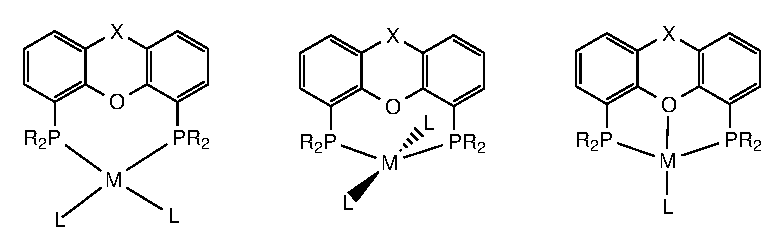
\includegraphics{../Figures/Bondingmodes.eps}
%\caption[Different bonding modes of xantphos ligands]{Different bonding modes of xantphos ligands}
%\vspace{0.2cm}
%\label{Bondingmodes}
%\end{center}
%\end{figure}
%\vspace{0.2cm}
%%
%%\chapter{Introduction}
%%\label{ch:introduction}
%%
%%It is now widely accepted that climate change is occurring at an unprecedented rate.\cite{Oreskes2004}  The concentration of greenhouse gases such as carbon dioxide, methane and nitrous oxide in the atmosphere has been increasing since the industrial revolution (Figure~\ref{Greenhousegases})\cite{Jacobs1999}.  In addition, new greenhouse gases such as \glspl{CFC} are also accumulating in the atmosphere.  \cite{Jacobs1999}  Energy from the sun is absorbed by the surface of the earth and then radiated out into the atmosphere at wavelengths between 5 and 50 \SI{}{\micro\metre}.  Much of this energy is absorbed by atmospheric gases such as ozone and water vapour, however there is a small ``atmospheric window'' between 8 and 13 \SI{}{\micro\metre} where energy can escape into the solar system.  Greenhouse gases in the atmosphere absorb energy in this atmospheric window and rather than letting the energy escape into the solar system, it is radiated back towards earth.\cite{Hardy2003}  As such, the increased atmospheric greenhouse gas concentrations lead to increases in global temperature.\cite{Jacobs1999}
%%
%%Carbon dioxide absorbs strongly above 10 \SI{}{\micro\metre} making it a potent greenhouse gas.\cite{Goody1951}  Prior to the industrial revolution, the amount of carbon dioxide released into the atmosphere was balanced by the amount taken up by natural sinks such as the oceans and the biosphere.  However, the burning of fossil fuels has increased the amount of carbon dioxide released into the atmosphere.  As the carbon in the fossil fuels has been effectively removed from the natural carbon cycle for millennia, the natural sinks for carbon dioxide (biosphere and oceans) have been unable to cope with the increase in concentration resulting in accumulation within the atmosphere.\cite{Jacobs1999}
%%
%%\begin{figure}[h]  
%%\centering
%%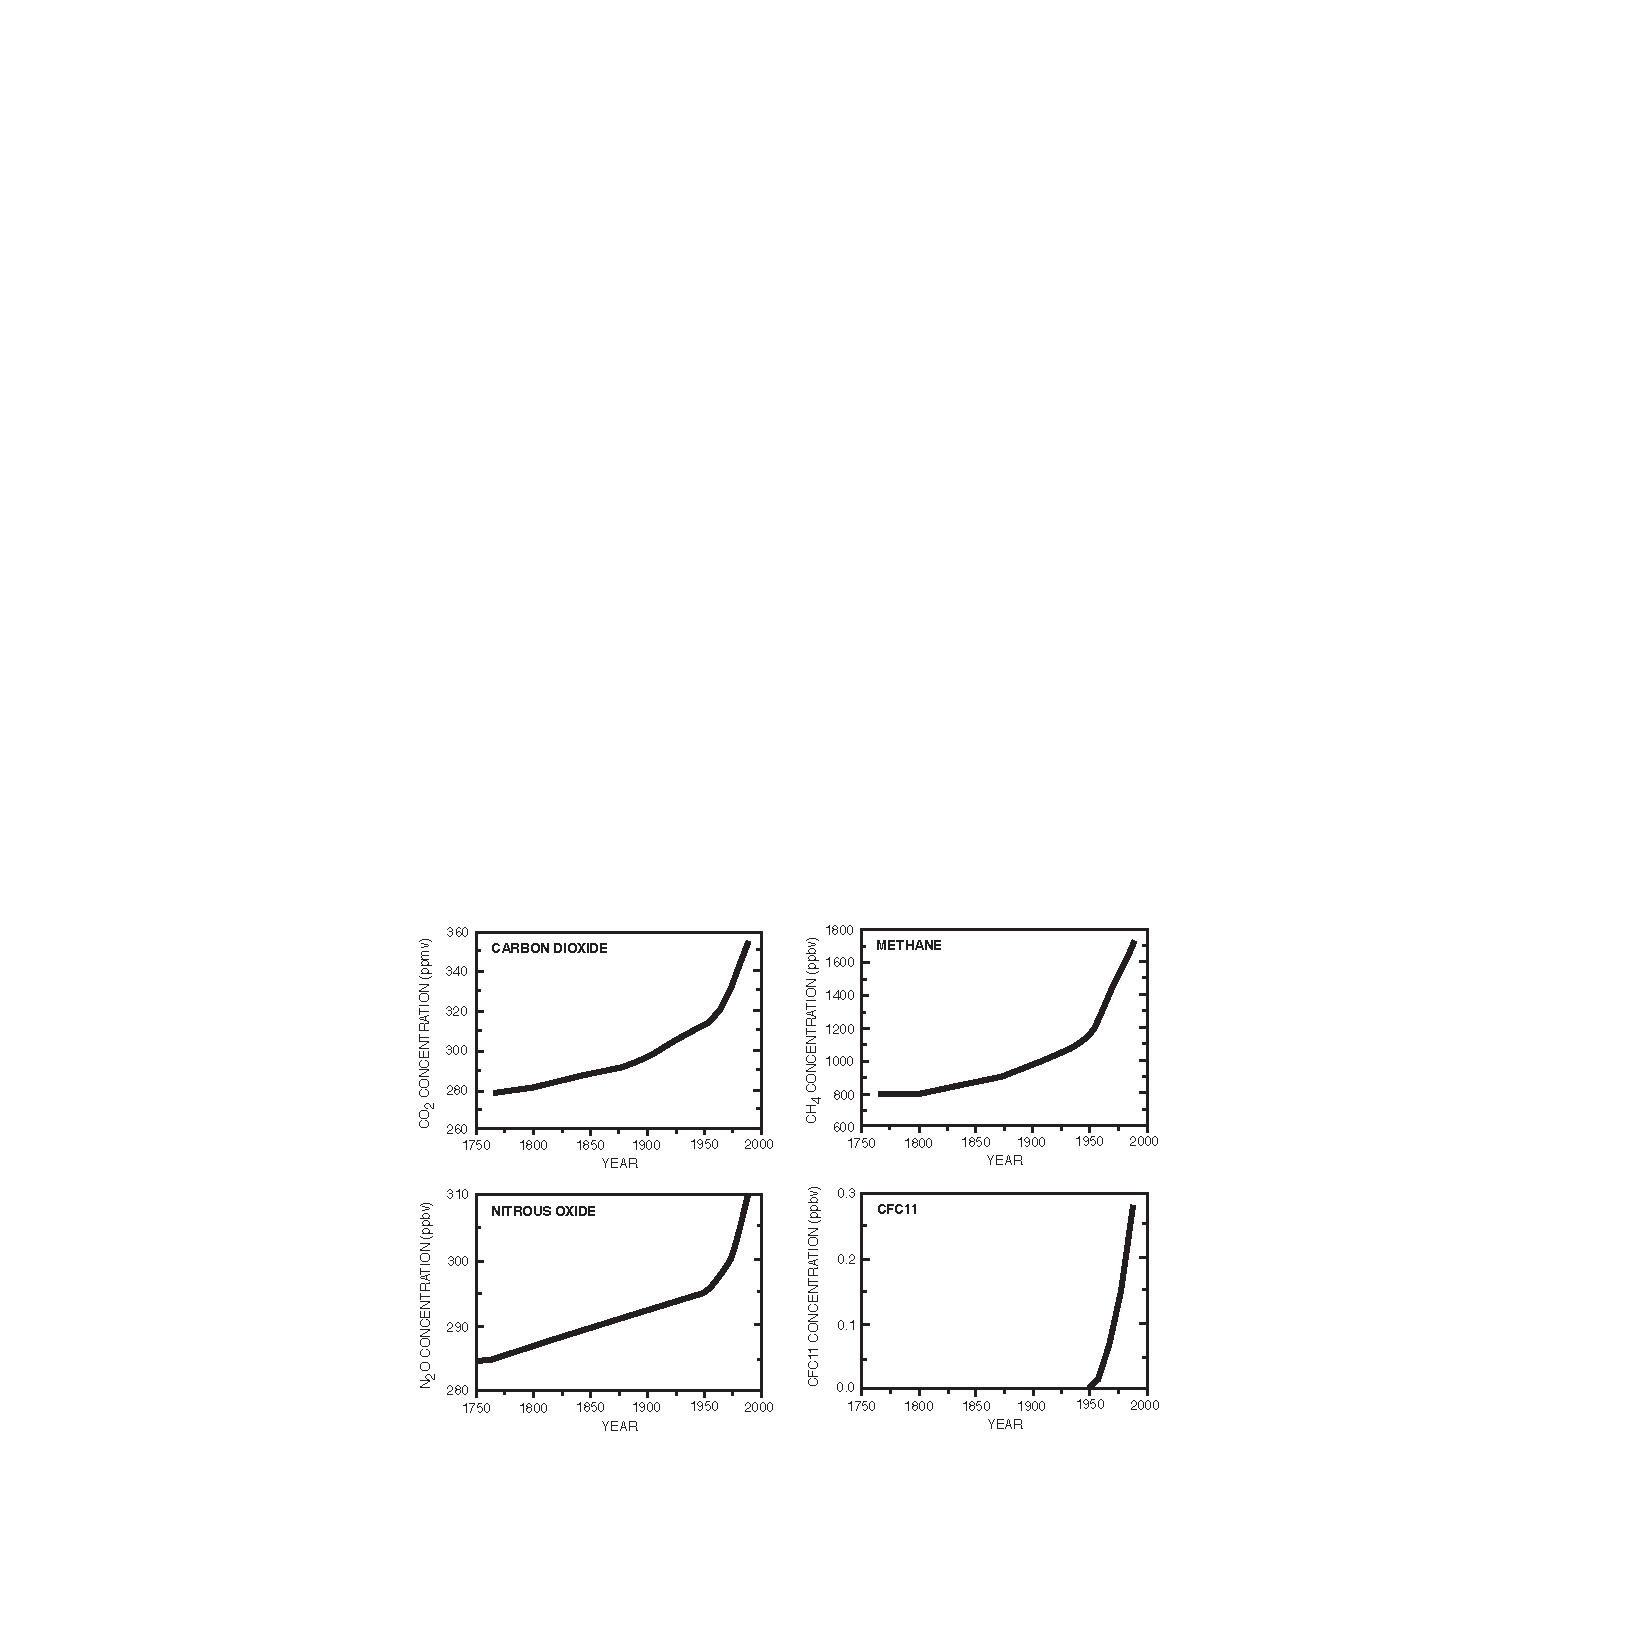
\includegraphics[width = \textwidth]{../Figures/Greenhousegases.pdf}
%%\caption[Concentration of greenhouse gases]{Rise in concentration of greenhouse gases since the 18th century.  Reproduced from \emph{Introduction to Atmospheric Chemistry} p. 113.\cite{Jacobs1999}}
%%\label{Greenhousegases}
%%\end{figure}
%%
%%Fossil fuels are also a prominent source of chemical feedstocks.\cite{Shilov1997}  The alkanes can be converted into alkenes and alkynes \emph{via} hydrothermal cracking and these can be oxidised or otherwise converted to form useful chemical starting materials.  However, the hydrothermal cracking is highly inefficient requiring high temperatures and producing a large range of undesirable by-products.\cite{Shilov1997}  The potential environmental damage from using fossil fuels, together with the mounting costs associated with their extraction, means alternative chemical feedstocks are desirable both environmentally and economically.\cite{Poliakoff2002, Crabtree2011b}
%%
%%Biogas is a mixture of gases containing primarily methane and carbon dioxide with small amounts of hydrogen sulfide, ammonia and other impurities.\cite{Abatzoglou2009}  Generated by the anaerobic digestion of wet organic waste, biogas is considered carbon neutral as the carbon in the organic matter, which is converted to the biogas, is already within the carbon cycle.\cite{Amon2007}  New Zealand has a number of plants to capture the biogas produced from landfill, sewage, farm and food waste.\fixme{cite(Biogas)}  Typically the biogas collected is used for on-site electricity production or co-generation of electricity and methane.
%%
%%%\begin{table}
%%%\caption[Biogas generation sites in New Zealand]{Biogas generation sites in New Zealand}
%%%\label{Biogas}
%%    %\begin{tabular}{l p{4cm} l l}
%%    %\hline
%%%Project name & Feedstock & Application & Year Commissioned\\ \hline
%%%PNCC digester upgrade & Co-digestion & Co-generation & 2008/10\\ 
%%%HCC Digester upgrade (Hamilton) & Co-digestion & Co-generation & projected\\ 
%%%Beef feedlot manure (Waikato)	& Feedlot waste & Study & 2008\\ 
%%%Piggery feedlot manure (Waikato)& Feedlot waste & Study & 2008\\
%%%Chicken Waste (Waikato)	& Industrial & Study / Research & 2008\\ 
%%%Tirau Dairy (Tirau) & Industrial waste & Boilers & 1990\\
%%%Southern Landfill, Happy Valley & Landfill & Power generation & 2008\\
%%%Silverstream (Lower Hutt)	& Landfill & Power generation & 1994\\
%%%Greenmount & Landfill & Power generation & 1992\\ 
%%%Rosedale & Landfill & Power generation & 1994\\
%%%Horotiu Landfill & Landfill & Power generation & 2004\\
%%%Spicer Landfill (Porirua/Wellington) & Landfill & Flaring & 2009 \\ 
%%%Burwood Landfill & Landfill & Co-generation & 2007\\
%%%Tirohia Landfill	& Landfill & Power generation & 2008\\
%%%Hampton Downs Landfill & Landfill & Power generation &2009\\
%%%Landcorp (Waimakariri/Rangiora) & Manure biosolids & Co-generation & 2007/08\\
%%%Kiwifruit Waste (Tauranga) & Rural waste & Study & 2008 \\
%%%Piggery Waste (Canterbury) & Rural waste & Study	& 2008\\ 
%%%Piggery Waste (Waikato)	& Rural waste & Research & 2008\\ 
%%%Piggery Waste (Canterbury) & Rural waste & Study & 2009\\ 
%%%Mangere WWTP I(Auckland) & Sewage & Co-generation	& 2004\\ 
%%%Hamilton WWTP (Hamilton ) & Sewage & Co-generation	& 2005\\
%%%Bromley WWTP & Sewage & Co-generation & 1996\\ 
%%%Tauranga WWTP & Sewage & Co-generation & 1996\\ 
%%%CCC digester upgrade (Christchurch) & Thermophilic / biosolids & Co-generation & projected\\
%%%GI digester (Dunedin) & Thermophilic / biosolids & Boilers & 2001\\
%%    %\hline
%%    %\end{tabular} \end{table}
%%
%%Biogas also has the potential to act as a chemical feedstock for industrial processes that typically use components extracted from crude oil.\cite{Poliakoff2002}  However, there are several issues associated with the use of biogas as a chemical feedstock.  Biogas is often produced at remote sites and as it mostly contains methane, it cannot be transported economically,\cite{Crabtree2001} hence on-site conversion of the methane into a readily transportable liquid such as methanol would reduce the transportation costs considerably.  However methane, like other alkanes, is unreactive towards most chemical transformations.  Although methane can be oxidised, the low reactivity means that severe conditions or highly active reagents are required.  The methanol that is produced is more easily oxidised than methane so over-oxidation to the undesirable carbon dioxide occurs readily. \cite{Crabtree2001}  
%%
%%One of the most commonly used processes to form methanol from methane is the syngas process.  This first converts the methane to carbon monoxide, then reduces it to methanol.  The formation of synthesis gas (Equation \ref{syngasequation}) is carried out over a heterogeneous nickel catalyst and requires pressures of 40 atm and high temperatures of 850 \degrees C.  This is followed by reaction over a mixture of copper, zinc oxide and alumina at 50 - 100 atm and 250 \degrees C (Equation \ref{syngasequation2}). The process is inefficient as the methane is over-oxidised before being reduced to methanol\cite{Crabtree2001} and although the production of synthesis gas yields three moles of hydrogen, only two of these are used in the production of methanol.  The addition of \ce{CO2} to the system allows for reaction of the excess hydrogen to produce methanol and water (Equation \ref{syngasequation3}).
%%
%%\vspace{-1cm}
%%\begin{align}
%%\ce{CH4 + H2O} & \longrightarrow \ce{CO + 3H2} \label{syngasequation} \\[0.5cm]
%%\ce{CO + 2H2} & \longrightarrow \ce{CH3OH} \label{syngasequation2} \\[0.5cm]
%%\ce{CO2 + 3H2} & \longrightarrow \ce{CH3OH + H2O} \label{syngasequation3}
%%\end{align}
%%\vspace{-2cm}
%%%Green chemistry aspect\\
%%%CO2 harming the atmosphere\\
%%%Carbon cycle\\
%%%QC comic http://questionablecontent.net/view.php?comic=1939\\
%%
%%\section{C-H activation}
%%
%%Carbon-hydrogen bonds are among the least reactive bonds as evidenced by their presence in all organic molecules.\cite{Shilov1997}  Indeed the old name for alkanes ``paraffins'' is derived from the Latin \emph{parum affinis} meaning without affinity.  Alkanes have also been referred to as the ``noble gases of organic chemistry.''\cite{Shilov1997}  The carbon-hydrogen bond is considered to be a very strong bond with a bond dissociation enthalpy of 438~kJmol$^{-1}$ for methane.\fixme{cite
%%(SI2002)}  This compares to an average carbon-oxygen bond of 358~kJmol$^{-1}$, and a carbon-carbon single bond of 346~kJmol$^{-1}$.\fixme{cite(SI2002)}  In addition, alkanes have very high ionisation potentials and pK\sub{a} values, and low proton affinities.\cite{Shilov2000}  Alkenes typically have stronger C-H bonds than alkanes, for example ethene and ethyne have bond dissociation enthalpies of 444 and 502 kJmol$^{-1}$ respectively, compared to 410 kJmol$^{-1}$ for ethane.\cite{Shilov1997}  However, the reduced steric hindrance in alkenes leads to greater kinetic reactivity, and stronger aryl-metal bonds result in a thermodynamic driving force for the C-H activation to occur.\cite{Crabtree2001}
%%
%%%bond lengths 1.08 C-H, 1.43 C-O, 1.54 C-C
%%
%%%Ethene, ethyne and benzene all have stronger C-H bonds of 444, 502 and 456 .\cite{Shilov1997}  As such, a carbon-hydrogen bond in an alkane is unlikely to react without strong reagents or severe conditions.\cite{Crabtree2001}
%%
%%C-H activation refers to the increased reactivity of carbon hydrogen bonds that occurs as a result of interaction with another reagent.\cite{Crabtree2001}  Functionalisation involves the replacement of the C-H bond with another functional group (X) to form a C-X bond.  This reaction may occur in a number of different ways depending on the reactivity of the metal complex.\cite{Shilov2000}  Activation is typically easier than functionalisation as the metal alkyl and hydride often recombine \emph{via} reductive elimination during attempts to functionalise.\cite{Crabtree2001}  
%%%However, the functionalisation is crucial for the conversion of methane to a useful feedstock.
%%
%%%The functionalisation step may be viewed as a organic reaction occuring on a metal support which is important for the activation of the bond.\fixme{reword this?}  
%%
%%%This is essentially an organic reaction following activation.\cite{Crabtree2001}  
%%
%%There are three main processes by which C-H activation can occur.\cite{Shilov2000}  The first is the organometallic activation which involves the formation of a metal-carbon bond.  This may involve cleavage of the bond through either oxidative addition (Equation \ref{Oxidativeequation}) or electrophilic substitution (Equation \ref{Electrophilicequation})  In the second type the alkane C-H bond interacts with a ligand on the metal rather than the metal itself (Equation \ref{Oxidationequation}).  The third type involves the generation of a reactive species by the metal complex, which then attacks the C-H bond (Equation \ref{Radicalequation}).  Systems where organometallic activation occurs will be the focus of this proposal.
%%
%%\vspace{-1cm}
%%\begin{align}
%%\ce{RH + M}^{n+}	& \longrightarrow	\ce{[R-M-H]}^{n+2} \label{Oxidativeequation} \\[0.5cm]
%%\ce{RH + M}^{n+}	& \longrightarrow	\ce{R-M}^{(n+2)+} + \ce{H+} \label{Electrophilicequation} \\[0.5cm]
%%\ce{RH + O=M}^{n+} 	& \longrightarrow	\ce{R\dot} + \ce{HO-M}^{(n-1)+} \label{Oxidationequation} \\[0.5cm]
%%\ce{H2O2 + Fe}^{2+}	 & \longrightarrow	\ce{HO\dot{} + HO- + Fe}^{3+} \label{Radicalequation} \\
%%\ce{HO\dot} + \ce{RH} & \longrightarrow	\ce{H2O + R\dot} \notag \\[0.5cm]
%%\ce{CH4 + 2O2} & \longrightarrow \ce{CO2 + 2H2O} \label{Combustion}
%%\end{align}
%%
%%%\fixme{similarities between C-H and H-H activation}
%%
%%Alkanes can react at elevated temperature with oxygen in the atmosphere to form the thermodynamically stable products water and carbon dioxide (Equation \ref{Combustion}).  However, alkanes are inert in air at room temperature in the absence of a catalyst.\cite{Shilov1997}  Alkanes can be converted into other hydrocarbons by heating.  This forms radical species which can combine to form longer or shorter chain alkanes, alkenes and alkynes.\cite{Sironi1990}  For example, methane may be converted into ethane, ethene and ethyne by heating at temperatures in excess of 900 \degrees C.\cite{Shilov1997}  Alkanes can also be protonated by superacids, leading to elimination of hydrogen gas, giving an overall hydride abstraction reaction.  However, the elimination occurs selectively with the most basic hydride and the superacids used will attack a number of functional groups.\cite{Crabtree2004}
%%
%%%\vspace{-0.8 cm}
%%%\begin{equation}
%%
%%%\label{Combustion}
%%%\end{equation}
%%
%%The presence of other functional groups on the molecule can result in activation of a C-H bond.  A common example of this is protons $\alpha$ to a carbonyl group that are easily removed in the presence of a base.  This forms the basis for a number of widely utilised organic reactions such as the aldol condensation reaction (Scheme~\ref{Aldolcondensation})\cite{Saito2004}.  However in alkanes, no functional groups are present to activate the bond so it is necessary to activate the bond using an external source such as an enzyme or coordination complex.\cite{Crabtree2001}
%%
%%\begin{scheme}[h]  
%%  \centering
%%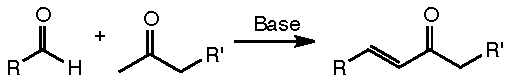
\includegraphics[]{../Schemes/Aldolcondensation.pdf}
%% \caption[Aldol condensation reaction]{Aldol condensation reaction}
%% \label{Aldolcondensation}
%%\end{scheme}
%%
%%%104 kcal mol-1 = ~435 kJmol-1
%%
%%Complex organic molecules are synthetic targets as a result of their potential use as pharmaceuticals.  Currently the synthesis of these target molecules relies on the modification of existing functional groups.  The regio- and stereo-selective activation and functionalisation of C-H bonds within complex organic molecules would result in a major paradigm shift in organic synthesis.\cite{Davies2008}
%%
%%\subsection{Biological systems}
%%
%%As previously discussed, the oxidation of methane to methanol without over-oxidation to carbon dioxide is desirable in order to make use of biogas as a chemical feedstock.\cite{Crabtree2001}  Like many other desirable chemical transformations, enzymes exist that are capable of performing the reaction.  Methane monooxygenase and cytochrome P450 catalyse the oxidation of alkanes to alcohols (Equation \ref{Methanemonooxygenaseequation}).\cite{Crabtree1995}  Although methane monooxygenase is specfic for methane, cytochrome P450 enzymes will catalyse the oxidation of a range of alkanes.\cite{Lipscomb1994, Crabtree2001}
%%
%%\vspace{-0.8 cm}
%%\begin{equation}
%%\ce{NADPH + O2 + RH + H+} \longrightarrow \ce{NADP+ + H2O + ROH}
%%\label{Methanemonooxygenaseequation}
%%\end{equation}
%%
%%Methane monooxygenase is found in bacteria that exist at the interface of aerobic and anaerobic environments found in lakes, oceans and soils.\cite{Lipscomb1994}  These bacteria are described as methanotrophic, they utilise methane as their source of carbon and energy.\cite{Haber1983}  Methane monooxygenase consists of three proteins; component B, reductase and hydroxylase.\cite{Lipscomb1994}  The hydroxylase protein contains a dinuclear iron centre that activates oxygen to form an oxo-bridged system.  This reacts with methane to give methanol and a hydroxo-bridged diiron centre.\cite{Merkx2001}  However, despite numerous studies,\cite{Lipscomb1994, Merkx2001, Tinberg2011} the mechanism of methane monooxygenase has proved elusive with a number of different mechanisms proposed (Scheme \ref{Methanemonooxygenasemechanism}).
%%
%%%The hydroxylase protein contains a hydroxo-bridged dinuclear iron that forms that active catalytic site.  Both iron atoms are reduced to Fe(II) and then react with \ce{O2} The O-O bond is cleaved to give water and a Fe(IV)Fe(IV)=O species which can abstract a hydrogen from methane.  This gives an OH radical and a \ce{CH3} radical which recombine to form methanol.\fixme{SCHEME}
%%
%%%\begin{figure}[h]
%%%\centering
%%%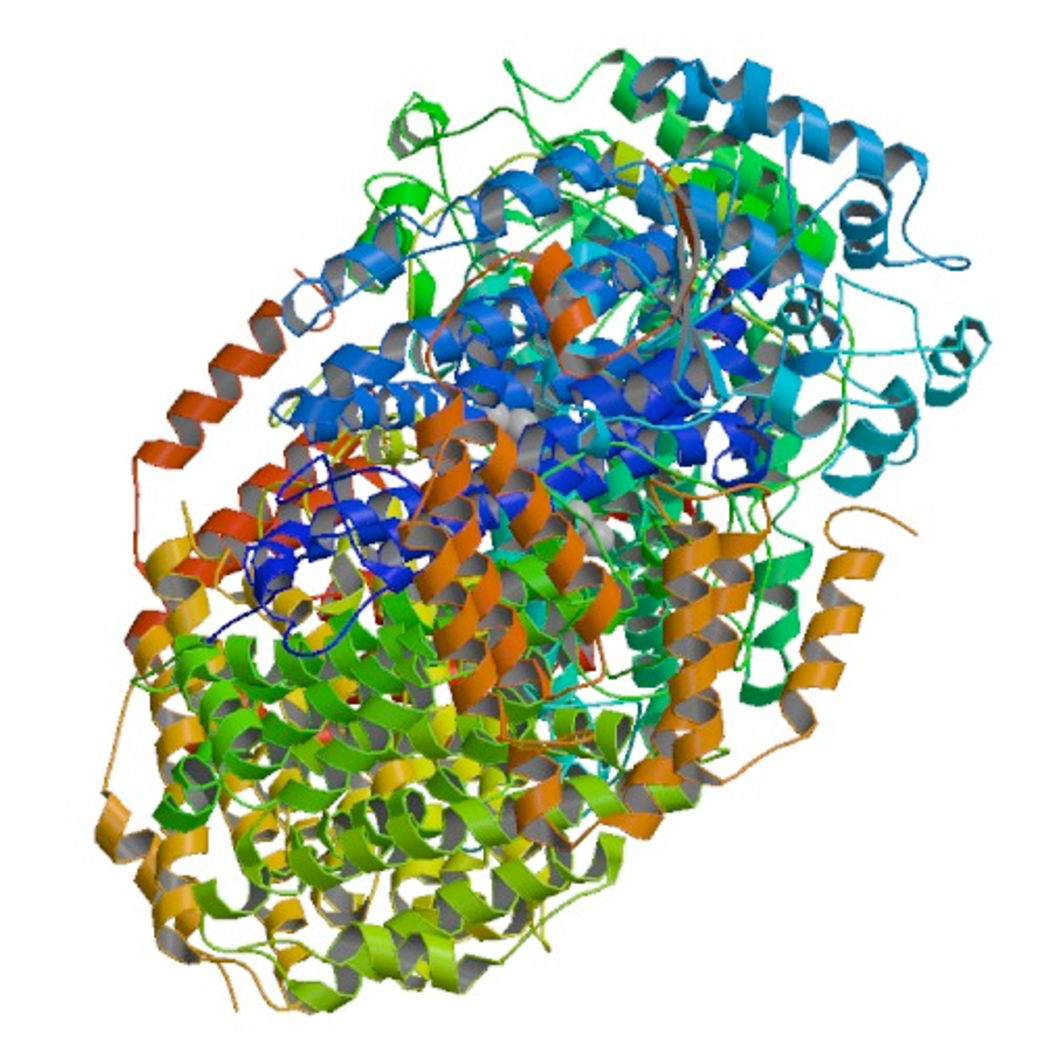
\includegraphics[height = 5cm]{../Figures/Methanemonooxygenase.pdf}
%%%\caption[X-ray crystal structure of methane monooxygenase]{X-ray crystal structure of methane monooxygenase reproduced from \fixme{reference from protein databank}}
%%%\label{Methanemonooxygenase}
%%%\end{figure}
%%
%%\begin{scheme}[h]
%%\centering
%%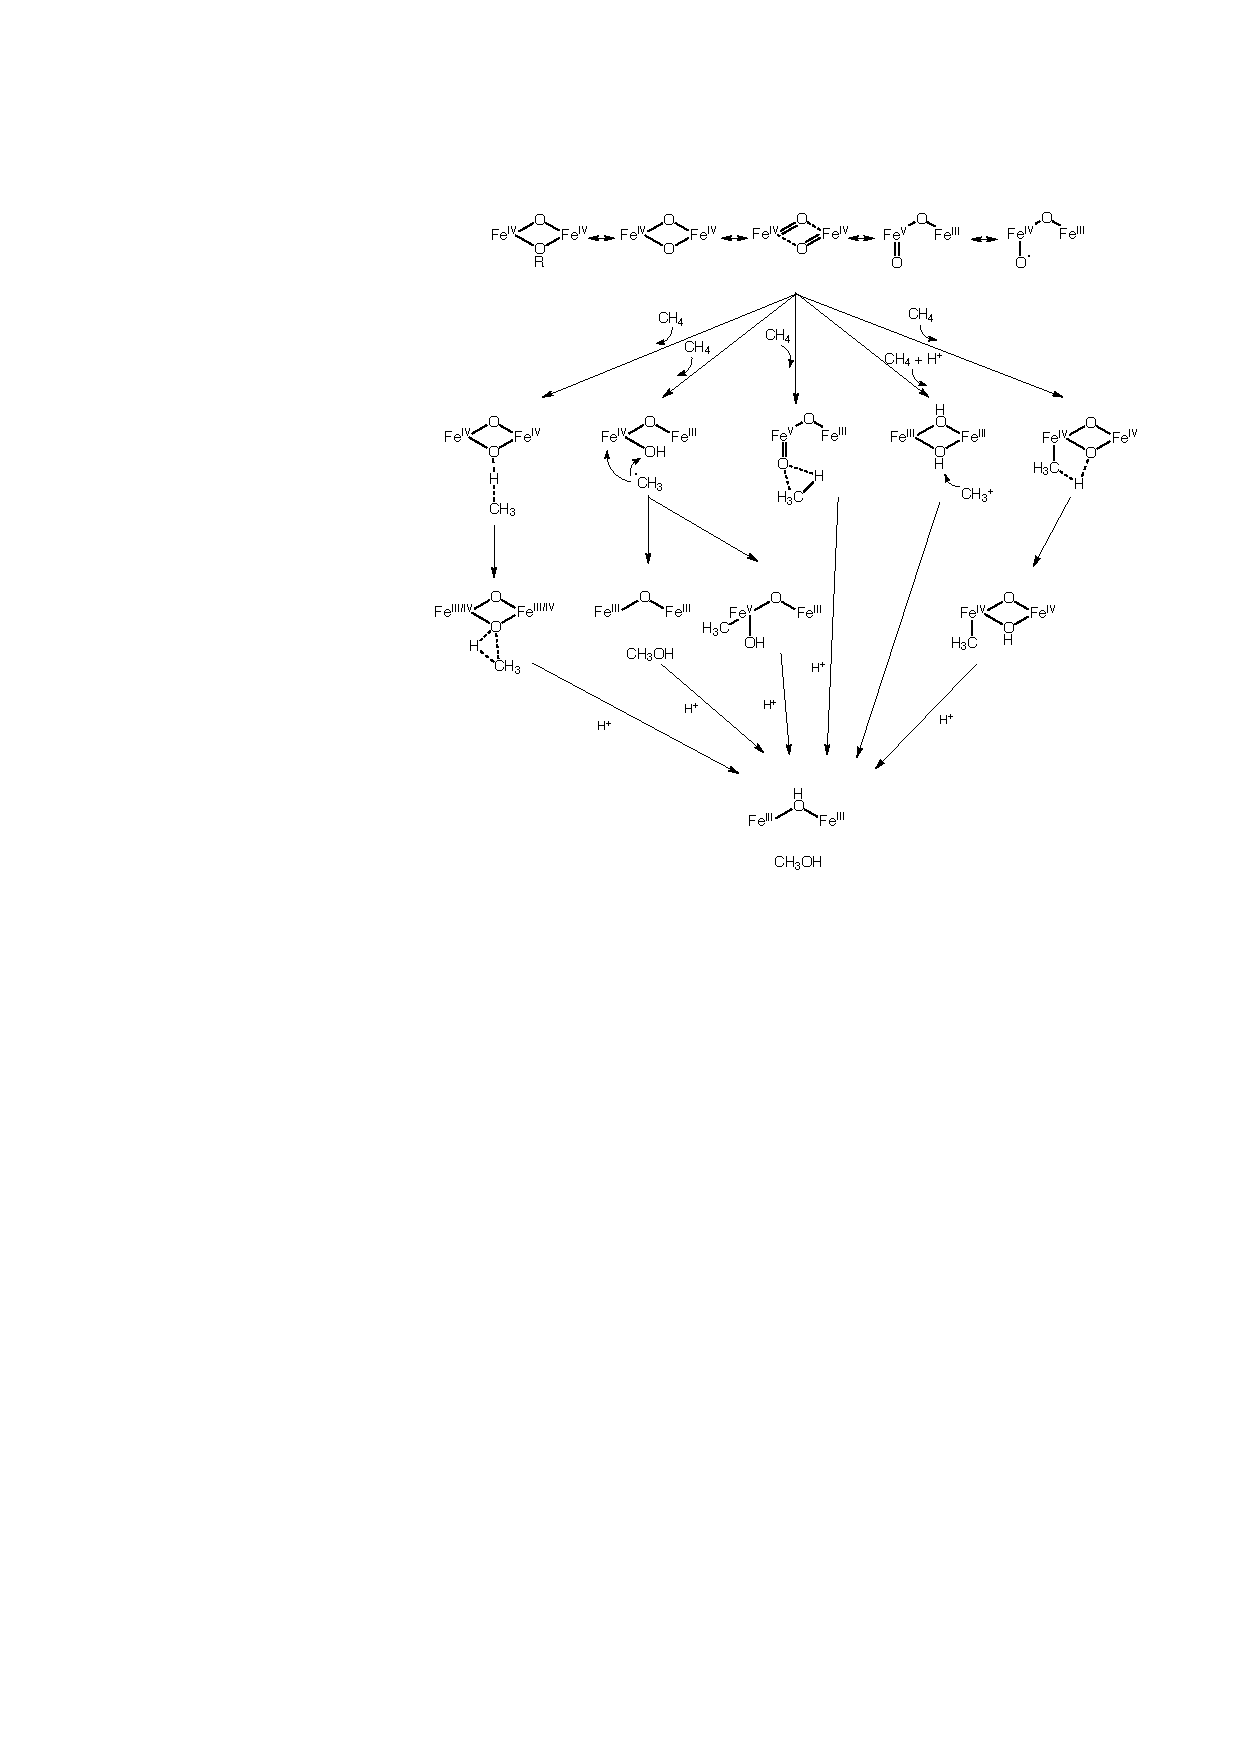
\includegraphics[width = 0.95\textwidth]{../Schemes/Methanemonooxygenasemechanism.pdf}
%%\caption[Proposed mechanisms for the hydroxylation of methane]{Proposed mechanisms for the hydroxylation of methane reproduced from Lippard et al.\cite{Merkx2001}}
%%\label{Methanemonooxygenasemechanism}
%%\end{scheme}
%%
%%Cytochrome P450 enzymes are found in a most classes of organisms including bacteria, fungi, plants, insects and mammals.\cite{Montellano2010}  The consistent feature across all P450 enzymes is the presence of a heme group with a coordinated thiolate ion at the active site of the molecule.\cite{Montellano2010}  The first step in metabolism of pharmaceuticals in the body, phase 1, typically involves oxidation, reduction and hydrolysis reactions.  P450 enzymes are responsible for the phase 1 metabolism of around 75\% of known pharmaceuticals.\cite{Rittle2010}  Although the enzymes perform a number of roles, one of the most interesting is the hydroxylation of C-H bonds.\cite{Rittle2010}
%%
%%The overall catalytic cycle for the hydroxylation of an alkane by a P450 enzyme reported by de Montellano\cite{Montellano2010} is given in Scheme \ref{P450catalyticcycle}.  In the resting state (A) the Fe(III) is bound to a thiolate and the \emph{trans} ligand is typically a water molecule though some P450's do not have a \emph{trans} ligand.  The water is displaced upon binding of an RH group.  Binding of the RH allows electron transfer to occur, reducing the Fe(III) to Fe(II) (C).  Oxygen binds to the Fe(II) resulting in the superoxide complex D.  This undergoes electron transfer and protonation to form the hydroperoxo complex E.  This complex is protonated and undergoes loss of \ce{H2O} to form the porphyrin radical cation F.  F can then react with the substrate to give the alcohol product.  Following product release and rebinding of water the resting state is restored.
%%
%%%\begin{figure}[h]
%%%\centering
%%%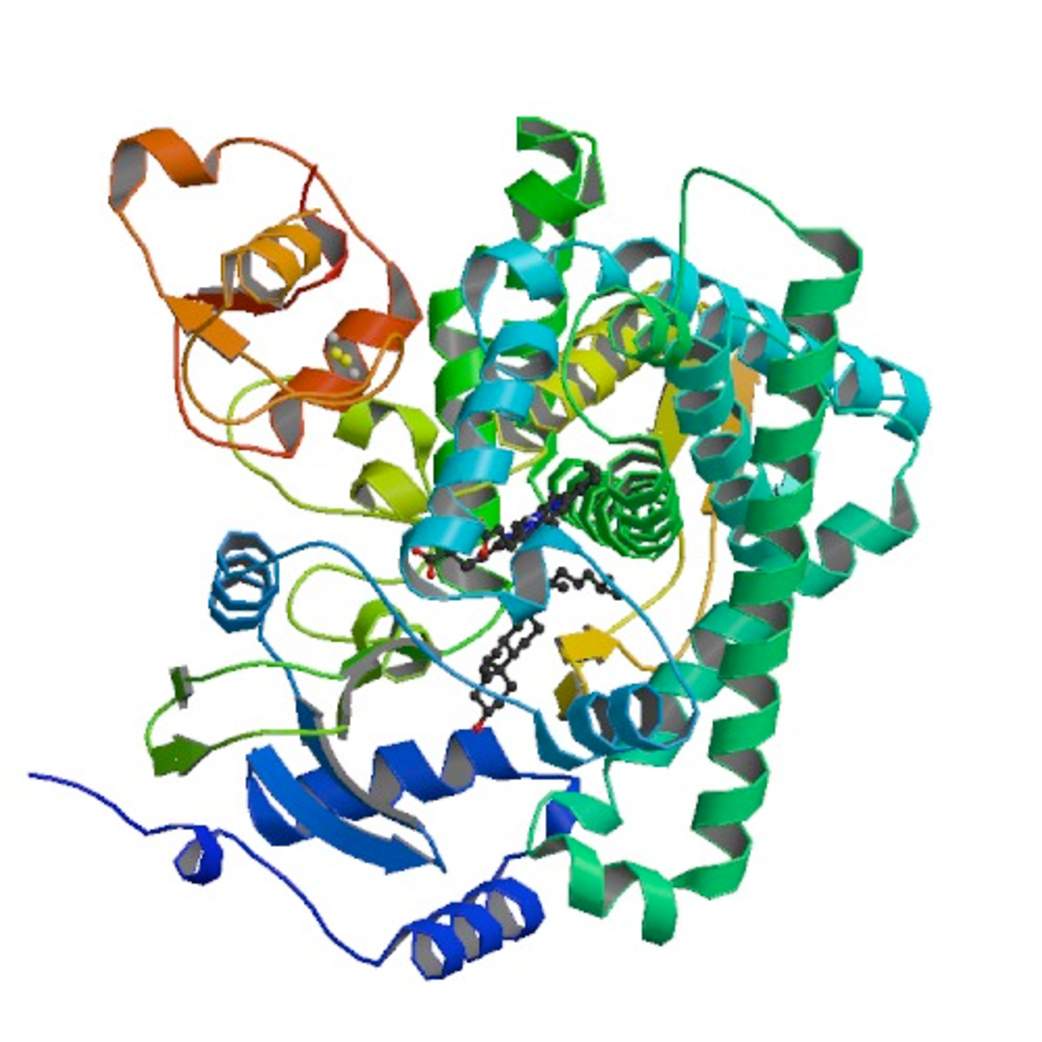
\includegraphics[height = 5cm]{../Figures/P450.pdf}
%%%\caption[X-ray crystal structure of P450]{X-ray crystal structure of P450 reproduced from \fixme{reference from protein databank}}
%%%\label{P450}
%%%\end{figure}
%%
%%\begin{scheme}[ht]
%%\centering
%%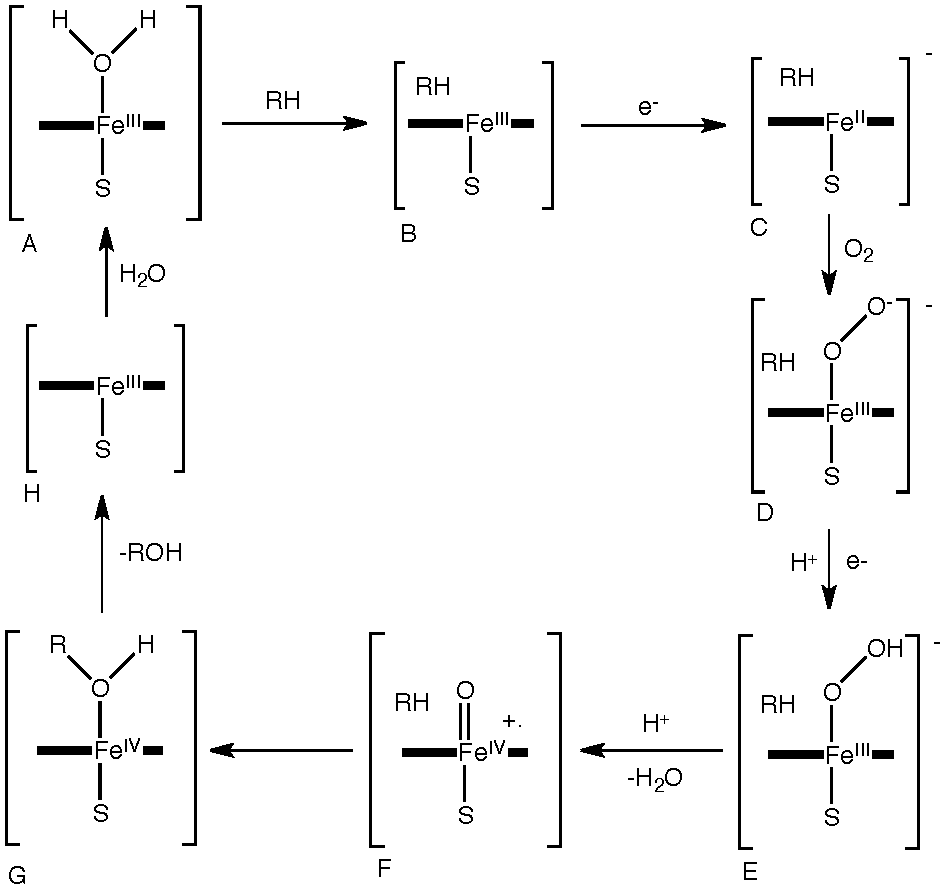
\includegraphics[width = 0.75\textwidth]{../Schemes/P450catalyticcycle.pdf}
%%\caption[Proposed catalytic cycle for hydroxylation by P450]{Proposed catalytic cycle for hydroxylation by P450 reported by de Montellano\cite{Montellano2010}}
%%\label{P450catalyticcycle}
%%\end{scheme}
%%
%%\subsection{Organometallic systems}
%%
%%There are a number of different types of bonds that can form in organometallic systems (Figure \ref{Bondingmodesintro}).  The most common is the donation of a ligand lone pair of electrons to a vacant orbital on the metal (a).  This is typically observed for ligands such as \ce{PR3,~CH3^-~and~H2O} among many others.  Donation of a $\pi$-bonding pair of electrons to the metal (b) is also common, typically among the alkene complexes such as those with ethene.  There are a number of rarer bonding forms including the donation of a $\sigma$-bonding pair of electrons (c) and the alkyl agostic interaction (d).\cite{Bernskoetter2009}  In addition, the metal can donate electron density from filled d orbitals into the LUMO of the ligand (either the $\sigma$* or $\pi$* orbital).\cite{Chatt1955}
%%
%%\begin{figure}[ht]
%%\centering
%%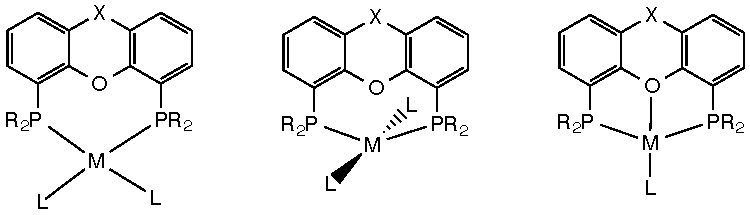
\includegraphics[width = 0.5\textwidth]{../Figures/Bondingmodes.pdf}
%%\caption[Bonding in organometallic complexes]{Bonding in organometallic complexes}
%%\label{Bondingmodesintro}
%%\end{figure}
%%
%%Alkanes are weak $\sigma$-bases and $\pi$-acids.  As such they are very poor ligands for transition metals.\cite{Crabtree1993}  Typically alkanes form $\sigma$-complexes with metals that can $\pi$-backbond.  For successful complexation a low valent metal and the absence of competitive decomposition pathways are required.\cite{Crabtree2001}  Enhanced bonding of alkanes occurs with metals capable of forming enhanced $\pi$-backbonding into the $\sigma$* C-H orbital, similar to that found for molecular hydrogen complexes.\cite{Kubas1988}
%%
%%The activation of C-H bonds is thought occur \emph{via} a stepwise process involving the coordination of the alkane to the metal to form a $\sigma$-complex, followed by the oxidative cleavage of the C-H bond forming metal-alkyl and metal-hydride bonds.\cite{Labinger2002}  The intermediate  $\sigma$-complexes are highly unstable and until recently their existence had only been inferred by isotope scrambling and the inverse kinetic isotope effect in reductive elimination reactions of alkyl hydrides.\cite{Bernskoetter2009, Labinger2002}  In 2009 Brookhart reported the characterisation of a relatively long-lived rhodium(I) $\sigma$-methane complex.\cite{Bernskoetter2009}  The complex was formed by the protonation of a rhodium methyl complex (Scheme \ref{Sigmamethane}).  At -87~\degrees C the methane is displaced by solvent (\ce{CDCl2F}) with a half-life of 83 minutes.
%%
%%\begin{scheme}[ht]
%%\centering
%%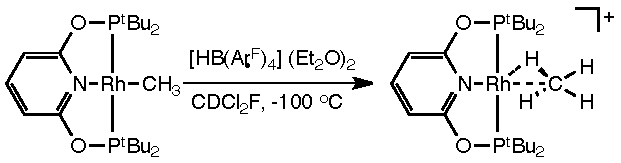
\includegraphics[]{../Schemes/Sigmamethane.pdf}
%%\caption[Formation of a $\sigma$-methane complex]{Formation of a $\sigma$-methane complex.  Ar\ce{^{F}} = \emph{m}-di(trifluoromethyl)phenyl}
%%\label{Sigmamethane}
%%\end{scheme}
%%
%%%$\sigma$-Complexes of methane have been proposed 
%%%The first example of C-H activation was reported by Dimroth in 1902\cite{Dimroth1902}  Reaction of phenol with a solution of mercury acetate on a steam bath replaced the \emph{ortho} and \emph{para}-protons with a mercury acetate group.  \fixme{more info etc}
%%
%%C-H activation has developed significantly since the first example of C-H activation by an organometallic complex was reported by Chatt in 1962. \cite{Chatt1962}  Reduction of metal halides by sodium napthalene in the presence of an excess of \gls{dmpe} produced V, Cr, Mo and W complexes of the form \ce{[M(}\gls{dmpe}\ce{)_3]},  and Fe and Co complexes of the form \ce{[M(}\gls{dmpe}\ce{)_2]}.  However, the \ce{[Ru(}\gls{dmpe}\ce{)_2]} analogue gave a hydride complex ``by taking hydrogen from the napthalene.''\cite{Chatt1962}  
%%
%%Further analysis of the ruthenium system was carried out and published in 1965.\cite{Chatt1965} Reaction of \emph{cis}- or \emph{trans}-\ce{[RuCl2(}\gls{dmpe}\ce{)_2]} with benzene, naphthalene, anthracene and phenylanthracene formed the \emph{cis}-\ce{[RuH(aryl)(}\gls{dmpe}\ce{)_2]} (aryl = phenyl, naphthyl, anthryl and phenanthryl) complexes \emph{via} oxidative addition.\cite{Chatt1965}  The activation is reversible, as reactions of the complexes with hydrochloric acid yielded hydrogen gas, the aromatic starting material and \emph{cis}-\ce{[RuCl2(}\gls{dmpe}\ce{)_2]} (Equation \ref{ChattCH}).  The C-H activation to form the complexes was selective for example, in the reaction with naphthalene the activation occurred exclusively at the 2-position.
%%
%%\vspace{-0.6 cm}
%%\begin{equation}
%%\ce{[RuH(C10H7)(dmpe)2] + 2HCl} \longrightarrow \ce{[RuCl2(dmpe)2] + H2 + C10H8}
%%\label{ChattCH}
%%\end{equation}
%%
%%The naphthyl hydride complex formed by treatment of \ce{[Ru(}\gls{dmpe}\ce{)_2]} with naphthalene thermally decomposed giving a complex with properties consistent with \ce{[Ru(}\gls{dmpe}\ce{)_2]} (Scheme \ref{Chattdmpescheme}).\cite{Chatt1965}  However, infrared spectroscopy showed a signal for a Ru-H at 1791 \percm,  leading to the proposed structure of \ce{[RuH(CH2PMeCH2CH2PMe2)(}\gls{dmpe})], formed by activation of a C-H bond from the \gls{dmpe} ligand.\cite{Chatt1965}  X-ray crystallography later allowed the reformulation of the structure to the analogous dimer.\cite{Crabtree2004}  However, this species remains the first example of cyclometallation of an sp$^3$ C-H bond.
%%
%%\begin{scheme}[ht]
%%\centering
%%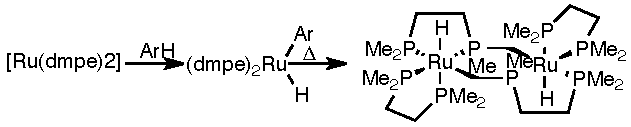
\includegraphics[]{../Schemes/Chattdmpescheme.pdf}
%%\caption[C-H activation reactions reported by Chatt and Davidson]{C-H activation reactions reported by Chatt and Davidson\cite{Chatt1965}}
%%\label{Chattdmpescheme}
%%\end{scheme}
%%
%%The exchange of hydrogen with deuterium in polyalkyl benzenes, polycyclic aromatic hydrocarbons and heterocycles can be catalysed by homogeneous platinum (II) species.\cite{Hodges1968, Hodges1969, Hodges1969b}  Using deutero-acetic acid as a solution in \ce{D2O}, together with DCl or anhydrous tin(IV) chloride to prevent the formation of platinum metal, H/D exchange on the substrate was observed when exposed to \ce{Na2PtCl4} or \ce{K2PtCl4}.\cite{Hodges1968, Hodges1969}  Although the rate of exchange was faster for unhindered aromatic protons, H/D exchange was also observed for alkyl protons.\cite{Hodges1969b}  The rate was fastest for \hbox{\emph{p}-xylene}, \gls{mesitylene}, \emph{m}-xylene and toluene, however exchange of alkyl protons was also observed in \emph{o}-xylene, \gls{hemimellitene} and \gls{durene}.\cite{Hodges1969b}
%%
%%This activation of alkyl protons inspired Shilov to investigate the C-H activation of alkanes by platinum.  The system carries out oxidation of alkanes such as methane \emph{via} electrophilic activation (Scheme \ref{Shilovcatalyticcycle}).\cite{Labinger2002, Crabtree2001}  The first step involves displacement of a chloride ligand on the platinum by a $\sigma$-methyl followed by oxidative addition and loss  of H$^+$ \emph{via} loss of HCl.  The Pt(II) is then  oxidised to Pt(IV) \emph{via} electron transfer to the \ce{PtCl6}$^{2-}$.  Finally, the complexed methyl undergoes nucleophilic attack from water displacing the \emph{trans} chloride ion to form HCl, methanol and regenerate the catalyst.  The system has shown selectivity for terminal C-H bonds.  For example, in the oxidation of ethanol functionalisation occurs at the methyl to yield ethylene glycol (Equation \ref{Ethyleneglycol}) whilst, all other methods of oxidation will oxidise the hydroxyl functionality.\cite{Labinger1993}  This can be utilised for the one-pot synthesis of ethylene glycol from ethanol.\cite{Sen1994}  However, the selectivity is lost in reaction with 2-propanol which gives only acetone.\cite{Labinger1993}
%%\vspace{-1.5cm}
%%\begin{scheme}[ht]
%%\centering
%%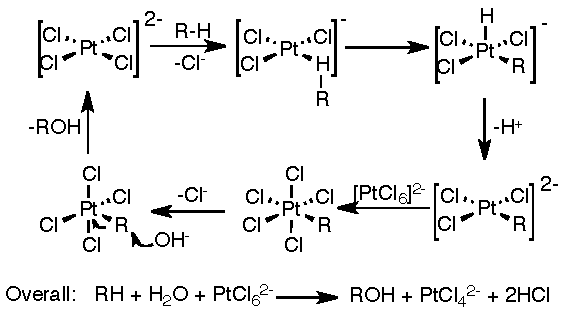
\includegraphics[]{../Schemes/Shilovcatalyticcycle.pdf}
%%\caption[Platinum catalysed oxidation of alkanes]{Platinum catalysed oxidation of alkanes}
%%\label{Shilovcatalyticcycle}
%%\end{scheme}
%%
%%\begin{equation}
%%\ce{CH3CH2OH + H2O + PtCl6}^{2-} \longrightarrow \ce{CH2OHCH2OH + PtCl4}^{2-} + \ce{2HCl} 
%%\label{Ethyleneglycol}
%%\end{equation}
%%
%%Although the Shilov system is catalytic in Pt(II), it requires a stoichiometric amount of Pt(IV).  In addition, the Pt(II) catalyst is unstable in solution and eventually precipitates as platinum metal.\cite{Luinstra1995}  This results in an expensive and thus impractical system for industrial application.  The relatively low yields of the system also reduce its industrial viability.\cite{Periana1993}  Furthermore, the reaction produces two equivalents of hydrochloric acid which require disposal at significant cost.\cite{Poliakoff2001}  A number of attempts have been made to replace the Pt(IV) primary oxidant thus making an economically viable system.\cite{Periana1993, Periana1998, Hashiguchi2010}  However, this has proven challenging as most oxidants tend to convert Pt(II) to the inactive Pt(IV).\cite{Crabtree2001}  Additionally, an oxidant is required that will not attack the product alcohol.  
%%
%%In 1993 Periana reported the use of concentrated sulfuric acid as the primary oxidant and Hg(II) as a catalyst in place of the platinum.\cite{Periana1993}  The Hg(II) is the highest possible oxidation state so further unwanted oxidation of the catalyst is not possible.  Using methane as the feedstock, the system produces methyl bisulfate in a 43\% yield (Scheme \ref{Mercurycatalyticcycle}).  This has the advantage of being highly resistant to oxidation preventing the formation of carbon dioxide. However, the catalysis involves the formation of MeHg(II)$^+$ as an intermediate following activation.  Methyl mercury salts, like most organomercury compounds, are extremely toxic and exhibit accumulation effects in biological systems.\fixme{cite(MethylmercuryMSDS)}  Sulfur dioxide, a significant contributor to acid rain,\cite{Jacobs1999} is also produced as a stoichiometric byproduct of this reaction.  However, the oxidation of sulfur dioxide to sulfuric acid by air is an established industrial process and could be utilised to provide further sulfuric acid for the process.\cite{Periana1993}
%%
%%%\begin{equation}
%%%\ce{CH4 + 2H2SO4} \longrightarrow \ce{CH3OSO3H + 2H2O + SO2} 
%%%\label{Mercuryequation}
%%%\end{equation}
%%
%%%Periana 1993 reaction is carried out at 180 degrees
%%%Periana 1998 reaction is carried out at 100 degrees
%%
%%\begin{scheme}[ht]
%%\centering
%%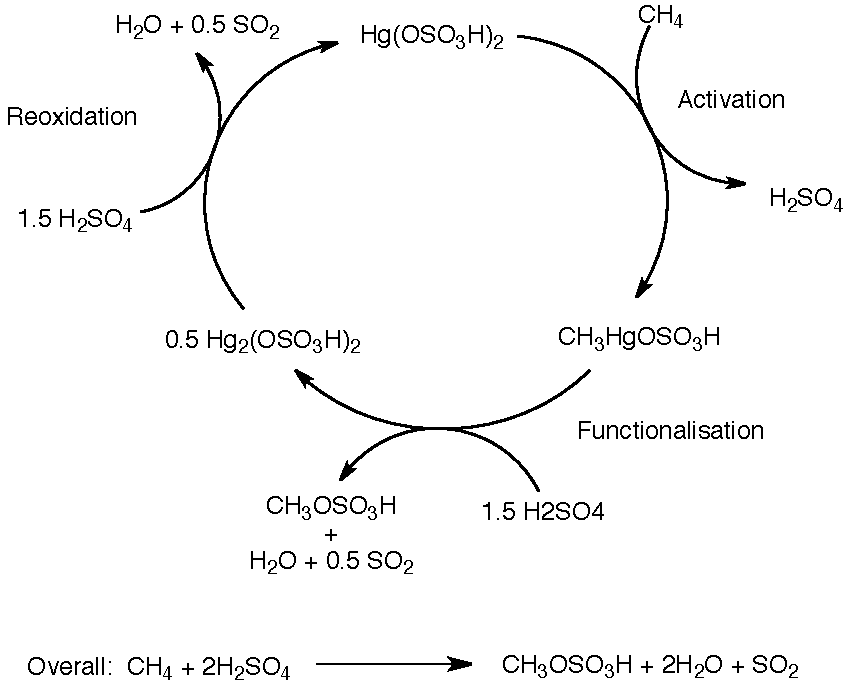
\includegraphics[width = 0.8\textwidth]{../Schemes/Mercurycatalyticcycle.pdf}
%%\caption[Mercury catalysed oxidation of methane]{Mercury catalysed oxidation of methane}
%%\label{Mercurycatalyticcycle}
%%\end{scheme}
%%
%%Further work by Periana investigated changing the Pt(II) system to improve stability, activity and prevent oxidation to Pt(IV).\cite{Periana1998}  Nitrogen donor ligands were utilised as oxygen systems have high kinetic lability on platinum and phosphorus ligands have poor oxidative and thermal stability.  The use of \emph{cis}- or \emph{trans}-\ce{[PtCl2(NH3)2]} in concentrated sulfuric acid at 180~\degrees C gave 90\% selectivity for methyl bisulfate.  However, the catalyst degraded to insoluble \ce{PtCl2} and \ce{NH4HSO4}.  
%%
%%In an extension of this work a $\pi$-acidic chelating donor ligand \gls{bpym} was utilised as $\pi$-donor ligands were expected to have lower proton affinity and form stronger Pt-N bonds than the \ce{NH3} ligands used previously.  The \ce{[PtCl2(}\gls{bpym})] complex was tested in 20 \% \ce{SO3} in \ce{H2SO4} at 200~\degrees C for 50 hours.  Some free ligand and HCl was observed, however the solution remained homogenous showing no formation of platinum metal or other insoluble products.  Using \emph{cis}-\ce{[PtCl2(}\gls{bpym})] in the catalytic system at 220~\degrees C for 2.5 hours resulted in 90\% methane conversion with an 81\% selectivity (carbon dioxide forming the major byproduct).\cite{Periana1998}  However, this reaction requires high temperatures and forms significant amounts of carbon dioxide and sulfur dioxide both of which are environmentally hazardous.\cite{Jacobs1999}  The reaction proceeds \emph{via} a slightly different mechanism to the mercury system (Scheme \ref{PerianaPtcycle}) with oxidation occurring prior to the functionalisation.\cite{Periana1998}
%%
%%%\begin{figure}[h]
%%%\centering
%%%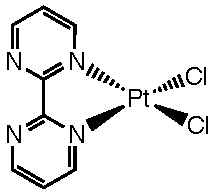
\includegraphics[height = 4cm]{../Figures/bpym.pdf}
%%%\caption[Structure of \ce{[PtCl2(bpym)]}]{Structure of \ce{[PtCl2(bpym)]}}
%%%\label{bpym}
%%%\end{figure}
%%
%%\begin{scheme}[ht]
%%\centering
%%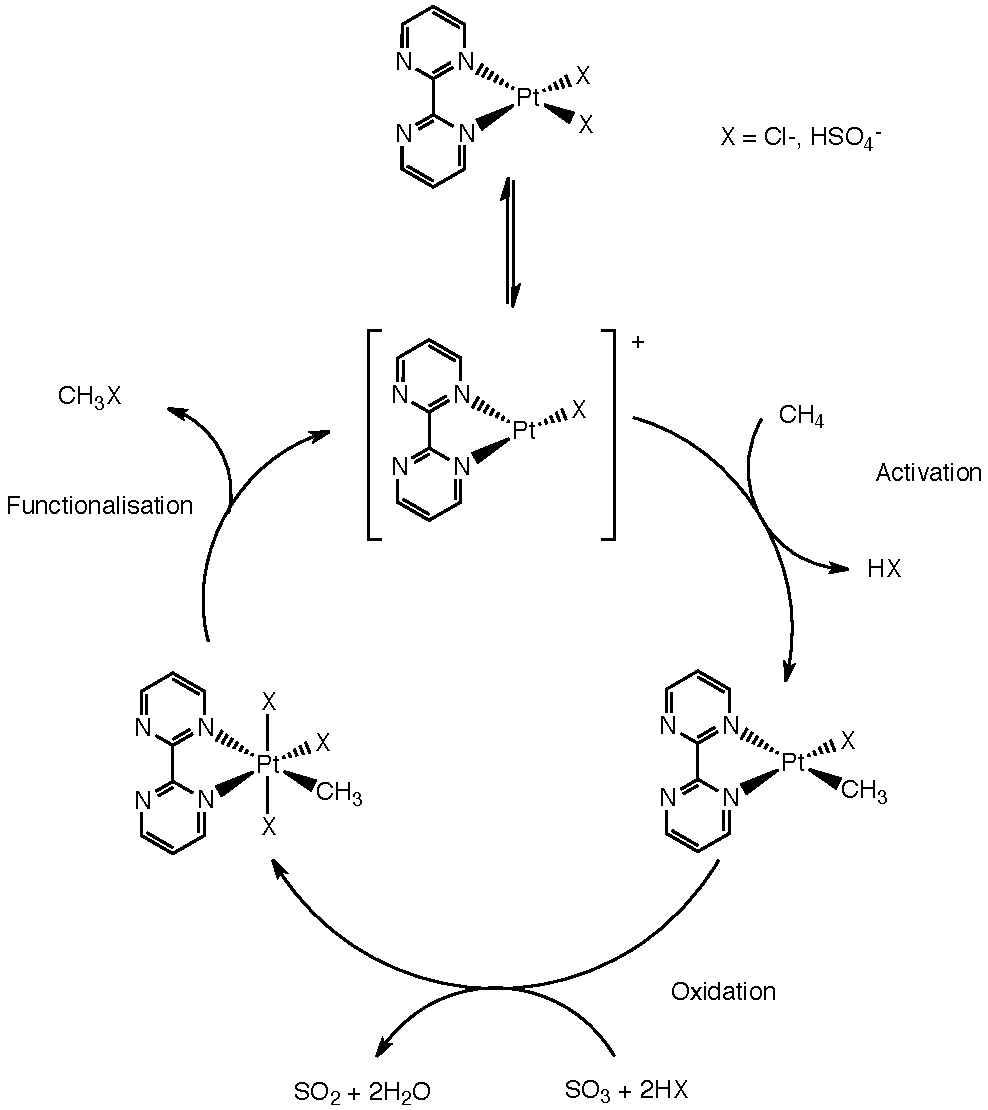
\includegraphics[width = 0.9\textwidth]{../Schemes/PerianaPtcycle.pdf}
%%\caption[Oxidation of methane catalysed by \ce{[PtCl2(bpym)]}]{Oxidation of methane catalysed by \ce{[PtCl2(bpym)]}}
%%\label{PerianaPtcycle}
%%\end{scheme}
%%
%%%Nature of the C-H bond\\ 
%%%Strong\\
%%%Highly non-polar\\
%%%General catalytic attempts\\
%%%Shilov etc.\\
%%
%%\subsection{Alkane dehydrogenation}
%%
%%Alkane dehydrogenation is an alternative approach that combines the activation and functionalisation into a single step.  This methodology was developed from the \hbox{organometallic} complexes such as Wilkinson's\cite{Osborn1966} and Crabtree's\cite{Crabtree1979b} catalysts (Figure \ref{Wilkinsoncrabtree}) that are utilised as homogeneous hydrogenation catalysts.  Wilkinson's catalyst was the first homogeneous hydrogenation catalyst with comparable rates to the heterogeneous counterparts and has become very widely utilised in organic synthesis.\cite{Knowles2003}
%%
%%\begin{figure}[ht]
%%\centering
%%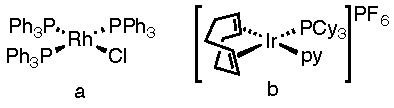
\includegraphics[]{../Figures/Wilkinsoncrabtree.pdf}
%%\caption[Wilkinson's and Crabtree's catalysts]{Wilkinson's (a) and Crabtree's (b) catalysts}
%%\label{Wilkinsoncrabtree}
%%\end{figure}
%%
%%Crabtree reported a number of hydrogenation catalysts based on Wilkinson's catalyst in 1977.\cite{Crabtree1977} The most active of these, \ce{[Ir(cod)(PCy3)(py)]PF6} (Figure \ref{Wilkinsoncrabtree} b, \gls{cod} = 1,5-cyclooctadiene, \gls{Cy}~=~cyclohexyl, \gls{py} = pyridyl) has become known as Crabtree's catalyst.\cite{Cui2005}  This catalyst is active for the hydrogenation of a range of \hbox{mono-,} di-, \hbox{tri-,} and \hbox{tetra-substituted} alkenes with turnover frequencies (\glspl{TOF}) of 6400, 4500, 3800 and 4000 for hex-1-ene, cyclohexene, 1-methylcyclohexene and 2,3-dimethylbut-2-ene respectively.\cite{Crabtree1979b}  Crabtree's catalyst is useful for the hydrogenation of tri- and tetra-substituted alkenes for which Wilkinson's catalyst is inactive.\cite{Cui2005}
%%
%%A catalytic system lowers the activation energy for a reaction, hence both the forward and reverse reactions will be catalysed.\cite{Crabtree2001}  This realisation led Crabtree to test an iridium system for dehydrogenation of alkenes.\cite{Crabtree1979}  The dehydrogenation would normally be strongly endothermic so the substrates were chosen to give products that would bind strongly to the metal to improve the thermodynamics of the reaction.  In the presence of \ce{[IrH2(alkene)2(PPh3)2]+} and 3,3-dimethylbut-1-ene (as hydrogen acceptor) the dehydrogenation of cyclooctene, [2.2.2]bicyclooctene, cyclopentene and cyclohexene were carried out successfully to give complexes of the type \ce{[Ir(diene)(PPh3)2]+} and \ce{[Ir(Cp)H(PPh3)]+} (Cp = cyclopentadienyl).\cite{Crabtree1979}  The dehydrogenation of alkanes was also possible with the system.  The dehydrogenation of cyclopentane to form the cyclopentadienyl complex gave a 30\% yield after 18 hours, whilst the dehydrogenation of cyclooctane to the cyclooctadiene complex gave a 70\% yield after only 4 hours.\cite{Crabtree1979}
%%
%%Felkin reported a rhenium complex capable of dehydrogenating linear alkanes to dienes.\cite{Baudry1982}  In the presence of \ce{[ReH7(PAr3)2]} (Ar = \emph{p}-\ce{MeC6H4}) and 3,3-dimethylbut-1-ene, \emph{n}-pentane was dehydrogenated to form a diene complex (Scheme \ref{Pentanedehydrogenation}).  Treatment of this complex with \ce{P(OMe)3} produced pent-1-ene with a yield of 45\%.  This was extended to the linear isomers of hexane, heptane and octane.\cite{Baudry1984}  Although pentane can form only one conjugated diene complex, hexane and heptane can give two, whilst octane can give three.  However, in all cases upon treatment of the complex with \ce{P(OMe)3} the terminal alkene was formed with a selectivity of over 95\%.\cite{Baudry1984}  
%%
%%\begin{scheme}[ht]
%%\centering
%%\includegraphics[]{../Schemes/Pentanedehydrogenation.pdf}
%%\caption[Dehydrogenation of pentane]{Dehydrogenation of pentane reproduced from Felkin et al.\cite{Baudry1982}}
%%\label{Pentanedehydrogenation}
%%\end{scheme}
%%
%%Wilkinson's catalyst (figure \ref{Wilkinsoncrabtree}b) has also been utilised as a dehydrogenation catalyst.\cite{Fujii1990}  The dehydrogenation of cyclooctane to give cyclooctene by \ce{[RhCl(L)3]} (L = \ce{PPh3} or P(\emph{p}-\ce{tolyl)3}) was carried out at reflux (151~\degrees C) without the need for a hydrogen acceptor.  The high temperature of the reaction mixture is sufficient to allow the removal of molecular hydrogen from the reaction mixture.\cite{Fujii1990}  The reaction rates obtained with this system were low, the highest with L = P(\emph{p}-\ce{tolyl)3} was only 1.24 h\ce{^{-1}} with a L/Rh ratio of 8.\cite{Fujii1990}
%%
%%Crabtree utilised this acceptorless methodology to test the catalytic activity of iridium complexes.\cite{Aoki1993}  \ce{[IrH2L(PCy3)2]} (L = \ce{O2CCF3}, \ce{O2CC2F5} and \ce{O2CPhCH2}) were active for the dehydrogenation of cyclooctane under reflux with initial turnover frequencies of 1.41, 1.05 and 0.22 \ce{h^{-1}} respectively.  However, the complexes were unstable with deactivation half lives of 15, 34 and 14 hours respectively.\cite{Aoki1993}  Alternate methods to remove the hydrogen were also tested.  Using perfluorodecalin as a solvent allowed for more effective hydrogen removal due to the higher volatility compared to cyclooctane.  This resulted in poor activity with a turnover frequency of 0.24 \ce{h^{-1}} using \ce{[IrH2(O2CCF3)(PCy3)2]} as catalyst.  Bubbling inert gas was unsuccessful with cyclooctane as a substrate as a large amount of the substrate was lost.  However, using the less volatile cyclodecane a turnover frequency of 0.48 \ce{h^{-1}}  was obtained.\cite{Aoki1993}
%%
%%%\fixme{Goldman reference 4 from Gupta1996 had an improved non-pincer system}
%%
%%\section{Pincer ligands}
%%
%%Recently, the so-called pincer ligands have attracted a great deal of research attention due to their unique balance of stability and reactivity.\cite{Becerra2009}  Pincer ligands are tridentate ligands that bind in a meridional fashion, examples of which are given in Figure \ref{Pincernaming}.  Pincer ligands are named based on their donor atoms such as, PCP, NCN, and POP.  If the groups between the donor atoms contain heteroatoms then these may be included in the naming also, for example POCOP.  The pincer ligands may be anionic (as with PCP ligands) or neutral (PNP and POP).\cite{Vlugt2009, Kataoka1995}  Although phosphines are the most common donor groups, amines,\cite{Singleton2003} imines,\cite{Takenaka2005} thioethers\cite{Zim2000} and N-heterocyclic carbenes\cite{Hahn2007} have all been reported.
%%
%%\begin{figure}[ht]
%%\centering
%%\includegraphics[]{../Figures/Pincernaming.pdf}
%%\caption[Naming of pincer ligands]{Naming of pincer ligands}
%%\label{Pincernaming}
%%\end{figure}
%%
%%The first reports of pincer ligands were in 1976 by Shaw\cite{Moulton1976} and Alcock.\cite{Alcock1976}  Shaw reported a \emph{tert}-butyl PCP ligand (Figure \ref{Shaw}) and introduced the naming scheme that has become commonplace for pincer ligands.  When reacted with an appropriate metal precursor, complexes formed between the tridentate ligand with nickel, palladium, platinum, rhodium and iridium with chloride, nitrile, hydride and carbon monoxide ligands.\cite{Moulton1976} 
%%
%%\begin{figure}[ht]
%%\centering
%%\includegraphics[]{../Figures/Shaw.pdf}
%%\caption[First reported PCP pincer ligand]{First reported PCP pincer ligand}
%%\label{Shaw}
%%\end{figure}
%%
%%Alcock reported X-ray crystal structures of the first complexes of POP ligands (Figure \ref{Alcock}).\cite{Alcock1976}  These formed rhodium carbonyl complexes that were characterised by X-ray crystallography.  With a single ether group in the backbone it forms a typical pincer complex, bonding through the phosphorus and oxygen atoms.  However, when there are three ether units the phosphorus atoms bond to the rhodium but the oxygen H-bonds to a water molecule that is bound to the rhodium centre.\cite{Alcock1976}
%%
%%\begin{figure}[ht]
%%\centering
%%\includegraphics[]{../Figures/Alcock.pdf}
%%\caption[First reported POP pincer ligand]{First reported POP pincer ligand}
%%\label{Alcock}
%%\end{figure}
%%
%%%Typically the central donor atom E is a carbon from an aromatic ring that binds through C-H activation to form a metallacycle.\cite{Choi2011}  
%%
%%The different components of pincer ligands have significant influence on the steric and electronic properties and hence their reactivity.\cite{Singleton2003}  Altering the group X (Figure \ref{Pincerligands}) can lead to significant electronic effects mostly through the \emph{trans} influence.\cite{Choi2011}  For example, a carbon donor ligand has a greater \emph{trans} influence than an oxygen donor, so ligands \emph{trans} to X in PXP complexes will be bound more strongly when X~=~O than X~=~C.\cite{Zhu2008} The donor group Y controls the steric environment around the metal centre and the electron density.\cite{Choi2011}  Changing the backbone and other remote groups gives control over the electron density on the metal and can be used to improve solubility properties.\cite{Choi2011}
%%
%%\begin{figure}[ht]
%%\centering
%%\includegraphics[]{../Figures/Pincerligands.pdf}
%%\caption[General representation of pincer ligands]{General representation of pincer ligands}
%%\label{Pincerligands}
%%\end{figure}
%%
%%The tridentate coordination of pincer ligands, typically forming two five-membered metallacycles, imparts significant stability to metal complexes with pincer ligands.\cite{Choi2011}  The stability of the complexes is such that the backbone can undergo functionalisation at the 4-position to trimethylsilane \emph{via} lithiation with \emph{tert}-butyllithium and treatment with trimethylchlorosilane without inducing any decomposition of the platinum complex (Scheme \ref{Stability}).\cite{Albrecht2001}  This inherent stability allows the complexes to act as catalysts for highly endothermic reactions that require high temperatures, such as alkane dehydrogenation.\cite{Choi2011}
%%
%%\begin{scheme}[ht]
%%\centering
%%\includegraphics[]{../Schemes/Stability.pdf}
%%\caption[Functionalisation of an NCN pincer ligand]{Functionalisation of an NCN pincer ligand}
%%\label{Stability}
%%\end{scheme}
%%
%%Coordination complexes of pincer ligands have a large number of applications.  Platinum complexes of an NCN pincer ligand have been utilised as sensors for the detection of sulfur dioxide.\cite{Albrecht2000, Albrecht2000c, Albrecht2001}  Palladium and nickel complexes of a number of pincer ligands have shown activity in cross-coupling reactions.\cite{Hahn2007, Bedford2000, Kimura2006, Zim2000, Obora2006} Theoretical studies have shown potential uses for pincer ligands in water-splitting\cite{Sandhya2011} and nitrogen fixation.\cite{Holscher2007}  However, one of the most prominent uses of pincer ligands is the activation of C-H bonds, typically as dehydrogenation catalysts.\cite{Choi2011, Albrecht2001, Crabtree2001}
%%
%%%\subsection{Gas sensors}
%%
%%%Platinum complexes of an NCN pincer (Figure \ref{Gassensors} \fixme{reference the structure correctly}) have been studied in solution or the crystalline state for use in the detection of sulfur dioxide.\cite{Albrecht2000, Albrecht2000c, Albrecht2001b}  In the presence of sulfur dioxide the square planar complex rapidly (less than 50 \si{\micro\second} adsorb the gas to form square pyramidal structures.\cite{Albrecht2000}  The adsorption is accompanied by a dramatic colour change from colourless to bright orange and is reversible upon exposure to a sulfur dioxide free atmosphere.\cite{Albrecht2000}  Dendrimer derivatives (2 and 3, Figure \ref{Gassensors}) can be used to detect sulfur dioxide at concentrations as low as 5 ppm (in a nitrogen atmosphere) \cite{Albrecht2001b}  
%%
%%%\begin{figure}[h]
%%%\centering
%%%\includegraphics[width = \textwidth]{../Figures/Gassensors.pdf}
%%%\caption[NCN platinum complexes used for sensing \ce{SO2}]{NCN platinum complexes used for sensing \ce{SO2}}
%%%\label{Gassensors}
%%%\end{figure}
%%
%%%These sensors have been studied further for physiological applications.  The complex (Figure \ref{Physiologicalgassensors}) is stable in both acidic and basic aqueous solutions for prolonged periods.\cite{Albrecht2000b}  Testing in conditions known to lead to rapid protein degradation (pH < 1, 50 \degrees C, 5 hours) results in no detectable decomposition.\cite{Albrecht2000b}  The coordination of sulfur dioxide to the complex results in a large shift in the $^{195}$Pt NMR of 1150 ppm (from -3150 to -2000 ppm).\cite{Albrecht2000b}  This could be detected by MRI for medical applications.  These complexes are also being developed for use as molecular switches for opto-electronics.\cite{Albrecht2000c}
%%
%%%\begin{figure}[h]
%%%\centering
%%%\includegraphics[height = 4.5cm]{../Figures/Physiologicalgassensors.pdf}
%%%\caption[NCN platinum complexes developed for \ce{SO2} sensing in physiological settings]{NCN platinum complexes developed for \ce{SO2} sensing in physiological settings}
%%%\label{Physiologicalgassensors}
%%%\end{figure}
%%
%%%\subsection{Cross-coupling reactions}
%%
%%%Coordination complexes of pincer ligands also find use as catalysts in carbon-carbon cross-coupling reactions such as the Suzuki, Heck \fixme{etc}.
%%
%%%Pincer ligands with N-heterocyclic carbene (NHC) donors are becoming more common.\fixme{reference}  The palladium complexes found in figure \ref{CCCPincers} are active for the heck cross-coupling reaction of aryl bromides with styrene and the suzuki cross-coupling of aryl bromides with phenylboronic acid.\cite{Hahn2007}  Using a 1 mol \% catalyst loading the reaction of 4-bromobenzaldehyde and 4-bromoacetophenone with styrene quantitative yields were obtained after 24 hours regardless of the substituent on the ligand.  Using the \emph{n}-butyl derivatised ligand after two hours yields of 84.1, and 60.0 \% were obtained for reaction of styrene with 4-bromobenzaldehyde and 4-bromoacetophenone respectively.   The \emph{n}-butyl derived ligand formed an active palladium catalyst for the Suzuki cross-coupling of phenylboronic acid with 4-bromobenzaldehyde and 4-bromoacetophenone.  Using a 0.1 \% catalyst loading  yields of 50.7 and 48.7 \% respectively were obtained after two hours and quantitative conversion obtained in 24 hours.
%%
%%%\begin{figure}[h]
%%%\centering
%%%\includegraphics[height = 6 cm]{../Figures/CCCPincers.pdf}
%%%\caption[Palladium complexes with NHC donor pincer ligands]{Palladium complexes with NHC donor pincer ligands}
%%%\label{CCCPincers}
%%%\end{figure}
%%
%%%The palladium complexes with ferrocene based PCP ligands (figure \ref{Ferrocenepalladium}) have been tested for activity in the Suzuki cross-coupling reaction.\cite{Sheloumov2008}  After 4.5 hours the reaction of 4-bromoacetophenone with phenylboronic acid in the presence of 1 and 3 was almost complete with 84 and 84.5 \% yields respectively under homogeneous conditions and quantitative yields under biphasic conditions (decane/\ce{H2O}).  The reaction was much slower with complex 2 with only 66 \% obtained after 15 hours.  Similar activities for all complexes were obtained for the homogeneous reaction of phenylboronic acid with 4-bromoanisole with yields of 77, 79 and 98 \% after 12, 15 and 15.5 hours for 1, 2 and 3 respectively.  However under biphasic conditions complex 2 was much less reactive obtaining a yield of 9 \% after 15 hours compared to 62 and 63.5 \% for 1 and 3 respectively.  The lower activity for complex 2 is thought to be due to the steric bulk of the \emph{tert}-butyl groups though in complex 3 the steric effect is overcome by the electronic influence of the Fe(III) rather than Fe(II).\cite{Sheloumov2008}
%%
%%%See 
%%
%%%\begin{figure}[h]
%%%\centering
%%%\includegraphics[height = 4.5cm]{../Figures/Ferrocenepalladium.pdf}
%%% \caption[Palladium complexes of ferrocene pincer ligands]{Palladium complexes of ferrocene pincer ligands}
%%%\label{Ferrocenepalladium}
%%%\end{figure}
%%
%%%Definition\\	
%%%Naming\\
%%%Uses of the ligands\\
%%%Gas sensors\\
%%%SO2\\
%%%PCP\\
%%%POCOP\\
%%%PNP\\
%%%POP\\
%%%Nitrogen activation and fixation\\
%%
%%\subsection{C-H activation}
%%%\subsection{Alkane dehydrogenation}
%%
%%The catalytic dehydrogenation of alkanes has the potential to develop into an important industrial process allowing alkanes to be used as a chemical feedstock, without requiring high temperature cracking or other inefficient processes.\cite{Choi2011}  The first use of pincer complexes for alkane dehydrogenation was reported by Gupta in 1996.\cite{Gupta1996}  The rhodium and iridium dihydride complexes in figure \ref{Dehydrogenationligands} were tested for the dehydrogenation of cyclooctane in the presence of 3,3-dimethylbut-1-ene as hydrogen acceptor.  Rates of 0.8 turnovers h$^{-1}$ at 150~\degrees C were obtained for the rhodium complex, whilst the iridium complex was more active with rates of 82 turnovers h$^{-1}$.\cite{Gupta1996}  The catalysts used were highly stable at this temperature for extended periods and the addition of mercury did not inhibit the reaction indicating a homogeneous system.\cite{Gupta1996}  The higher activity of the iridium complex combined with the high thermal stability has led to a focus on iridium complexes for alkane dehydrogenation.\cite{Choi2011}
%%
%%\begin{figure}[ht]
%%\centering
%%\includegraphics[]{../Figures/Dehydrogenationligands.pdf}
%%\caption[Rhodium and iridium pincer complexes used for alkane dehydrogenation]{Rhodium and iridium pincer complexes used for alkane dehydrogenation}
%%\label{Dehydrogenationligands}
%%\end{figure}
%%
%%The iridium complex (Figure \ref{Dehydrogenationligands}) was also active for the dehydrogenation of cyclic alkanes, tetrahydrofuran and ethylbenzene to give arenes, furan and styrene respectively.\cite{Gupta1997, Gupta1997b}  In all cases the presence of excess 3,3-dimethylbut-1-ene as hydrogen acceptor inhibited the reaction so it was necessary to add this periodically.  A nitrogen atmosphere also inhibited reaction indicating competitive binding of nitrogen and alkane to the active site.\cite{Gupta1996, Gupta1997, Gupta1997b}  The iridium complex is also active for the dehydrogenation of cyclooctane and cyclodecane under acceptorless conditions.\cite{Xu1997}  A solution of fresh catalyst could be poisoned by addition of 10\% alkene rendering the catalyst inactive and indicating that the reduction of activity over time is not due to catalyst decomposition.\cite{Xu1997}
%%
%%A mechanism for the alkane transfer dehydrogenation (Scheme \ref{Dehydrogenationcatalyticcycle}) has been elucidated \emph{via} a kinetics study by Goldman.\cite{Renkema2003}  The 3,3-dimethylbut-1-ene inserts into an iridium hydride bond, which is followed by reductive elimination to give the alkane.  The substrate undergoes oxidative addition to the iridium centre, which is followed by $\beta$-hydride elimination to give the alkene product and regenerate the iridium-dihydride.  With a limited concentration of 3,3-dimethylbut-1-ene (as is typical for these reactions) the rate determining step is the hydrogenation of the acceptor rather than C-H activation of the alkane, however with an excess of acceptor the rate determing step is the reaction with the cyclooctane.\cite{Renkema2003}  
%%
%%\begin{scheme}[ht]
%%\centering
%%\includegraphics[]{../Schemes/Dehydrogenationcatalyticcycle.pdf}
%%\caption[Proposed mechanism for transfer dehydrogenation]{Proposed mechanism for transfer dehydrogenation}
%%\label{Dehydrogenationcatalyticcycle}
%%\end{scheme}
%%
%%The three-coordinate [Ir(PCP)] intermediate formed following C-H elimination (Figure \ref{Dehydrogenationcatalyticcycle}) was proposed on the basis of an NMR study showing that the dihydride complex will react with 3,3-dimethylbut-1-ene to give the \emph{trans}-2-(\emph{tert}-butyl)vinyl complex that is in equilibrium with [Ir(PCP)] on an NMR timescale.\cite{Kanzelberger2000}  A more recent study has reported this resting state of the complex as the $\pi$-alkene complex and it is likely that both occur depending on the concentration of the hydrogen acceptor.\cite{Choi2011}  Studies into the acceptorless reaction have shown a similar mechanism.\cite{Krogh2002, Krogh2002b}  In this case the rate determining step is the thermolytic loss of \ce{H2} to give the active dehydrogenation complex [Ir(PCP)].  The inhibition of activity resulting from a build-up of alkene is likely due to the formation of the $\pi$-alkene complex and increased rate of the reverse reaction.\cite{Krogh2002, Krogh2002b}
%%
%%Introduction of electron-donating groups such as \ce{OCH3} in the \emph{para}-position (Figure \ref{DFTpincers}) was shown to favour oxidative addition of an alkane to the 14-electron [Ir(PCP)] complex whilst disfavouring further addition of alkane to the \ce{[(PCP)Ir(R)(H)]} complex.\cite{Krogh2002c}  In the acceptorless dehydrogenation of cyclodecane at reflux (201 \degrees C) the electron-donating \ce{OCH3} pincer complex achieved 820 turnovers in 48 hours compared to 360 with a hydrogen in the \emph{para}-position.\cite{Zhu2004}   However, in dehydrogenation of \emph{n}-undecane at 196 \degrees C little difference was seen between the H and \ce{OCH3} substituted ligands with turnovers of 76 and 91 respectively after 4 hours.  The less sterically bulky isopropyl derivative (with \ce{OCH3} in the \emph{para}-position) was also tested and achieved 2970 turnovers over 48 hours for the dehydrogenation of cyclodecane, indicating that the steric bulk of the ligand has a significant influence of the rate of reaction.\cite{Zhu2004}   In the dehydrogenation of \emph{n}-undecane at 196~\degrees C the isopropyl catalyst was much less active than the \emph{tert}-butyl with only 30 turnovers achieved after 4 hours.  	
%%
%%\begin{figure}[ht]
%%\centering
%%\includegraphics[]{../Figures/DFTpincers.pdf}
%%\caption[Electron-donating pincer ligands]{Electron-donating pincer ligands}
%%\label{DFTpincers}
%%\end{figure}
%%
%%The steric environment imposed by the pincer ligand has a significant impact on the activity towards alkane dehydrogenation.\cite{Choi2011}  A computational and experimental study into this effect was reported by Brookhart in 2009.\cite{Kundu2009}  By exchanging the \emph{tert}-butyl groups on the xylene based PCP complex for methyl groups the impact of the sterically bulky \emph{tert}-butyl groups on alkane dehydrogenation could be studied.  Exchanging a single \emph{tert}-butyl results in a decrease in the transition state for the rate determining step ($\beta$-H elimination) of 42 kJmol$^{-1}$.  This was offset slightly by an increase of 17 kJmol$^{-1}$ in the bond strength of but-1-ene to the iridium centre.  Exchanging a second \emph{tert}-butyl for a methyl was calculated to have a much smaller overall impact as the but-1-ene bonds much more strongly to the metal centre.\cite{Kundu2009}  These results were supported experimentally in the transfer dehydrogenation of \emph{n}-octane using 3,3-dimethylbut-1-ene as the acceptor.  With one and two methyls replacing \emph{tert}-butyl groups, 195 and 140 turnovers were obtained respectively, compared to only 53 for the unmodified ligand.\cite{Kundu2009}
%%
%%Although the PCP iridium complexes are stable at 150 \degrees C for extended periods, significant decomposition becomes apparent after 24 hours at 200 \degrees C.\cite{Gupta1996}  Ligands based on an anthracene backbone (Figure \ref{Anthraphos}) were developed to achieve a higher level of thermal stability.\cite{Haenel2001}  The ``anthraphos'' ligand forms thermally stable complexes with decomposition occurring at 308 \degrees C for the iridium dihydride complex.  However, in the catalytic dehydrogenation of cyclodecane at 150 \degrees C the complex was less active than the xylene-based systems.  It was proposed that the lack of flexibility in the backbone of anthraphos was responsible for the decreased activity.\cite{Haenel2001}
%%
%%\begin{figure}[ht]
%%\centering
%%\includegraphics[]{../Figures/Anthraphos.pdf}
%%\caption[Iridium anthraphos complexes tested for catalytic dehydrogenation]{Iridium anthraphos complexes tested for catalytic dehydrogenation}
%%\label{Anthraphos}
%%\end{figure}
%%
%%The bis-phosphinite (POCOP) pincer ligands in Figure \ref{Phosphinite} were reported independently by Brookhart (R = \ce{^{t}Bu}, X = \ce{OCH3}, \ce{CH3}, H, F, \ce{C6F5}, ArF)\cite{Gottker2004, Gottker2004b} and Jensen (R~=~\ce{^{i}Pr}, X = H) in 2004.\cite{Morales2004}  Brookhart's complexes were tested for activity in the transfer dehydrogenation of cyclooctane at 200 \degrees C using 3,3-dimethylbut-1-ene as hydrogen acceptor.  These complexes displayed high turnover numbers of up to 2041 after 40 hours forming both cyclooctene and 1,3-cyclooctadiene.\cite{Gottker2004}  The cyclooctadiene product spontaneously converts (most likely \emph{via} a disrotatory ring closure of cyclooctatriene) into \emph{o}-xylene and ethylbenzene (Scheme \ref{Benzeneformation}).\cite{Gottker2004}
%%
%%\begin{figure}[ht]
%%\centering
%%\includegraphics[]{../Figures/Phosphinite.pdf}
%%\caption[Iridium POCOP complex]{Iridium POCOP complex}
%%\label{Phosphinite}
%%\end{figure}
%%
%%\begin{scheme}[ht]
%%\centering
%%\includegraphics[]{../Schemes/Benzeneformation.pdf}
%%\caption[Reaction of cyclooctene to form alkylbenzenes]{Reaction of cyclooctene to form alkylbenzenes}
%%\label{Benzeneformation}
%%\end{scheme}
%%
%%The electronic influence of the pincer ligand can also have a dramatic impact on the catalytic activity.  A ruthenium PCP complex with electron-withdrawing \ce{CF3} substituents on the phosphorus atoms (Figure \ref{ElectronwithdrawingPCP}) was tested for transfer and acceptorless dehydrogenation of cyclooctane.\cite{Gruver2011}  The catalyst achieved 186 turnovers at 200 \degrees C after only 30 minutes of transfer dehydrogenation and 10 turnovers in 60 minutes under acceptorless conditions.  This complex was prone to decomposition due to the high temperatures used.  However, the presence of oxygen, nitrogen and water resulted in no significant change to the catalysis which is a significant advantage over other systems.  
%%
%%\begin{figure}[ht]
%%\centering
%%\includegraphics[]{../Figures/ElectronwithdrawingPCP.pdf}
%%\caption[Ruthenium complex of an electron-withdrawing PCP ligand]{Ruthenium complex of an electron-withdrawing PCP ligand}
%%\label{ElectronwithdrawingPCP}
%%\end{figure}
%%
%%Pincer complexes based on metallocenes have also been synthesised and tested for use in alkane dehydrogenation (Figure \ref{Metallocenepincers}).\cite{Kuklin2006}  These complexes have much higher activity than those previously reported.  Turnover numbers of 3300 and 2571 were obtained after eight hours for the iron and ruthenium metallocenes, respectively in the transfer dehydrogenation of cyclooctane with 3,3-dimethylbut-1-ene as hydrogen acceptor at 180 \degrees C.  This compares with 1843 for the iridium POCOP pincer complex (Figure \ref{Phosphinite}) when tested in the same conditions.  The increased activity was proposed as being due to less steric hindrance of the metal centre compared to the POCOP complex.\cite{Kuklin2006}
%%
%%\begin{figure}[ht]
%%\centering
%%\includegraphics[]{../Figures/Metallocenepincers.pdf}
%%\caption[Metallocene based pincer ligands]{Metallocene based pincer ligands}
%%\label{Metallocenepincers}
%%\end{figure}
%%
%%\subsection{Alkane metathesis}
%%
%%Alkene metathesis is a well-known chemical transformation where the groups of two alkenes are exchanged in the presence of an appropriate catalyst.\cite{Astruc2005}  Alkane metathesis follows the same general principle; the exchange of alkane fragments to produce an array of longer and shorter alkanes.\cite{Choi2011}  Although this was first studied from a heterogeneous perspective,\cite{Burnett1973, Vidal1997, Basset2005} more recently homogeneous pincer complexes have been utilised.\cite{Goldman2006}
%%
%%%Shell higher olefins process
%%
%%The first alkane metathesis catalysts were heterogeneous mixtures of dehydrogenation/ hydrogenation and metathesis catalysts.\cite{Burnett1973, Vidal1997}   A mixture of tungsten oxide on silica and platinum metal on alumina formed an active alkane metathesis catalyst.\cite{Burnett1973}  The platinum metal dehydrogenates the alkane, which then reacts in an alkene metathesis reaction, followed by hydrogenation by the platinum to form shorter and longer alkanes.  When exposed to \emph{n}-butane a mixture of 24.7, 37.6, 15.9 and 8.6\% of \ce{C3}, \ce{C4}, \ce{C5} and \ce{C6} linear alkanes was obtained with small amounts of branched and higher alkanes.  However, this system required high temperature (400 \degrees C) and was very sensitive to poisoning by water, ammonia, oxygen and hydrogen sulfide.\cite{Burnett1973}
%%
%%A tantalum hydride catalyst on silica was more successful with catalysis occuring at room temperature.\cite{Vidal1997}  This system followed a slightly different mechanism, shown in Scheme \ref{Tantalumcatalyticcycle}.  The first step involves coordination to the tantalum \emph{via} loss of hydrogen gas.  This is followed by addition of further alkane to form a metallacycle intermediate that rearranges to give the longer chain product and a tantalum methyl species.  This can react with further alkane to form methane and regenerate the catalytic tantalum alkyl species.  This system is active towards a number of alkanes giving a statistical distribution of longer and shorter alkanes, however the turnover numbers obtained were low; 46, 47, 66, 17 and 12 for ethane, propane, butane, isobutane and pentane respectively.\cite{Vidal1997}
%%
%%\begin{scheme}[ht]
%%\centering
%%\includegraphics[width = 0.7\textwidth]{../Schemes/Tantalumcatalyticcycle.pdf}
%%\caption[Catalytic cycle for alkane metathesis by a heterogeneous tantalum catalyst]{Catalytic cycle for alkane metathesis by a heterogeneous tantalum catalyst}
%%\label{Tantalumcatalyticcycle}
%%\end{scheme}
%%
%%The use of pincer complexes for alkane metathesis has typically followed the tandem alkane dehydrogenation and alkene metathesis protocol (Scheme \ref{Tandemmetathesis}).\cite{Choi2011} Combining an iridium pincer dehydrogenation catalyst with the Schrock alkene metathesis catalyst (Figure \ref{PCPSchrock}) gave active catalysts with turnover numbers of 135, 205 and 125 after 24 hours for the conversion of \emph{n}-hexane using pincer complexes (a) (with L = \ce{C2H4}, \ce{H2}) and (b) respectively.\cite{Goldman2006}  The activity was limited by degradation of the alkene metathesis catalyst as reaction resumed upon further addition of Schrock's catalyst.  A major advantage of this catalytic system is the selective formation of linear alkanes as no branched or cyclic alkanes were detected.\cite{Goldman2006}
%%
%%\begin{scheme}[ht]
%%\centering
%%\includegraphics[]{../Schemes/Tandemmetathesis.pdf}
%%\caption[Alkane metathesis \emph{via} transfer hydrogenation and alkene metathesis]{Alkane metathesis \emph{via} transfer hydrogenation and alkene metathesis}
%%\label{Tandemmetathesis}
%%\end{scheme}
%%
%%\begin{figure}[ht]
%%\centering
%%\includegraphics[]{../Figures/PCPSchrock.pdf}
%%\caption[Transfer hydrogenation and alkene metathesis catalysts]{Transfer hydrogenation and alkene metathesis catalysts}
%%\label{PCPSchrock}
%%\end{figure}
%%
%%Replacement of Schrock's catalyst with a heterogeneous alkene metathesis catalyst was tested to increase the stability.  This \ce{Re2O7}/\ce{Al2O3} catalyst was more stable than Schrock's catalyst and showed a higher level of activity with 125 turnovers achieved with complex (b) (Figure \ref{PCPSchrock}) and 180 for complex (c) in 3 hours for the conversion of \emph{n}-decane.\cite{Goldman2006}  However, the activity of the phosphinite complexes was reduced with (a) achieving only 15 turnovers in 3 hours.  Although a high level of selectivity with complexes (b) and (c) for terminal alkenes has been reported for the dehydrogenation,\cite{Liu1999} the product distribution (Figure \ref{GCdistribution})  shows no preference for ethane, which would occur if this was the case.  Either isomerisation of the terminal alkene to form internal alkenes prior to metathesis, or further reaction of the alkane products must occur to account for the observed product distribution.\cite{Goldman2006, Choi2011}
%%
%%\begin{figure}[ht]
%%\centering
%%\includegraphics[width = 0.65\textwidth]{../Figures/GCdistribution.pdf}
%%\caption[GC trace of products obtained from alkane metathesis of \emph{n}-decane]{GC trace of products obtained from alkane metathesis of \emph{n}-decane reproduced from Goldman et al.\cite{Goldman2006}}
%%\label{GCdistribution}
%%\end{figure}
%%
%%\subsection{POP pincer ligands}
%%
%%Although one of the first pincer ligands reported was a POP pincer,\cite{Alcock1976} this type of ligand has not been studied as extensively as the PCP and PNP analogues.  The osmium trichloride complex of \gls{dbf}(P$^i$\ce{Pr2)2} (Figure \ref{Osmiumdbf}) formed in 98\% yield when the ligand was reacted with the commercially available \ce{OsCl3}$\cdot{}$3\ce{H2O} under reflux.\cite{Asensio2010}  When the ligand is reacted with \ce{OsCl2(DMSO)4} (DMSO = dimethylsulfoxide) the \emph{trans}-dichloro \gls{DMSO} complex (Scheme \ref{Osmiumdbfscheme}) is formed.\cite{Esteruelas2011} This complex can be converted to trihydridechloride and tetrahydride osmium complexes upon reaction with hydrogen gas in the presence of triethylamine or sodium hydrid,e respectively.  The tetrahydride complex is an active catalyst for the coupling of amines and alcohols to give imines achieving a 98\% yield after 3 hours for the coupling of benzyl alcohol and aniline.  Lower yields of 49 and 54\% were obtained when the \gls{DMSO} and trihydride complexes were used.\cite{Esteruelas2011}
%%
%%\begin{figure}[ht]
%%\centering
%%\includegraphics[]{../Figures/Osmiumdbf.pdf}
%%\caption[Osmium trichloride complex of \ce{dbf(P^{i}Pr2)2}]{Osmium trichloride complex of \ce{dbf(P^{i}Pr2)2}}
%%\label{Osmiumdbf}
%%\end{figure}
%%
%%\begin{scheme}[ht]
%%\centering
%%\includegraphics[]{../Schemes/Osmiumdbfscheme.pdf}
%%\caption[Reaction of osmium complexes of \ce{dbf(P^{i}Pr2)2}]{Reaction of osmium complexes of \ce{dbf(P^{i}Pr2)2}}
%%\label{Osmiumdbfscheme}
%%\end{scheme}
%%
%%A theoretical study has suggested that POP pincers could be utilised as ligands for ruthenium catalysed synthesis of ammonia from nitrogen and hydrogen gases.\cite{Holscher2007}  The PNP and PSP ligands (Figure \ref{Theoreticalammonia}) have much higher activation barriers for the formation of the active catalytic species than the POP ligands.  Theoretical studies into Shilov chemistry have shown that the presence of an oxygen or nitrogen ligand \emph{trans} to the methane results in much lower activation barriers.\cite{Zhu2009}  The two-step process for C-H activation involves the loss of a ligand followed by coordination of the methane.  The C-H activation has no discernible energy barrier when an oxygen ligand is present in the \emph{trans}-position, however the intial loss of the ligand is much faster for ligands with a higher \emph{trans}-influence making the nitrogen donors much better overall.  Given a system where other factors promoted the loss of the ligand (such as steric bulk) it may be possible that the oxygen-donor ligands are better overall.  
%%
%%\begin{figure}[ht]
%%\centering
%%\includegraphics[]{../Figures/Theoreticalammonia.pdf}
%%\caption[Pincer ligands studied for catalytic ammonia synthesis]{Pincer ligands studied for catalytic ammonia synthesis}
%%\label{Theoreticalammonia}
%%\end{figure}
%%
%%Research into the effect of different phosphorus substituents on the reactivity of ruthenium POP pincer complexes has been reported.\cite{Major2005}  Reaction of \ce{[RuCl2(}\emph{p}-\ce{cymene)]2} (\gls{cymene} = 1-methyl-4-(1-methylethyl)benzene) with the sterically bulky POP-\ce{^{t}}Bu yielded the five-coordinate complex, [Ru\ce{Cl2}(POP)] (Scheme \ref{RutheniumPOP}).  However, the less bulky POP-\ce{^{i}Pr} formed a dimeric species.  Both species were able to form molecular hydrogen complexes however, with the POP-\ce{^{i}}Pr, the \ce{H2} occupies the site \emph{trans} to the ether whilst it occupies the site \emph{trans} to chloride with the bulkier POP-\ce{^{t}}Bu.  The difference was ascribed to the \ce{H2} occupying the most sterically restrained site in the presence of the POP-\ce{^{t}}Bu as it is the smallest ligand (based on van der Waals radii).  
%%
%%\begin{scheme}[ht]
%%\centering
%%\includegraphics[width = \textwidth]{../Schemes/RutheniumPOP.pdf}
%%\caption[Reactivity of ruthenium POP complexes]{Reactivity of ruthenium POP complexes}
%%\label{RutheniumPOP}
%%\end{scheme}
%%
%%The different reactivity was also observed in reaction of the complexes with nitrogen (Scheme \ref{RutheniumPOP}).\cite{Major2005}  The less bulky POP-\ce{^{i}}Pr formed a complex analogous to the molecular hydrogen complex and the two were readily interconverted.  However, the bulky POP-\ce{^{t}}Bu did not react spontaneously with nitrogen and required chloride abstraction using \ce{NaBPh4} in order to form the five-coordinate complex [RuCl\ce{N2}(POP)]\ce{BPh4}.
%%
%%%See crabtree2001 for the use of pincers in alkane dehydrogenation
%%%Cundari papers for methane activation DFT studies
%%	%Methane activation to Ir(PH3)2Cl is 29 kcal mol-1 more exothermic than addition to the hydride complex
%%%Krogh2002 in the conclusion says that the influence of electron donating ancillary is very minor
%%
%%POP ligands also have the potential for hemilability of the central donor group whereby the oxygen can bind reversibly to the metal centre in order to stabilise catalytic intermediates. This has been utilised in the hydroacylation of alkenes and alkynes using a rhodium pincer complex, where the oxygen can bind in order to stabilise important intermediates and prevent the competing decarbonylation reactions from occuring.\cite{Moxham2006, Moxham2008, Pawley2010}  A range of rhodium complexes with \gls{xantphos} or \gls{DPEphos} as ancillary diphosphine ligands were tested for the hydroacylation reaction.\cite{Moxham2006}  The \gls{DPEphos} complexes were more active than the \gls{dppe} complex used for comparison, achieving conversions of 100\% after 30 min and 90 min respectively.  However, the xantphos complex was completely inactive.  The different reactivity is thought to be a result of the flexibility of the backbone.\cite{Pawley2010}  The more flexible \gls{DPEphos} readily exhibits hemilability whilst the less flexible xantphos can form either tridentate or bidentate complexes but does not readily convert between the two.\cite{Moxham2006, Pawley2010}  Utilising a PCP pincer resulted in decomposition whilst a PSP pincer bound too strongly to the metal to allow catalysis to occur.\cite{Moxham2008}
%%
%%\subsection{Xantphos}
%%	
%%First reported in 1995 by Kranenburg et al.,\cite{Kranenburg1995} the diphosphine ligand \gls{xantphos} and its derivatives (Figure \ref{Xantphosligandsintro}) were designed to investigate the influence of the bite angle on catalytic reactions, in particular rhodium catalysed hydroformylation.  The bite angle is the angle between the two phosphorus atoms on the diphosphine and the metal centre as shown in Figure \ref{Biteangle}. Utilising different backbones such as diphenyl ether or dibenzofuran, or varying the group in the xantphos backbone to S, \ce{SiMe2} or \ce{CMe2} altered the sterics of the ligand resulting in a change in the bite angle (Table \ref{Biteangletable}).\cite{Kranenburg1995} 
%%
%%\begin{figure}[ht]
%%\centering
%%\includegraphics[]{../Figures/Xantphos.pdf}
%%\caption[The xantphos class of ligands]{The xantphos class of ligands}
%%\label{Xantphosligandsintro}
%%\end{figure}
%%
%%\begin{figure}[ht]
%%\centering
%%\includegraphics[]{../Figures/Biteangle.pdf}
%%\caption[The bite angle]{The bite angle}
%%\label{Biteangle}
%%\end{figure}
%%
%%\begin{table}[ht]
%%\caption[Calculated bite angles for xantphos-type ligands]{Calculated bite angle for xantphos-type ligands}
%%\label{Biteangletable}
%%\begin{center}
%%    \begin{tabular}{l l l}
%%    \hline
%%Backbone		& Bite angle (\degrees)	& Flexibility range	\\ \hline
%%\ce{CMe2}	& 111.7				& 97 - 135\\
%%S			& 109.4				& 94 - 130\\
%%\ce{SiMe2}	& 108.7				& 93 - 132\\
%%DPEphos		& 102.2				& 86 - 120\\
%%dbfphos		& 131.1				& 117 - 147\\
%%    \hline
%%    \end{tabular}
%%    \end{center} 
%%    \end{table}
%%
%%In the hydrocyanation of styrene, ligands with bite angles close to 105\degrees~resulted in high yields and selectivities whilst decreasing the bite angle to 101\degrees or increasing to 110\degrees~led to a much lower activity.\cite{Kranenburg1995b}  The bite angle is thought to influence the reaction by stabilising preferred reaction intermediates and destabilising inactive species.   In the hydrocyanation reaction the bite angle close to 109\degrees~ destabilises square-planar Ni(II) species and stabilises the tetrahedral Ni(0) species, enhancing the reductive elimination step and resulting in a faster reaction.\cite{Kranenburg1995b}
%%
%%Since the initial studies in hydroformylation and hydrocyanation, transition metal complexes of xantphos and its derivatives have been investigated for use in a range of catalytic systems including allylic alkylation,\cite{Kranenburg1998} CO/ethene copolymerisation,\cite{Freixa2003} and C-C and C-X cross-coupling reactions\cite{Birkholz2009} among others.  In addition, a range of further derivatives of xantphos have been synthesised.  Rhodium complexes of the water-soluble xantham\cite{Buhling1997} and sulfoxantphos (Figure \ref{Xantham}) have been used for biphasic hydroformylation.\cite{Goedheijt1998}
%%
%%\begin{figure}[ht]
%%\centering
%%\includegraphics[]{../Figures/Xantham.pdf}
%%\caption[Water soluble xantphos ligands]{Water soluble xantphos ligands (a) Xantham, (b) Sulfoxantphos}
%%\label{Xantham}
%%\end{figure}
%%
%%Xantphos has a range of potential binding modes (Figure \ref{Xantphosbinding}).  By far the most common is the \emph{cis}-bidentate chelating mode (a) with both phosphorus atoms bonding to the metal.  Less commonly the \emph{trans}-bidentate chelating diphosphine mode (b) is observed.  A third, tridentate binding mode (c) is also possible where the oxygen binds in addition to the two phosphorus atoms.  A recent search of the Cambridge Crystallographic Database revealed 107 X-ray crystal structures of coordination complexes with xantphos derived ligand of these only five exhibited the tridentate binding mode.  A monodentate binding mode is also possible, though it is very rare with only one crystal structure reported to date.\cite{Escalle2009}
%%
%%\begin{figure}[ht]
%%\centering
%%\includegraphics[height = 2.5cm]{../Figures/Xantphosbinding.pdf}
%%\caption[Possible bonding modes of xantphos ligands]{Possible bonding modes of xantphos ligands (a) \emph{cis}-bidentate chelate, (b) \emph{trans}-bidentate chelate, (c) tridentate chelate}
%%\label{Xantphosbinding}
%%\end{figure}
%%
%%Ruthenium complexes of xantphos have been utilised for the activation of dihydrogen to form dihydride complexes (Scheme \ref{Xantphosdihydrogen}).\cite{Lenero2003}  Reaction of [Ru(cod)(cot)] (\gls{cot} = 1,3,5-cyclooctatriene) with the diphosphine in a hydrogen atmosphere led to the formation of the \emph{cis}-dihydride.  Protonation of this complex at low temperature (183 K) formed a molecular hydrogen complex that could eliminate hydrogen gas when allowed to warm to 233 K.  
%%
%%\begin{scheme}[ht]
%%\centering
%%\includegraphics[width = 0.9\textwidth]{../Schemes/Xantphosdihydrogen.pdf}
%%\caption[Reactions of ruthenium hydride complexes]{Reactions of ruthenium hydride complexes}
%%\label{Xantphosdihydrogen}
%%\end{scheme}
%%
%%Xantphos and DPEphos ruthenium complexes displaying the tridentate binding mode exhibit reversible bonding of dihydrogen and dinitrogen, together with irreversible binding of peroxide (Scheme \ref{Gascomplexes}).\cite{Ledger2010}  The molecular hydrogen and nitrogen complexes form upon exposure of a dichloromethane solution of the complex to 1 atm of the appropriate gas at low temperature (180 K).  These complexes were unstable and degraded when exposed to higher temperature.  The peroxide complexes form spontaneously on exposure of a dichloromethane solution to air and are stable under ambient conditions.
%%
%%\begin{scheme}[ht]
%%\centering
%%\includegraphics[]{../Schemes/Gascomplexes.pdf}
%%\caption[Ruthenium xantphos complexes of oxygen, hydrogen and nitrogen]{Ruthenium xantphos complexes of molecular oxygen, hydrogen and nitrogen}
%%\label{Gascomplexes}
%%\end{scheme}
%%
%%\section{Things to add for final thesis}
%%\begin{itemize}
%%\item Trans-spanning diphosphine ligands see Bessel2001
%%\item Miedanar for relationship between bite angle and tetrahedral distortions in Pd and Ni
%%\item Moxham2006 for hemilabile POP catalysis
%%\item Singleton2003 "the use of pincer complexes in organic synthesis"
%%\item Trost1995 "atom economy - homogeneous catalysis leads the way"
%%\end{itemize}
%%
%%
%%%\fixme{xantphos use as a pincer ligand}\\
%%%Osmium, Asensio2010, Esteruelas2011\cite{Asensio2010, Esteruelas2011}\\
%%%Ruthenium, Ledger2010\cite{Ledger2010}
